%%%%%%%%%%%%%%%%%%%%%%%%%%%%%%%%%%%%%%%%%%%%%%%%%%%%%%%%%%%%%%%%%%%%
%   	FILL OUT METADATA IN PREAMBLE TEX FILE FIRST
%%%%%%%%%%%%%%%%%%%%%%%%%%%%%%%%%%%%%%%%%%%%%%%%%%%%%%%%%%%%%%%%%%%%
%%%%%%%%%%%%%%%%%%%%%%%%%%%%%%%%%%%%%%%%%%%%%%%%%%%%%%%%%%%%%%%%%%%
%     LaTeX source code to approximate a NIST Technical report
%	DOI and CrossMark watermark will be added on final PDF
% 	Developed by K. Miller, kmm5@nist.gov
%	Last updated: 21-June-2022
%%%%%%%%%%%%%%%%%%%%%%%%%%%%%%%%%%%%%%%%%%%%%%%%%%%%%%%%%%%%%%%%%%%
%%%%%%%%%%%%%%%%%%%%%%%%%%%%%%%%%%%%%%%%%%%%%%%%%%%%%%%%%%%%%%%%%%%
% Document class and template package DO NOT DELETE
%%%%%%%%%%%%%%%%%%%%%%%%%%%%%%%%%%%%%%%%%%%%%%%%%%%%%%%%%%%%%%%%%%%
\documentclass[12pt]{article}

\usepackage{settings}
\usepackage{pict2e}

%%%%%%%%%%%%%%%%%%%%%%%%%%%%%%%%%%%%%%%%%%%%%%%%%%%%%%%%%%%%%%%%%%%%%%%
% Publication Metadata
%%%%%%%%%%%%%%%%%%%%%%%%%%%%%%%%%%%%%%%%%%%%%%%%%%%%%%%%%%%%%%%%%%%%%%%
\newcommand{\pubseries}{Technical Note} % Replace with a series title from the list below %
% {Advanced Manufacturing Series}
% {Data Collection Instruments}
% {Economic Analysis Brief}
% {Grant/Contractor Report}
% {Handbook}
% {IR}
% {Special Publication}
% {Technical Note}
% {Technology Transfer Brief}
% {NCSTAR}
\newcommand{\pubnumber}{NIST TN 2320r1}
\newcommand{\DOI}{https://doi.org/10.6028/NIST.TN.2320r1}
\newcommand{\pubmonth}{December}
\newcommand{\pubyear}{2024}
\newcommand{\erratadate}{08-20-2025}
\newcommand{\pubtitle}{Thermal Exposure of Objects Near Burning Electrical Enclosures}
\newcommand{\pubsubtitle}{} % delete if no subtitle %
%\newcommand{\draftstage}{Draft Stage} % Draft Stage is REQUIRED for drafts/preprints; Draft stages are listed in the NIST Publication Identifier guidance: https://www.nist.gov/nist-research-library/nist-technical-series-publications-author-instructions#pubid   %
\newcommand{\authorlist}{K. McGrattan, I. Leventon, S. Bareham, G. Taylor}
\newcommand{\authorone}{Kevin McGrattan}
\newcommand{\authortwo}{Isaac Leventon}
\newcommand{\authorthree}{Scott Bareham}
\newcommand{\authorfour}{Gabriel Taylor}

\newcommand{\pubabstract}{This report documents a series of fire experiments performed within steel electrical enclosures and on open ``ladder back'' cable trays. The first objective is to measure the heat release rates and qualitatively understand the burning behavior of circuit breaker fires within closed steel enclosures when ignited by a source representative of a high energy arc fault (HEAF). The second objective of this report is to quantify the thermal exposure of electrical cables that typically are installed in trays above an enclosure.  }
\newcommand{\keywords}{Circuit Breaker; Electrical enclosures; Electrical fires; High Energy Arc Fault (HEAF); Switchgear.}
\newcommand{\publang}{English} %If translation, change to correct language%
\usepackage{pdfproperties} 


\usepackage{multirow}  % Table formatting
\usepackage{placeins}  % FloatBarrier
\usepackage{graphicx}
%\usepackage[tagged,highstructure]{accessibility}

%%%%%%%%%%%%%%%%%%%%%%%%%%%%%%%%%%%%%%%%%%%%%%%%%%%%%%%%%%%%%%%%%%%%
%   	BEGIN DOCUMENT
%%%%%%%%%%%%%%%%%%%%%%%%%%%%%%%%%%%%%%%%%%%%%%%%%%%%%%%%%%%%%%%%%%%%
\begin{document}
\urlstyle{rm} % Format style of \url
% \linenumbers % Include if draft
%%%%%%%%%%%%%%%%%%%%%%%%%%%%%%%%%%%%%%%%%%%%%%%%%%%%%%%%%%%%%%%%%%%%
%   	DELETE INSTRUCTIONS PAGE BEFORE SUBMISSION
%%%%%%%%%%%%%%%%%%%%%%%%%%%%%%%%%%%%%%%%%%%%%%%%%%%%%%%%%%%%%%%%%%%%
% \import{./}{instructions.tex}
%%%%%%%%%%%%%%%%%%%%%%%%%%%%%%%%%%%%%%%%%%%%%%%%%%%%%%%%%%%%%%%%%%%%
%   Cover Page is REQUIRED and must contain the information
%	displayed here, at a minimum. Additional artwork may be included
%	(e.g., official project/conference logo, etc.).
%	Most info automated based on metadata entered in preamble.tex
%%%%%%%%%%%%%%%%%%%%%%%%%%%%%%%%%%%%%%%%%%%%%%%%%%%%%%%%%%%%%%%%%%%%
	\begin{titlepage}
		\begin{flushright}
%%%%%%%%%%%%%%%%%%%%%%%%%%%%%%%%%%%%%%%%%%%%%%%%%%%%%%%%%%%%%%%%%%%%
% 	Automated based on metadata
%%%%%%%%%%%%%%%%%%%%%%%%%%%%%%%%%%%%%%%%%%%%%%%%%%%%%%%%%%%%%%%%%%%%
\LARGE{{\textbf{NIST \pubseries}}}\\
\LARGE{{\textbf{\pubnumber}}}\\
\vfill
\Huge{{\textbf{\pubtitle}}}\\
\Large{{\textit{\pubsubtitle}}}\\
%\vfill include if draft
%\Large{\draftstage}\\ include if draft
\vfill
%%%%%%%%%%%%%%%%%%%%%%%%%%%%%%%%%%%%%%%%%%%%%%%%%%%%%%%%%%%%%%%%%%%%
%	Authors - automated based on metadata
%%%%%%%%%%%%%%%%%%%%%%%%%%%%%%%%%%%%%%%%%%%%%%%%%%%%%%%%%%%%%%%%%%%%
\large \authorone\\
\large \authortwo\\
\large \authorthree\\
\large \authorfour\\
\vfill
%%%%%%%%%%%%%%%%%%%%%%%%%%%%%%%%%%%%%%%%%%%%%%%%%%%%%%%%%%%%%%%%%%%%
%	The DOI is automated based on metadata.	
%%%%%%%%%%%%%%%%%%%%%%%%%%%%%%%%%%%%%%%%%%%%%%%%%%%%%%%%%%%%%%%%%%%%
\normalsize This publication is available free of charge from:\\
\DOI\\
\vfill
%%%%%%%%%%%%%%%%%%%%%%%%%%%%%%%%%%%%%%%%%%%%%%%%%%%%%%%%%%%%%%%%%%%%
%	NIST LOGO - keep as-is The cover page can include additional visual elements. Commercial logos are not permitted. NIST program logos are permitted. Other agency logos are permitted on a case-by-case basis.
%%%%%%%%%%%%%%%%%%%%%%%%%%%%%%%%%%%%%%%%%%%%%%%%%%%%%%%%%%%%%%%%%%%%


\includegraphics[trim=0 0 0.7in 0,clip,width=3.62in]{../FIGURES/NIST-logo.pdf}\\

\end{flushright}
\end{titlepage}
\begin{titlepage}
%%%%%%%%%%%%%%%%%%%%%%%%%%%%%%%%%%%%%%%%%%%%%%%%%%%%%%%%%%%%%%%%%%%%
%	Title Page is REQUIRED
%%%%%%%%%%%%%%%%%%%%%%%%%%%%%%%%%%%%%%%%%%%%%%%%%%%%%%%%%%%%%%%%%%%%
\begin{flushright}
%%%%%%%%%%%%%%%%%%%%%%%%%%%%%%%%%%%%%%%%%%%%%%%%%%%%%%%%%%%%%%%%%%%%
%   Automated based on metadata
%%%%%%%%%%%%%%%%%%%%%%%%%%%%%%%%%%%%%%%%%%%%%%%%%%%%%%%%%%%%%%%%%%%%
\LARGE{{\textbf{NIST \pubseries}}}\\
\LARGE{{\textbf{\pubnumber}}}\\
\vfill
\Huge{{\textbf{\pubtitle}}}\\
\Large{{\textit{\pubsubtitle}}}\\
%\vfill include if draft
%\Large{\draftstage}\\ include if draft
\vfill
%%%%%%%%%%%%%%%%%%%%%%%%%%%%%%%%%%%%%%%%%%%%%%%%%%%%%%%%%%%%%%%%%%%%
%	Author Order and Grouping. Always identify the primary author/creator first (s/he does not have to be a NIST author). For publications with multiple authors, group authors by their organizational affiliation. The organizational groupings and the names within each grouping should generally be ordered by decreasing level of contribution.
%	For non-NIST authors, list their city and state below their organization name.
%	For NIST authors, include the Division and Laboratory names (but do not include their city and state).
%%%%%%%%%%%%%%%%%%%%%%%%%%%%%%%%%%%%%%%%%%%%%%%%%%%%%%%%%%%%%%%%%%%%
\normalsize
\authorone\\
\authortwo\\
\authorthree\\
\authorfour\\
\textit{Fire Research Division}\\
\textit{Engineering Laboratory}
\vfill
%%%%%%%%%%%%%%%%%%%%%%%%%%%%%%%%%%%%%%%%%%%%%%%%%%%%%%%%%%%%%%%%%%%%
%   Automated based on metadata
%%%%%%%%%%%%%%%%%%%%%%%%%%%%%%%%%%%%%%%%%%%%%%%%%%%%%%%%%%%%%%%%%%%%
\normalsize This publication is available free of charge from:\\
\DOI\\
\vfill
\normalsize \pubmonth~\pubyear\\
%\textsc{Includes Updates as of \erratadate; See \appendixname~\ref{changes}} %include if errata update
\vfill
%%%%%%%%%%%%%%%%%%%%%%%%%%%%%%%%%%%%%%%%%%%%%%%%%%%%%%%%%%%%%%%%%%%%
%  Department of Commerce LOGO - leave as-is
%%%%%%%%%%%%%%%%%%%%%%%%%%%%%%%%%%%%%%%%%%%%%%%%%%%%%%%%%%%%%%%%%%%%


\includegraphics[width=0.2\linewidth]{../FIGURES/DoC-logo.pdf}\\
\vfill
%%%%%%%%%%%%%%%%%%%%%%%%%%%%%%%%%%%%%%%%%%%%%%%%%%%%%%%%%%%%%%%%%%%%
%  Department of Commerce & NIST Leadership
% will be updated as changes occur
%%%%%%%%%%%%%%%%%%%%%%%%%%%%%%%%%%%%%%%%%%%%%%%%%%%%%%%%%%%%%%%%%%%%
\footnotesize U.S. Department of Commerce\\
\textit{Howard Lutnick, Secretary}\\
\vspace{10pt}
National Institute of Standards and Technology\\
\hspace*{-3cm}\textit{Craig Burkhardt, Acting NIST Director and Acting Under Secretary of Commerce for Standards and Technology} \\
\vspace{10pt}
\normalsize
\textbf{Research sponsored by:} \\

\includegraphics[width=0.4\linewidth]{../FIGURES/NRC_logo.png}
\end{flushright}
\end{titlepage}

\begin{titlepage}
%%%%%%%%%%%%%%%%%%%%%%%%%%%%%%%%%%%%%%%%%%%%%%%%%%%%%%%%%%%%%%%%%%%%
%   Disclaimer/CODEN page - required
%%%%%%%%%%%%%%%%%%%%%%%%%%%%%%%%%%%%%%%%%%%%%%%%%%%%%%%%%%%%%%%%%%%%
\begin{flushleft}
\footnotesize  Certain commercial entities, equipment, or materials may be identified in this document in order to describe an experimental procedure or concept adequately. Such identification is not intended to imply recommendation or endorsement by the National Institute of Standards and Technology or the Nuclear Regulatory Commission, nor is it intended to imply that the entities, materials, or equipment are necessarily the best available for the purpose.\\
\vfill
%%%%%%%%%%%%%%%%%%%%%%%%%%%%%%%%%%%%%%%%%%%%%%%%%%%%%%%%%%%%%%%%%%%%
%   This section maintained by Library - do not change
%%%%%%%%%%%%%%%%%%%%%%%%%%%%%%%%%%%%%%%%%%%%%%%%%%%%%%%%%%%%%%%%%%%%
\footnotesize
{\textbf{NIST Technical Series Policies}}\\
  {{\hyperlink{https://doi.org/10.6028/NIST-TECHPUBS.CROSSMARK-POLICY}{\textcolor{blue}{Copyright, Fair Use, and Licensing Statements}}\\
\hyperlink{https://www.nist.gov/system/files/documents/2022/04/01/PubID_Syntax_NIST_TechPubs.pdf}{\textcolor{blue}{NIST Technical Series Publication Identifier Syntax}}}}
\vfill
%%%%%%%%%%%%%%%%%%%%%%%%%%%%%%%%%%%%%%%%%%%%%%%%%%%%%%%%%%%%%%%%%%%%
%  Complete this section as appropriate
% ERB approval date is REQUIRED.
% Publication ID, Month/Year, and DOI of report being replaced (superseded)  is only required if this manuscript is a new version (revision, edition, errata update).
%%%%%%%%%%%%%%%%%%%%%%%%%%%%%%%%%%%%%%%%%%%%%%%%%%%%%%%%%%%%%%%%%%%%
{\textbf{Publication History}}\\
  {Approved by the NIST Editorial Review Board on 2024-12-4}\\
\vfill
%%%%%%%%%%%%%%%%%%%%%%%%%%%%%%%%%%%%%%%%%%%%%%%%%%%%%%%%%%%%%%%%%%%%
% This section is automated
%%%%%%%%%%%%%%%%%%%%%%%%%%%%%%%%%%%%%%%%%%%%%%%%%%%%%%%%%%%%%%%%%%%%
{\textbf{How to cite this NIST Technical Series Publication:}} \\
  {\authorlist~(\pubyear)~\pubtitle.~(National Institute of Standards and Technology, Gaithersburg, MD),~\pubnumber.~ \DOI}
\vfill
%%%%%%%%%%%%%%%%%%%%%%%%%%%%%%%%%%%%%%%%%%%%%%%%%%%%%%%%%%%%%%%%%%%%
% ORCID IDs required for all NIST authors
%%%%%%%%%%%%%%%%%%%%%%%%%%%%%%%%%%%%%%%%%%%%%%%%%%%%%%%%%%%%%%%%%%%%
{\textbf{NIST Author ORCID iDs}}\\
  {\authorone: 0000-0002-1135-1274\\
\authortwo: 0000-0002-8835-8087\\
}
\vfill
%%%%%%%%%%%%%%%%%%%%%%%%%%%%%%%%%%%%%%%%%%%%%%%%%%%%%%%%%%%%%%%%%%%%
% OPTIONAL, include email address / mailing address / etc.
%%%%%%%%%%%%%%%%%%%%%%%%%%%%%%%%%%%%%%%%%%%%%%%%%%%%%%%%%%%%%%%%%%%%
{\textbf{Contact Information}}\\
 {
kevin.mcgrattan@nist.gov
}
\vfill
%%%%%%%%%%%%%%%%%%%%%%%%%%%%%%%%%%%%%%%%%%%%%%%%%%%%%%%%%%%%%%%%%%%%
% OPTIONAL FOR DRAFTS, include how to submit comments and any other relevant information (e.g., disclaimers or FOIA release statements).

%%%%%%%%%%%%%%%%%%%%%%%%%%%%%%%%%%%%%%%%%%%%%%%%%%%%%%%%%%%%%%%%%%%%
% {\textbf{Public Comment Period}}\\
%  {Month Day, YYYY - Month Day, YYYY}

% {\textbf{Submit Comments}}\\
%  {contact@nist.gov
% Mailing Address}

\end{flushleft}
\end{titlepage}
%%%%%%%%%%%%%%%%%%%%%%%%%%%%%%%%%%%%%%%%%%%%%%%%%%%%%%%%%%%%%%%%%%%%
%   Start front matter - page number starts with "i"
% Additional information can be added to the verso and front matter as needed
%%%%%%%%%%%%%%%%%%%%%%%%%%%%%%%%%%%%%%%%%%%%%%%%%%%%%%%%%%%%%%%%%%%%
\begin{titlepage}
\pagenumbering{roman}
\thispagestyle{fancy}
\renewcommand{\headrulewidth}{0pt}
  \fancyhead{}
  \fancyhead[l]{\small \pubnumber \\
	\small \pubmonth~\pubyear \\}
	\fancyfoot[c]{\thepage}
\section*{Abstract}
\pubabstract
\section*{Keywords}
\keywords
\newpage
%%%%%%%%%%%%%%%%%%%%%%%%%%%%%%%%%%%%%%%%%%%%%%%%%%%%%%%%%%%%%%%%%%%%
%   Table of Contents is required
% 	List of Tables & Figures required if more than 5 tables/figures
%%%%%%%%%%%%%%%%%%%%%%%%%%%%%%%%%%%%%%%%%%%%%%%%%%%%%%%%%%%%%%%%%%%%
\vspace*{-3cm}\small{\pubnumber \newline  \pubmonth~\pubyear}
\vspace{18pt}
\begin{center}
	\tableofcontents
	\appendixtitleon
    \appendixtitletocon
	\listoftables
	\listoffigures
\end{center}

\end{titlepage}
\pagestyle{fancy}
\renewcommand{\headrulewidth}{0pt}
  \fancyhead{}
  \fancyhead[l]{\small \pubnumber \\
	\small \pubmonth~\pubyear \\}
\pagenumbering{arabic}
\section{Introduction}

Electrical switchgear enclosures housing equipment such as circuit breakers and motor controls are a common source of fire in industrial settings, and the heat release rate (HRR) and damage caused by these fires are important considerations in facility risk assessments. This report describes measurements of the HRR of circuit breakers within electrical enclosures as well as the internal temperature of electrical cables and other equipment outside of the enclosure exposed to the heat of fires within.

Previous experiments have been conducted to determine HRR probability distributions for electrical enclosure fires~\cite{NUREG/CR-7197}. Analysis was then conducted to refine these results to consider specific electrical enclosure characteristics (e.g., classifying electrical enclosures in terms of function, size, contents/fuel loading, and ventilation)~\cite{NUREG-2178}. In 2020, a revised set of parameters was provided~\cite{NUREG2230} to address both the fire growth and the suppression response. Further experiments were conducted to measure the HRR for enclosures with limited ventilation~\cite{OLIVE-FIRE} and to quantify the impact of material composition (of combustible solids commonly found in power plants) on ignitability and fire growth behavior~\cite{leventon2024nist}.

To date, there are few measurements\footnote{See Reference~\cite{NEA_HEAF_2017} which includes a description of some experiments in which the HRR of a fire initiated by a high energy arc fault was measured.} of the HRR of circuit breaker fires in electrical enclosures, which have been observed to grow and continue burning for tens of minutes after high energy arc fault (HEAF) events. Thus, the experiments described in this report (Section~\ref{Sec:Circuit Breakers}) seek to quantify the peak HRR, time to peak HRR, and duration of circuit breaker fires in steel electrical enclosures. The second focus of this report (Section~ \ref{Sec:Cables}) summarizes the results of experiments designed to quantify the thermal exposure of electrical cables that typically are installed in trays above an enclosure.

The experiments described in this report are part of a broader test series, hence the first experiment presented is identified as Experiment 33. Results from the earlier 32 experiments are presented in NIST Technical Note~2232~\cite{OLIVE-FIRE}.

Also, the uncertainty of a measurement presented in this report is typically expressed as a relative expanded uncertainty, sometimes referred to as a 95~\% or ``two-sigma'' confidence interval. This uncertainty includes both an {\em epistemic} component, i.e. the measuring device has an accuracy and precision reported by the manufacturer based on its operating principles and calibration, and an {\em aleatoric} component, i.e. there are random variations in repeated trials of an experiment.

\clearpage

\section{A Surrogate Target for Assessing Electrical Cables Exposed to Fire}
\label{cable_surrogate}

The objective of experiments involving fires within electrical enclosures is not necessarily to assess the viability of the enclosure itself or the equipment contained within, but rather to assess the vulnerability of surrounding equipment and the likelihood of spreading the fire beyond its point of origin. The equipment most likely to be located near an enclosure are electrical cables. The fragility of electrical cables exposed to the heat of a fire is largely a function of the cable's inner temperature; that is, the temperature underneath its protective jacket where the metallic conductors rapidly spread the heat. Of course, electrical failure or ignition do not occur precisely at any one temperature, but research suggests~\cite{CAROLFIRE} that the median failure temperature for most cables is between 200~$^\circ$C and 400~$^\circ$C (392~$^\circ$F and 752~$^\circ$F). It is typically assumed in risk assessments that electrical failure and ignition occur at similar temperatures, most likely because electrical arcing provides an igniting spark.

For the experiments described in this report, it was not possible to include every possible type of cable. This is a common problem in fire science, and it has become common practice to use simple, often metallic, objects to represent a wider range of objects that might be subjected to the heat of a fire. For example, Putorti et al.~\cite{Putorti:SMIRT23} used copper and tungsten disks to assess the thermal flux from enclosures subjected to high energy arc faults (HEAF). For the current experiments, a 6061~aluminum alloy rod, approximately  15~cm (6~in) in length and 13~mm (0.5~in) in diameter has been chosen to represent a cable of comparable diameter. Aluminum has been chosen as the metal because its specific heat is comparable to the bulk specific heat of a typical electrical cable containing a mix of polymers and metal conductors, usually copper.

A useful way to compare the aluminum rod with a cable is by way of its {\em heat capacity}, expressed as the product of the density, specific heat, and cross sectional area, $\rho c A$, in units of kJ/(K~m); that is, the amount of energy required to raise a 1~m segment 1~K. The heat capacity of the aluminum rod is approximately 0.31~kJ/(K~m). This value can be compared to that of the two cables that have been used in the ignition experiments described below. The one referred to as the ``thermoplastic'' cable has polyethylene insulation covering its seven 12~AWG\footnote{American Wire Gauge} copper conductors. Its jacket is approximately 1.9~mm (0.075~in) thick polyvinyl chloride (PVC). The cable is approximately 15.9~mm (0.63~in) in diameter and has a mass of 0.38~kg/m. It is approximately 55~\% by mass copper, 27~\% jacket, 10~\% insulation, and 8~\% filler. Using nominal values of the specific heats of these materials, its thermal capacity is calculated to be approximately 0.36~kJ/(K~m). The cable referred to as the ``thermoset'' has cross-linked polyethylene insulation covering its twelve 18~AWG copper conductors. Its jacket is approximately 1.5~mm (0.06~in) thick chlorosulfonated polyethylene (CSPE). The cable is approximately 12.7~mm (0.5~in) in diameter and has a mass of 0.25~kg/m. It is approximately 37~\% by mass copper, 33~\% jacket, 29~\% insulation, and 1~\% filler. Its thermal capacity is approximately 0.22~kJ/(K~m).

Figure~\ref{oven} displays the measured\footnote{Omega Engineering reports that the expanded uncertainty of its Type~K thermocouple is $\pm 0.75$~\% of the measured absolute temperature.} temperature of an aluminum rod and two cables cut into 15~cm (6~in) segments when placed in a convection oven whose temperature is set to a nominal value of 300~$^\circ$C (572~$^\circ$F). A 3~mm (1/8~in) hole was drilled 7.5~cm (3~in) along the central axis of the aluminum rod and a single thermocouple was inserted within. For the cable segments, a small incision was made in the cable jacket and a single thermocouple was inserted between the conductors approximately halfway along its length. The incision was sealed with noncombustible tape.

\begin{figure}[!ht]
\centering
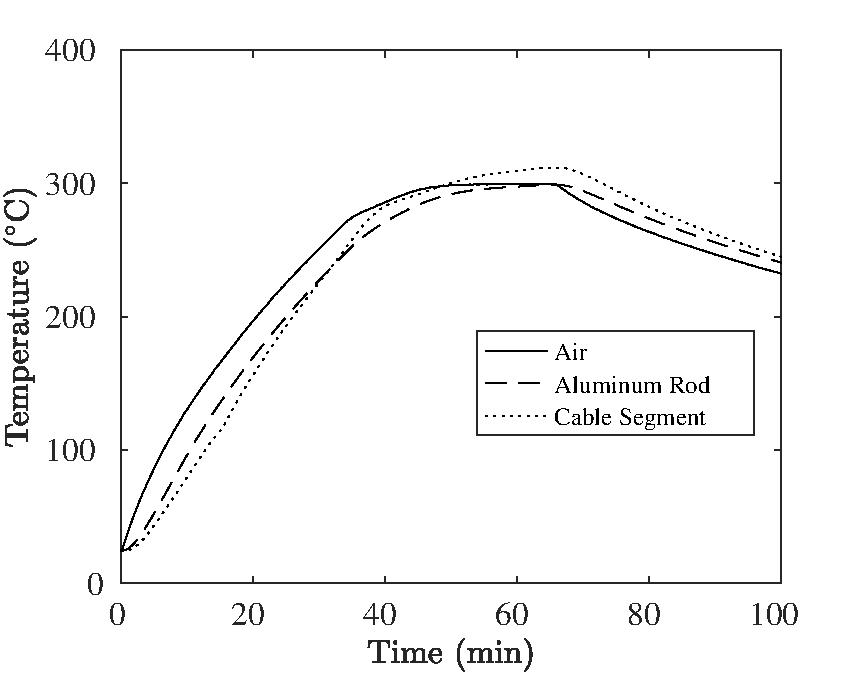
\includegraphics[height=3.0in]{../SCRIPT_FIGURES/Oven_Test}
\caption[Temperatures of cables and aluminum rod in convective oven]{Measured temperatures of a 13~mm (0.5 in) aluminum rod and two representative cable segments in a convection oven.}
\label{oven}
\end{figure}

The measured temperatures of the rod and cable segments are fairly comparable, suggesting that the aluminum rod mimics the cable segments until the cable polymers begin to pyrolyze at approximately 300~$^\circ$C. However, in the experiments described below, the temperature of the aluminum rod tended to increase at a slightly faster rate than instrumented cables located at the same location. There are several reasons for this. First, the cables were cut into lengths on the order of 3~m to 4~m (9~ft to 12~ft) and placed in a ladder-back cable tray. Only a small fraction of the cable was exposed to the direct heat of the fire plume, and its copper conductors would have distributed the heat along its entire length. The aluminum rod, on the other hand, is cut to a length of 15~cm; thus, the heat is ``trapped'' and does not dissipate laterally. Second, the cables were set next to one another in the tray such that some fraction of the surface area would have been shielded from the convective and radiative heating of the fire. The rods were typically more exposed.

Given that the aluminum rods are not perfect surrogates for cables, why use them at all? It is not difficult to affix thermocouples within unenergized cables, and, indeed, this was done as part of the test protocol. The principal reason for the aluminum rods is to facilitate comparisons with numerical models. Regardless of the level of detail in the underlying physics, fire models typically treat a cable as a cylinder that is heated uniformly at the surface and which undergoes one-dimensional heating in the radial direction. There is no lateral heat conduction and typically there are no nearby obstructions. It is certainly possible to model a tray full of cables using a complex three-dimensional heat conduction algorithm, but such a calculation is time-consuming, difficult to embed within existing models, and requires detailed thermo-physical data of all the cables that might be in a given tray. It is far more tractable to perform a simple one-dimensional heat transfer calculation based on computed conditions in the vicinity of the cable tray. The computed surrogate temperatures can also be easily scaled should the actual cables be larger or smaller in diameter to the nominal 13~mm (0.5~in) chosen in this study.

The temperature measurements described in this report are to be used to validate numerical models that will then be used to consider many other enclosure-cable tray configurations that could not be physically tested. The purpose of this modeling is to predict the thermal conditions in the vicinity of equipment surrounding a burning electrical enclosure. The aluminum rods provide a far better ``target'' with which to assess the model predictions. In essence, the aluminum rod is a device that measures the amount of heat that would be absorbed by an actual cable of comparable diameter. Making this measurement with the cable itself is, ironically, more difficult because of the fact that the cable allows the absorbed heat to be conducted along its length.

\newpage

\section{Circuit Breaker Heat Release Rate Measurements}
\label{Sec:Circuit Breakers}

Four low-voltage circuit breaker enclosures built by ABB, an international manufacturer of electrical equipment, were shipped to the National Fire Research Laboratory (NFRL) at NIST in September 2023. These enclosures were donated by the German nuclear safety organization Gesellschaft für Anlagen- und Reaktorsicherheit (GRS) from a decommissioned nuclear power plant in Germany, and contain low-voltage circuit breakers and various types of panel wires, cables, and instrumentation. One configuration consisted of three vertical sections that were bolted together, as shown in Fig.~\ref{fig:Cabinet_1}, and one configuration was detached.

\begin{figure}[ht]
\centering
\includegraphics[width=\textwidth]{../FIGURES/Large_Cabinet}
\caption[Photograph of ABB enclosure] {Photograph of the ABB enclosure. The breaker is located in the middle compartment of each vertical column. Wiring and other electrical equipment is located mainly in the compartment above, and the compartment below is largely empty. Each of the three vertical columns is largely the same.}
\label{fig:Cabinet_1}
\end{figure}

Two additional circuit breaker enclosures, manufactured by Westinghouse, were shipped to NIST in December 2023. Each enclosure houses six low-voltage breakers. One of the enclosures is shown in Fig.~\ref{fig:Cabinet_2}, where the lowest level breaker has been removed and replaced with a gas burner for the experiment. The uppermost compartment contains wiring and instrumentation.

\begin{figure}[ht]
\centering
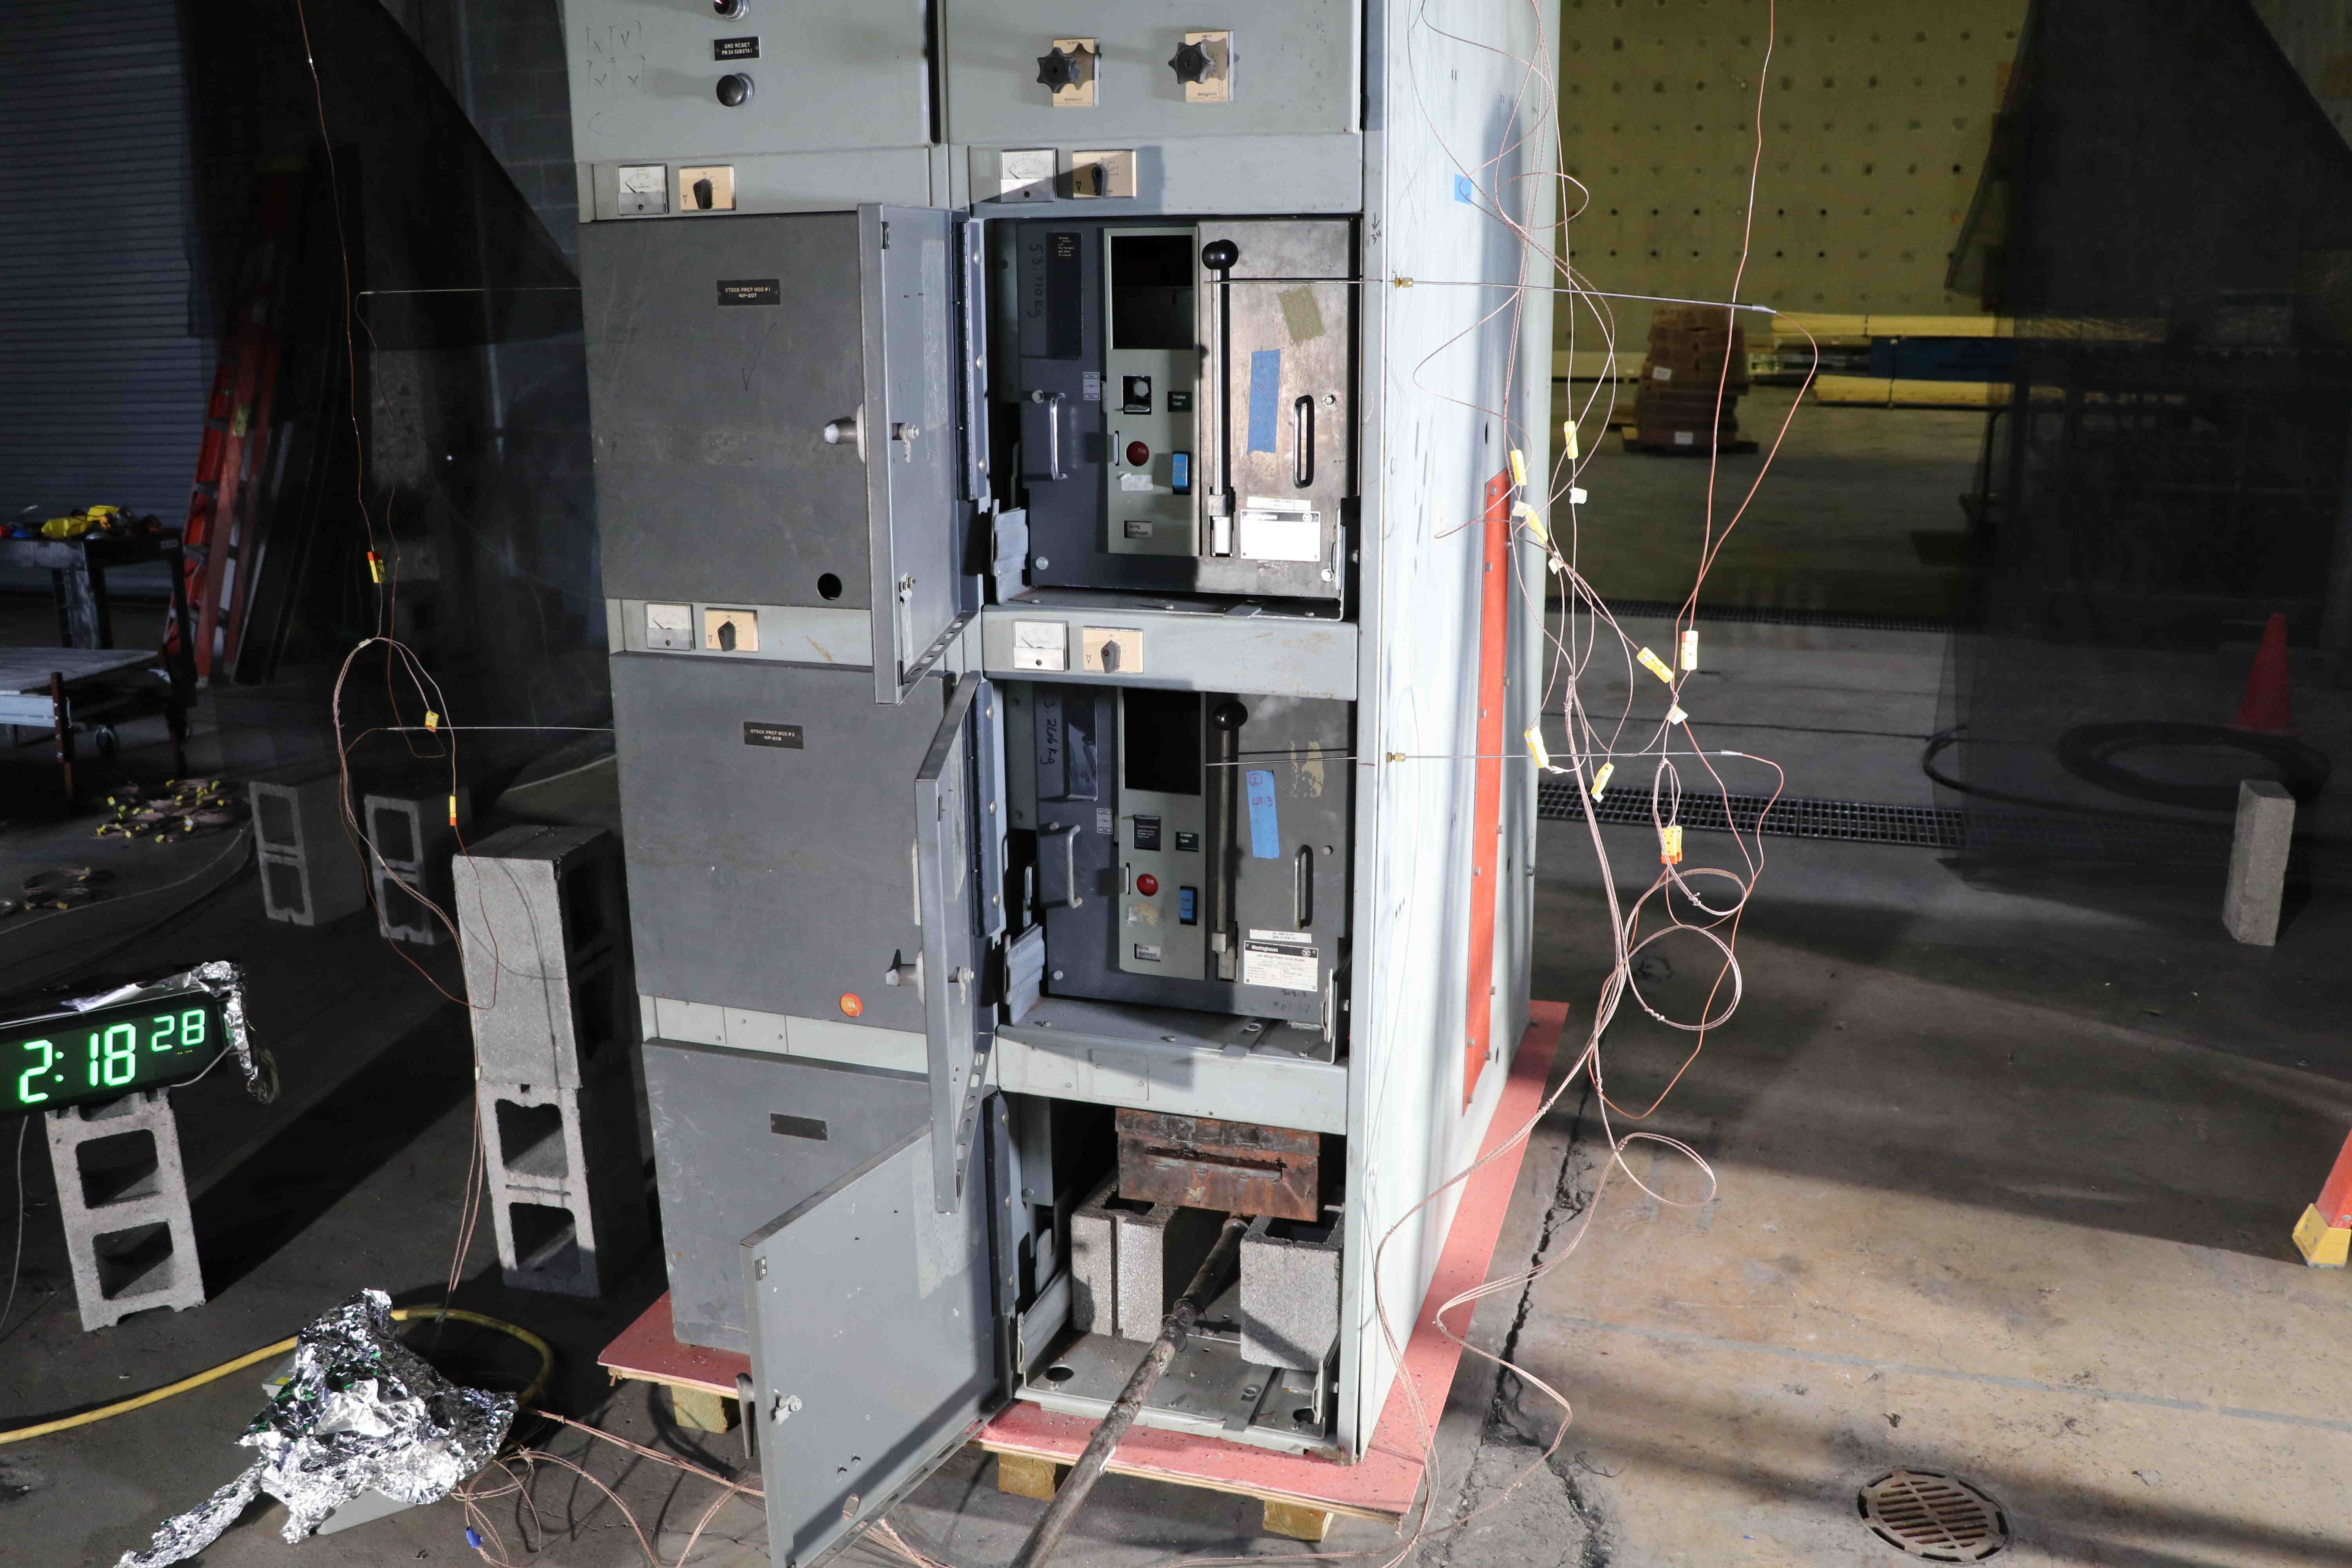
\includegraphics[width=\textwidth]{../FIGURES/Westinghouse}
\caption[Photograph of Westinghouse enclosure] {Photograph of the Westinghouse enclosure. Each vertical column contains three breakers in the lowest three compartments, with instrumentation in the uppermost compartment. A gas burner has replaced the lowest level breaker in the right vertical column.}
\label{fig:Cabinet_2}
\end{figure}

\subsection{Description of Experiments}

For the experiments involving either the ABB or Westinghouse enclosures, one or more circuit breakers with nominal dimensions of 30~cm by 40~cm by 30~cm (12~in by 16~in by 12~in) and masses of approximately 50~kg (110~lb) are the primary combustibles whose non-metallic mass consists of polymeric insulating materials such as glass-polyester and thermoset composite resins. Additionally, plastic wire harnesses, panel wire, and circuit boards are located, typically, in the compartment above the breaker, as seen in Fig.~\ref{fig:Contents}. There are, typically, only a few jacketed, multi-conductor cables located within the upper compartment. In these experiments, some cables were added to the upper compartment to make up for those that were removed prior to shipment to NIST.

The compartment below the breaker is largely devoid of combustible materials. No attempt was made to remove and weigh all of the combustible materials because doing so would have potentially changed its burning behavior. However, representative samples of the most common non-metallic components such as wire insulation, switches, and circuit boards were removed prior to the experiments to determine their heat of combustion (see Section~\ref{ssec:MCC}). Estimates of the total combustible mass in each compartment were then made by dividing the integral of the HRR with time (kJ) by the measured heat of combustion (kJ/kg). These results are presented in Section~\ref{sec:results}.

\begin{figure}[t]
\centering
\includegraphics[width=\textwidth]{../FIGURES/Contents}
\caption[Photograph of instrumentation above the breaker] {Photograph of instrumentation above the breaker. A few cables have been added to replace those removed previously.}
\label{fig:Contents}
\end{figure}

The breakers were ignited using a nominally 30~cm (12~in) square natural gas burner positioned approximately 20~cm (8~in) beneath the circuit breaker, as shown in Figs.~\ref{fig:Cabinet_2} and~\ref{fig:Burner}. The burner's HRR\footnote{The relative expanded uncertainty (95~\% confidence interval) of the HRR measurement under the hood used in these experiments is 4~\% for natural gas and 7~\% for ``generic combustibles''~\cite{bryant2019nist}.} was set to approximately 100~kW. After sustained ignition of the circuit breaker was observed, the burner was turned off and the enclosure fire was allowed to continue burning until the measured HRR decreased below 10~kW, at which point the small remaining fires were extinguished.

\begin{figure}[ht]
\centering
\includegraphics[width=\textwidth]{../FIGURES/Burner}
\caption[Position of the burner] {Position of the burner under the breaker in Test~34.}
\label{fig:Burner}
\end{figure}

Sheathed thermocouples\footnote{Type K, sheath diameter 3~mm (1/8~in), expanded uncertainty $\pm 0.75$~\% of the measured absolute temperature.} were installed approximately 15~cm (6~in) below the ceiling of each compartment to provide a measurement of the gas temperature within. Thermocouples were also embedded within electrical cable segments and aluminum rods (see Section~\ref{cable_surrogate}) that were placed directly above each circuit breaker. The cable target is a 7-conductor thermoplastic electrical cable segment and the aluminum target is a 6061~aluminum alloy rod, both approximately  15~cm (6~in) in length and 13~mm (0.5~in) in diameter. Throughout this report, these surrogate targets are referred to as slug calorimeters, or simply ``slugs,'' a term commonly used in the fire science community to describe objects such as these.

Photographs of the enclosures used in this project are shown in Figs.~\ref{fig:Cabinet_1} and \ref{fig:Cabinet_2}. Each enclosure is approximately 2.2~m (87~in) tall, 0.4~m (16~in) wide, and 1.0~m (40~in) deep. Some of the enclosures have ventilation panels near the top and bottom, and all have seams and small openings to accommodate wiring, bus bars, door panels, and so on. No attempt was made to seal these various gaps and openings except in Experiment~34 where a burned out instrument panel was covered by a steel plate, and in Experiment~35, where a hole in the top of the enclosure was covered by a steel plate.



\subsection{Experimental Results}
\label{sec:results}

The measurements of the HRR of the breakers were made in October of 2023 and January of 2024. Nominal results are listed in Table~\ref{matrix} and details can be found on the following pages. For each experiment, the nominally 100~kW natural gas burner was sustained until it appeared that the breaker had begun to burn. For the first two experiments, the burner was sustained longer than necessary, as evidenced by Exp.~35 where the breaker was able to sustain a fire after four minutes of exposure from the burner.

Overall, the breakers within the ABB enclosures sustained a fire beyond the time when the burner was extinguished. However, the Westinghouse breakers did not appear to burn without the aid of the gas burner, even though, after the experiment, the non-metallic materials within the breaker clearly showed evidence of having pyrolized. In short, the pyrolysis was not followed by flaming combustion.

The ``Peak HRR'' in Table~\ref{matrix} indicates the maximum value of the HRR of the enclosure contents; that is the total HRR minus that of the natural gas burner. The ``Total HR'' (Total Heat Release) is the total energy released less the burner's energy; that is, the energy of the contents alone. The ``Mass Consumed'' is the Total HR divided by an estimated\footnote{The uncertainty of the estimated heat of combustion is difficult to quantify. The estimated value of 20~MJ/kg $\pm$5~MJ/kg is merely the average heat of combustion, $\Delta H_c$, measured for various plastics found within the enclosure (weighted to account for the greater mass of combustible solids contained within the circuit breaker itself, which had relatively low $\Delta H_c$; see Sec.~\ref{ssec:MCC}).} heat of combustion of 20~MJ/kg for the combustible materials within the enclosure. The peak ``slug'' and gas temperatures are comparable and represent uniform conditions within the burning breaker and instrument compartments.


\begin{table}[ht]
\begin{center}
\caption[Summary of Experimental Results]{Summary of Experimental Results. The uncertainty of the HRR is $\pm 7$~\%. The uncertainty of the temperature is $\pm 0.75$~\% of its absolute value. The listed times are rounded to the nearest minute.}
\label{matrix}
\begin{tabular}{|c|c|c|c|c|c|c|c|c|}
\hline
Exp.   &                & Peak          & Total   & Mass            & Time            & Burner       & Peak Slug    & Peak Gas      \\
No.    & Make           & HRR           & HR      & Consumed        & to Peak         & Duration     & Temp.        & Temp.         \\
       &                & [kW]          & [MJ]    & [kg]            & [min]           & [min]        & [$^\circ$C]  & [$^\circ$C]   \\ \hline
33     & ABB            & 250           & 387     & 19.4$\pm$4.9    & 11              & 10           & 770          & 860           \\ \hline
34     & ABB            & 140           & 192     & 9.6$\pm$2.4     & 9               & 8            & 680          & 700           \\ \hline
35     & ABB            & 200           & 230     & 11.5$\pm$2.9    & 20              & 4            & 680          & 670           \\ \hline
40     & West.          & 30            & 60      & 3.0$\pm$0.8     & 28              & 60           & 160          & 650           \\ \hline
41     & West.          & 100           & 280     & 14.0$\pm$3.5    & 40              & 60           & 150          & 700           \\ \hline
\end{tabular}
\end{center}
\end{table}

The breaker that was burned in Exp.~35 was weighed before and after the experiment. Its original mass was 47.8~kg and its final mass was 44.1~kg. The uncertainty of the load cell is approximately 1~g, which is far exceeded by the uncertainty due to extracting the burned breaker from the enclosure and separating out materials that were or were not part of the original breaker. Thus, the estimated combustible mass of the breaker is taken as 3.7~kg~$\pm$~0.1~kg.

Using the measured mass loss of the breaker and the estimates of the mass consumed in the three experiments, it is possible to estimate the distribution of combustible mass in the lower, middle, and upper compartments of the enclosure. In Exp.~33, the fire consumed the contents of a lower, middle and three upper compartments. In Exp.~34, the fire consumed a lower and middle compartment. In Exp.~35, the fire consumed a lower, middle, and upper compartment. Taking the combustible load of the middle compartment to be 3.7~kg, the estimated mass loss of the breaker, a least squares regression yields an estimate of 3.5~kg for the lower compartment and 2.7~kg for the upper. The 3.5~kg estimate for the lower compartment can be taken as all of the combustibles in the lower and middle compartment minus the breaker itself. These estimated combustible loads fall well within the uncertainty bounds for the total mass consumption listed in Table~\ref{matrix}.

The HRR of a fire contained within a single compartment is limited by the air supplied through openings in the back and side of the enclosure and the opening in the front door of the compartment that is created when the instrument panel melts/burns away. For the enclosures tested, this opening is approximately 15~cm (6~in) wide by 30~cm (12~in) tall. A useful correlation~\cite{SFPE:Walton} used in compartment fire modeling states that air is entrained into a flashed over compartment at a rate given by
\begin{equation}
   \dot{m}_{\rm a} = 0.5  \, A \, \sqrt{H}  \approx 0.0123 \; \hbox{kg/s}
\end{equation}
where $H$ is the opening height (0.3~m) and $A$ is the opening area (0.045~m$^2$). With this estimate, the HRR can be estimated
\begin{equation}
   \dot{Q} = Y_{\rm O_2,\infty} \, E \, \dot{m}_{\rm a} \approx 37 \; \hbox{kW}
\end{equation}
where $Y_{\rm O_2,\infty}\approx 0.23$ is the oxygen mass fraction of air and $E\approx 13\,100$~kJ/kg is the approximate amount of energy released per unit mass of oxygen consumed.

Evidence for the estimated HRR associated with the opening of the instrument panel can be seen in Exp.~35 where the upper compartment opens up at approximately 19~min, at which time the HRR increases rapidly by approximately 40~kW. The increased ventilation through the front door adds to the existing ventilation through the back of the enclosure. Collectively, these openings supply the air needed to support an HRR of approximately 100~kW per compartment.


\subsubsection{Material Property Measurements}
\label{ssec:MCC}

Material samples were taken from the various circuit breakers to better understand their burning behavior using a Microscale Combustion Calorimeter\footnote{This MCC used in this work was a Deatak MCC-3 equipped with a paramagnetic oxygen sensor and calibrated according to ASTM~D7309~\cite{ASTMD7309}} (MCC), an apparatus in which a specimen of known mass is thermally decomposed in nitrogen at a constant heating rate and then burned in oxygen to determine its heat of combustion. Samples were not identified by a specific material type (e.g., composition, and/or manufacturer/distributor name), rather they are labeled in series (No. 1 to No. 10) to correspond to each of the items identified in Fig.~\ref{fig:MCC_samples}.


\begin{figure}[!ht]
\begin{tabular*}{\textwidth}{l@{\extracolsep{\fill}}r}
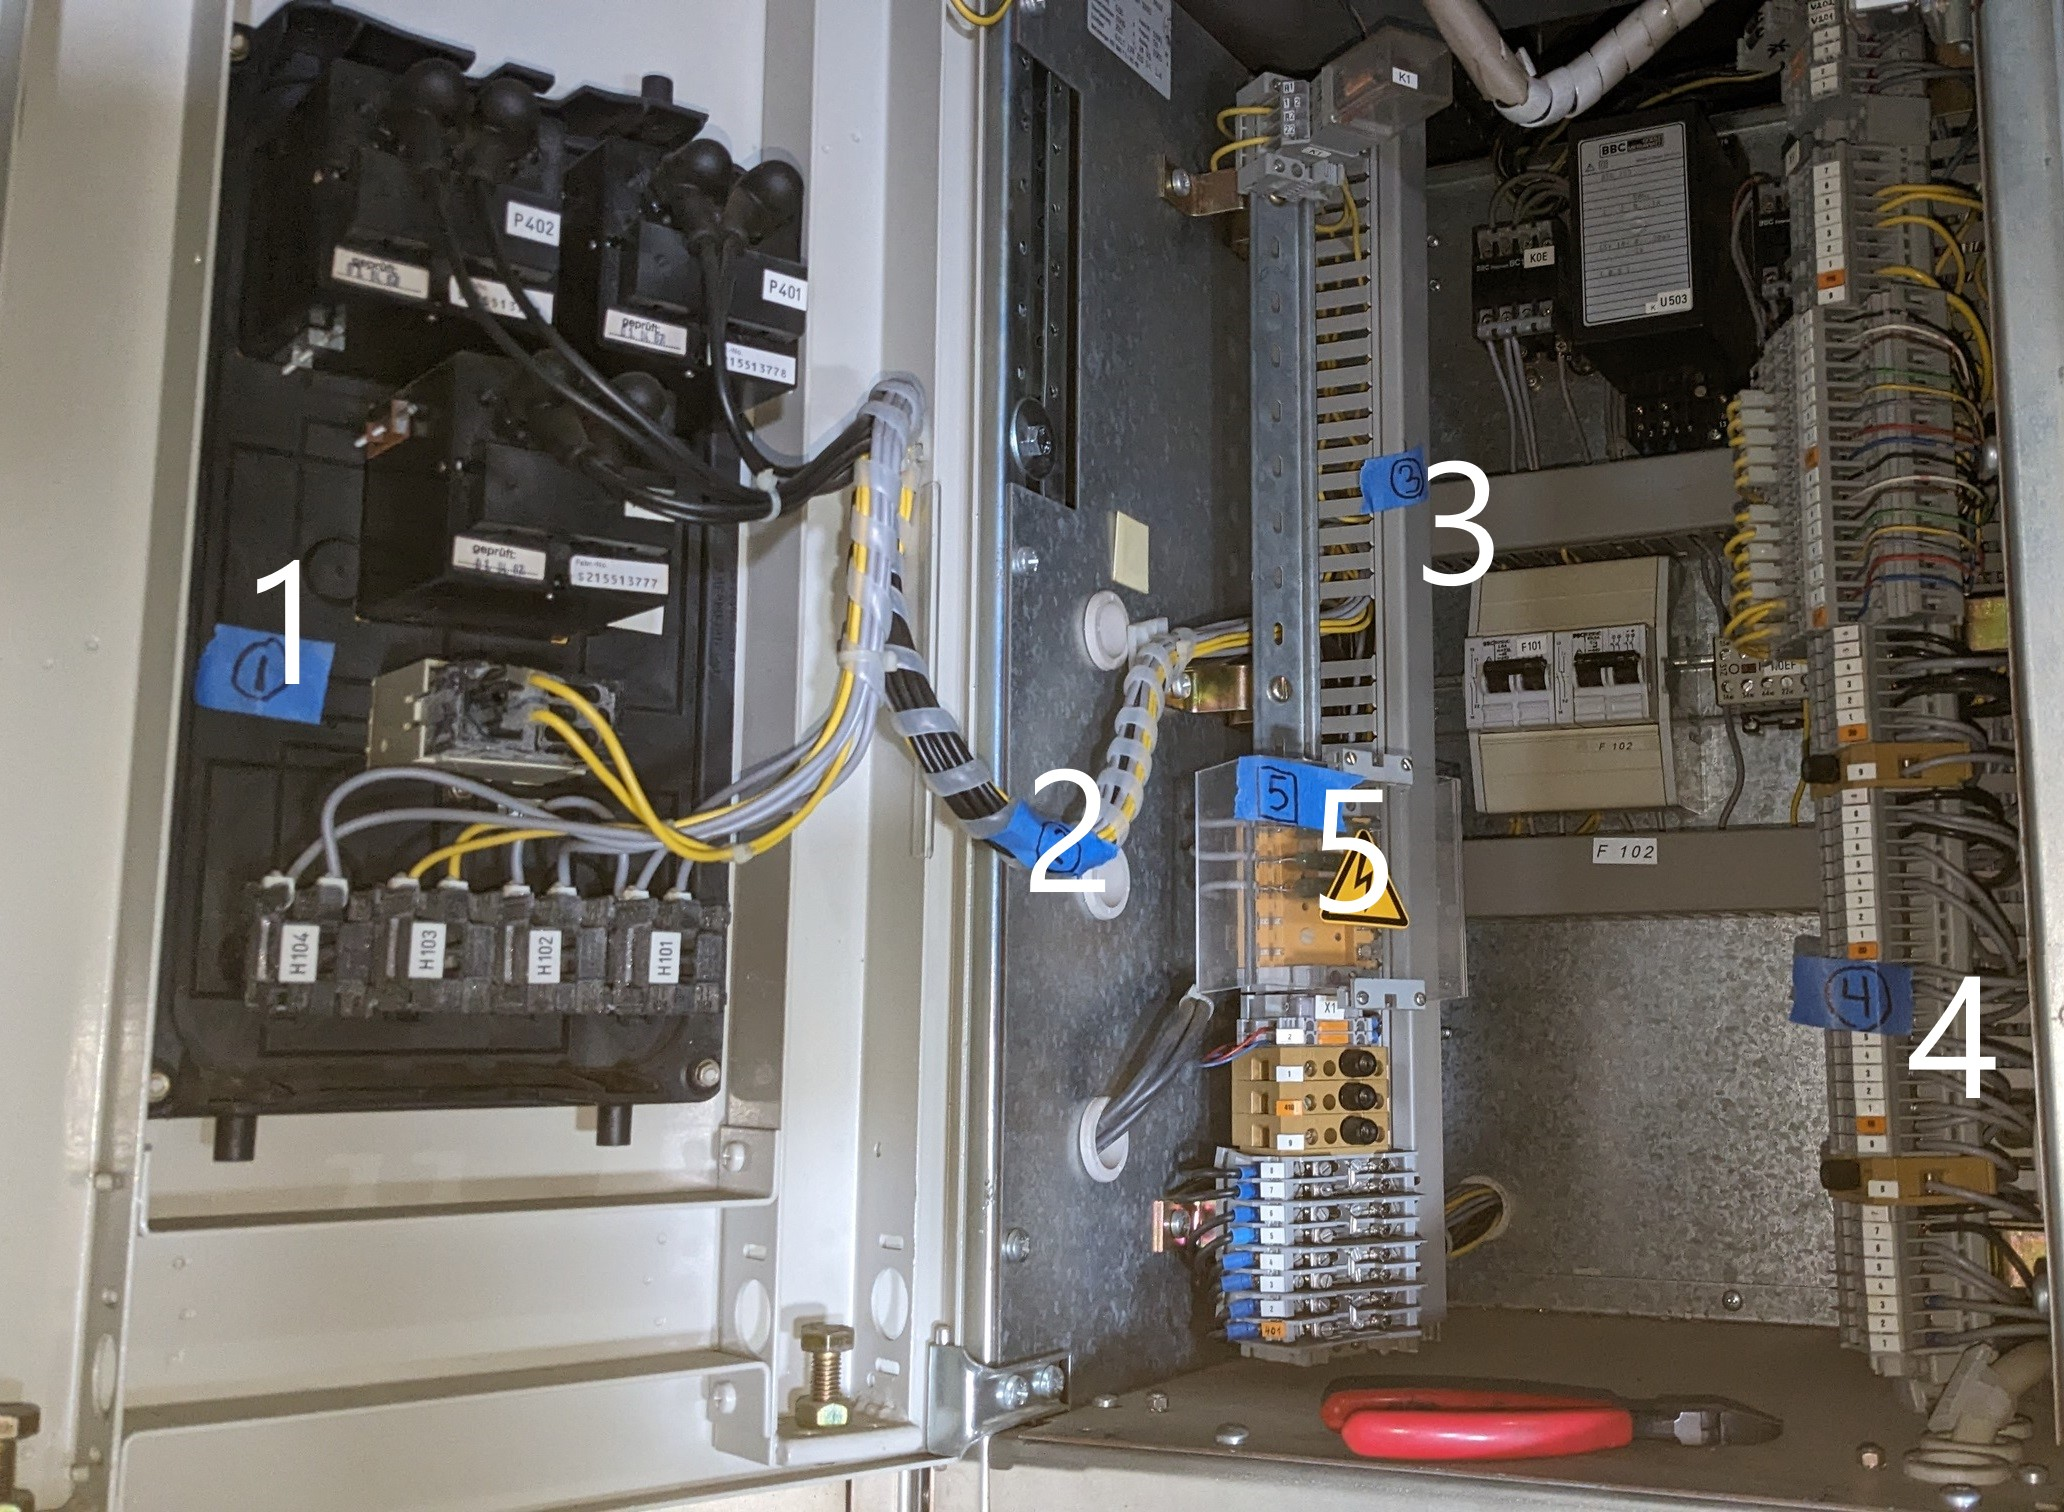
\includegraphics[height=2.40in]{../FIGURES/Cabinet_Materials1.jpg} &
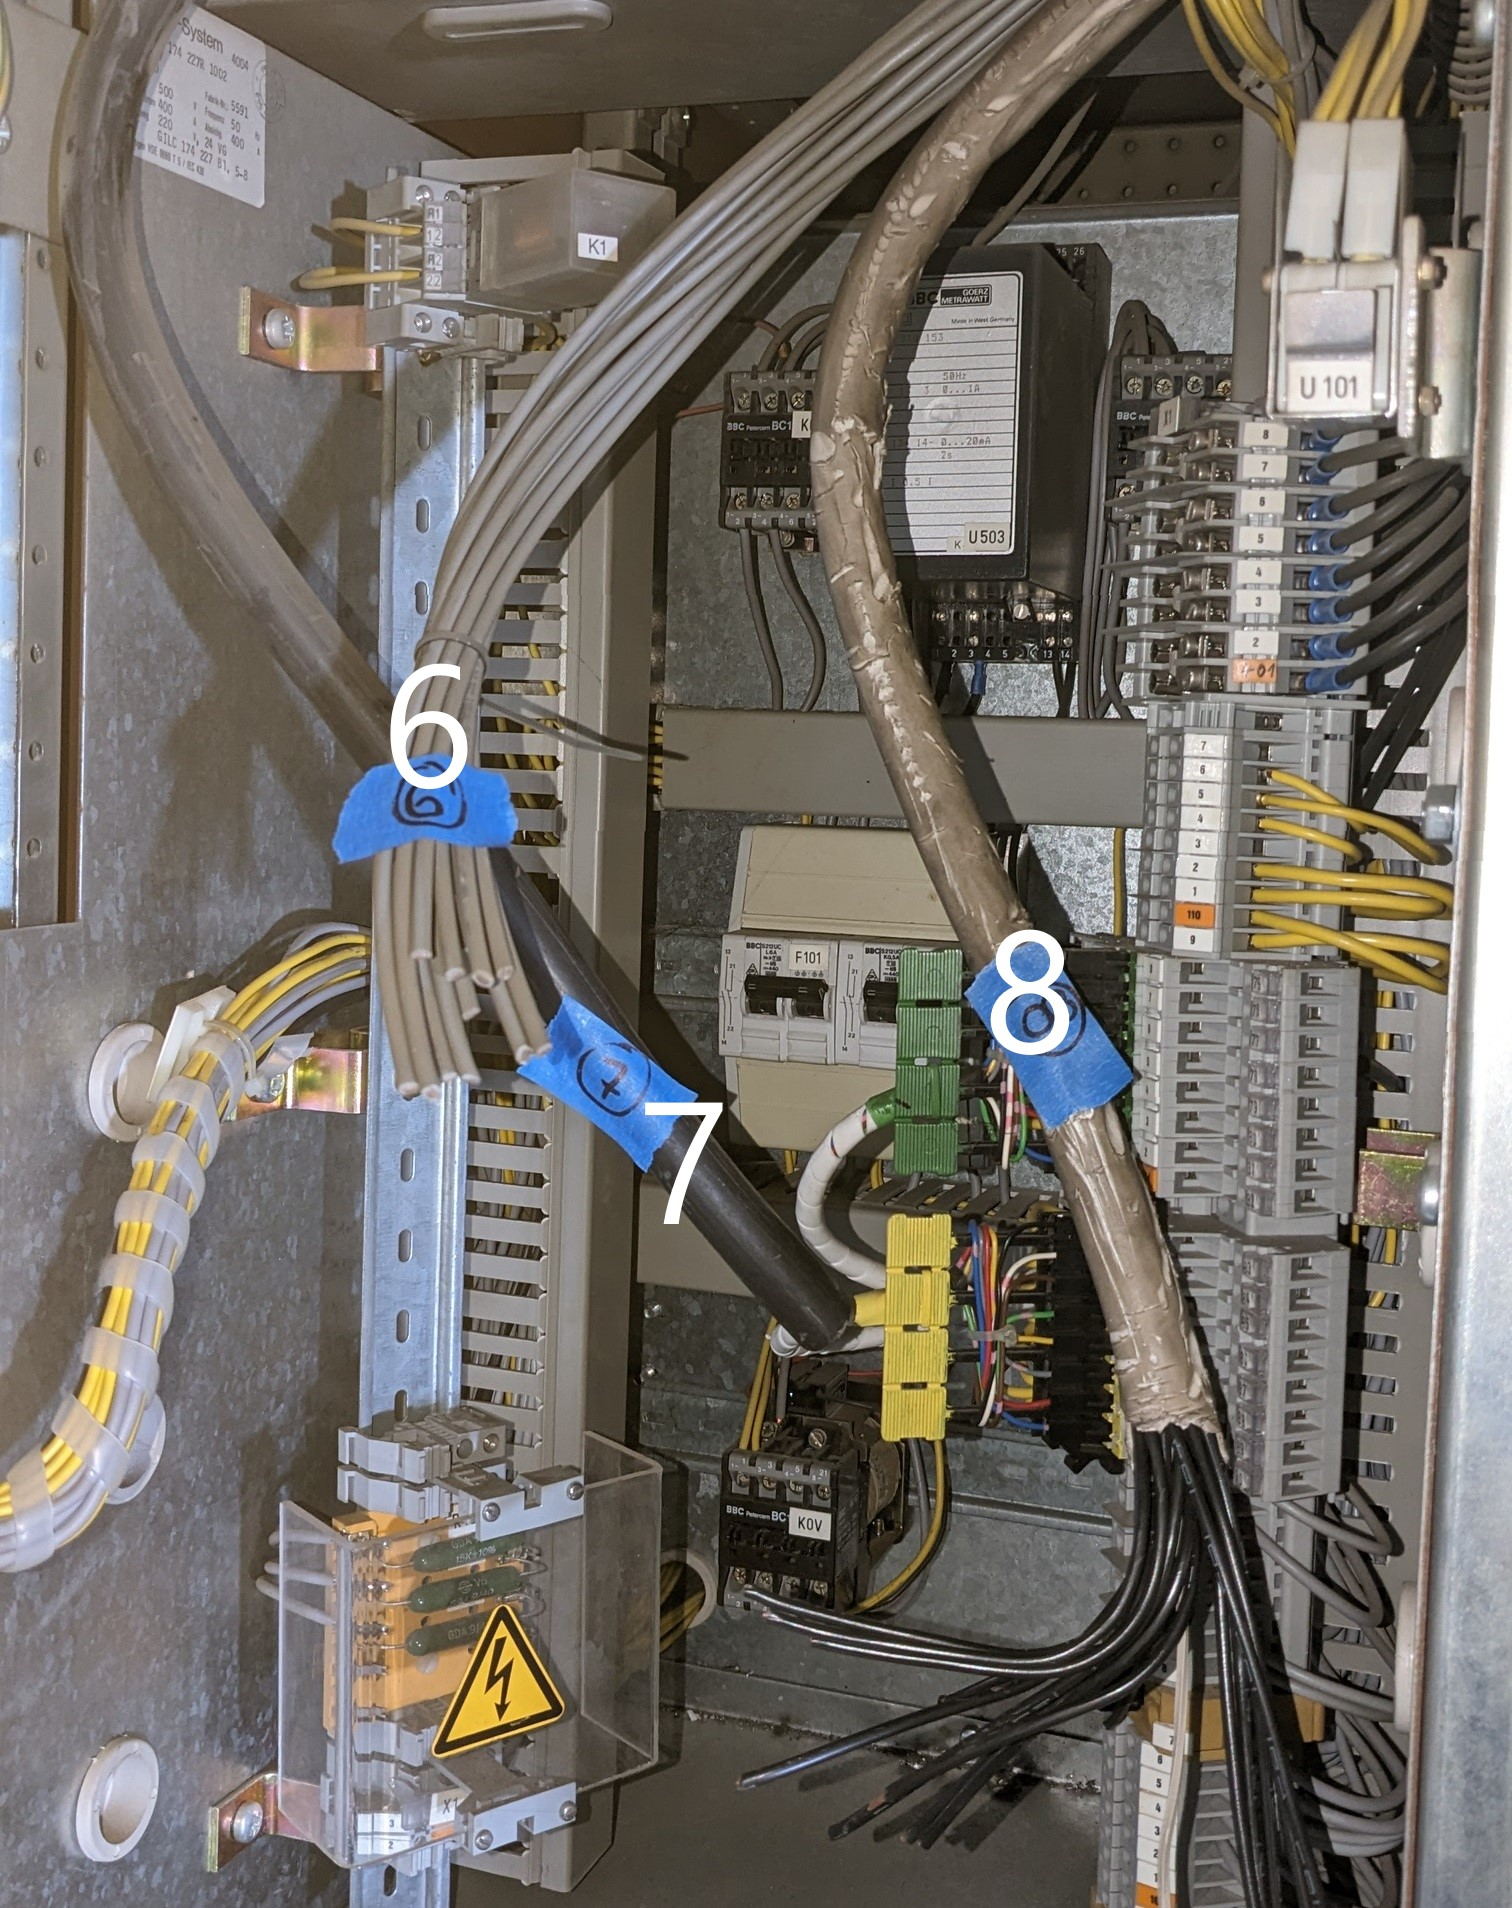
\includegraphics[height=2.40in]{../FIGURES/Cabinet_Materials2.jpg} \\
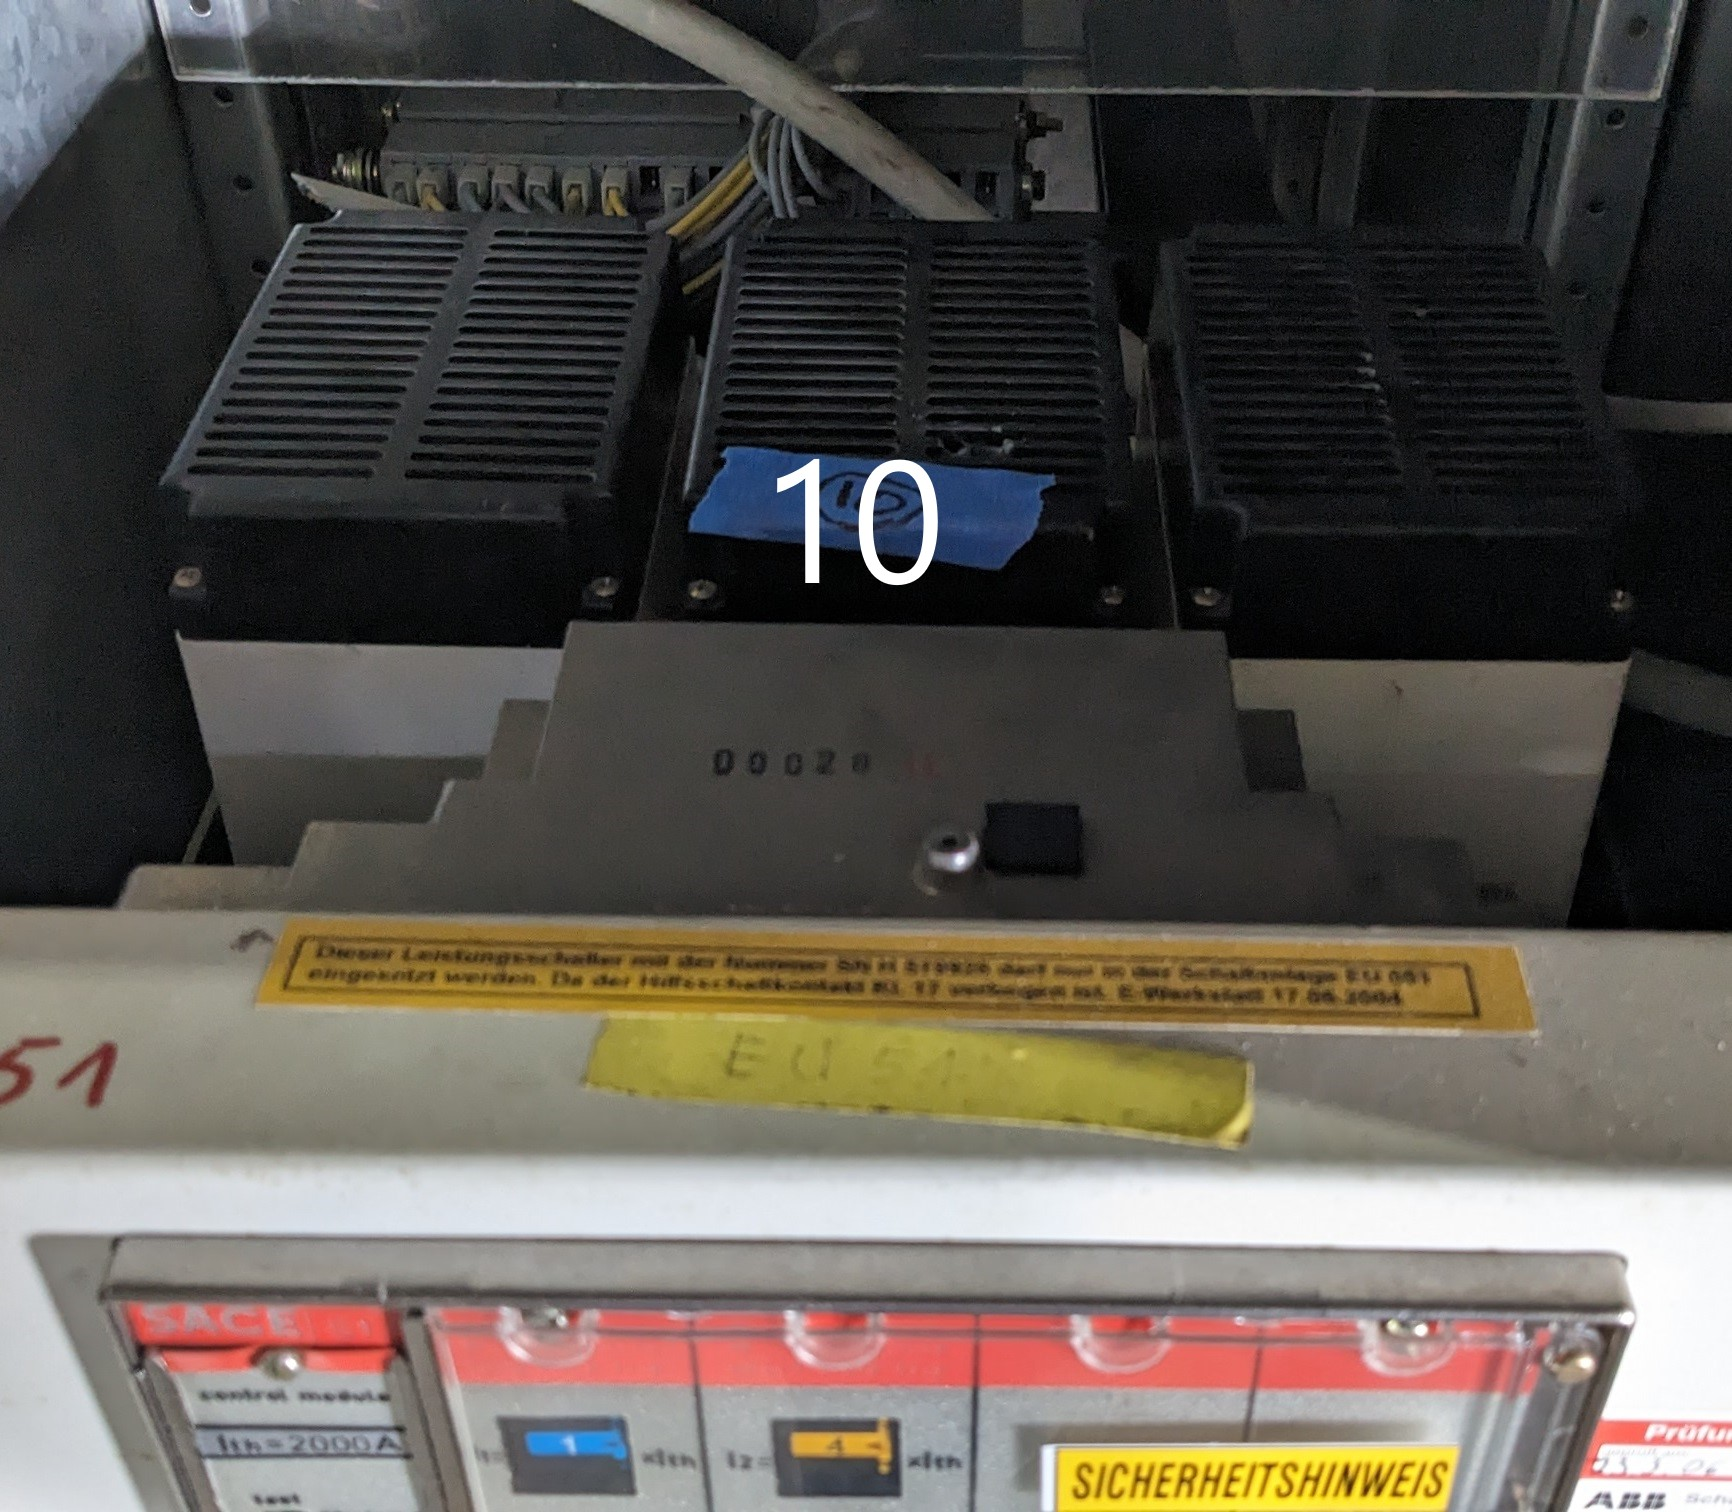
\includegraphics[height=2.40in]{../FIGURES/Cabinet_Materials4.jpg} &
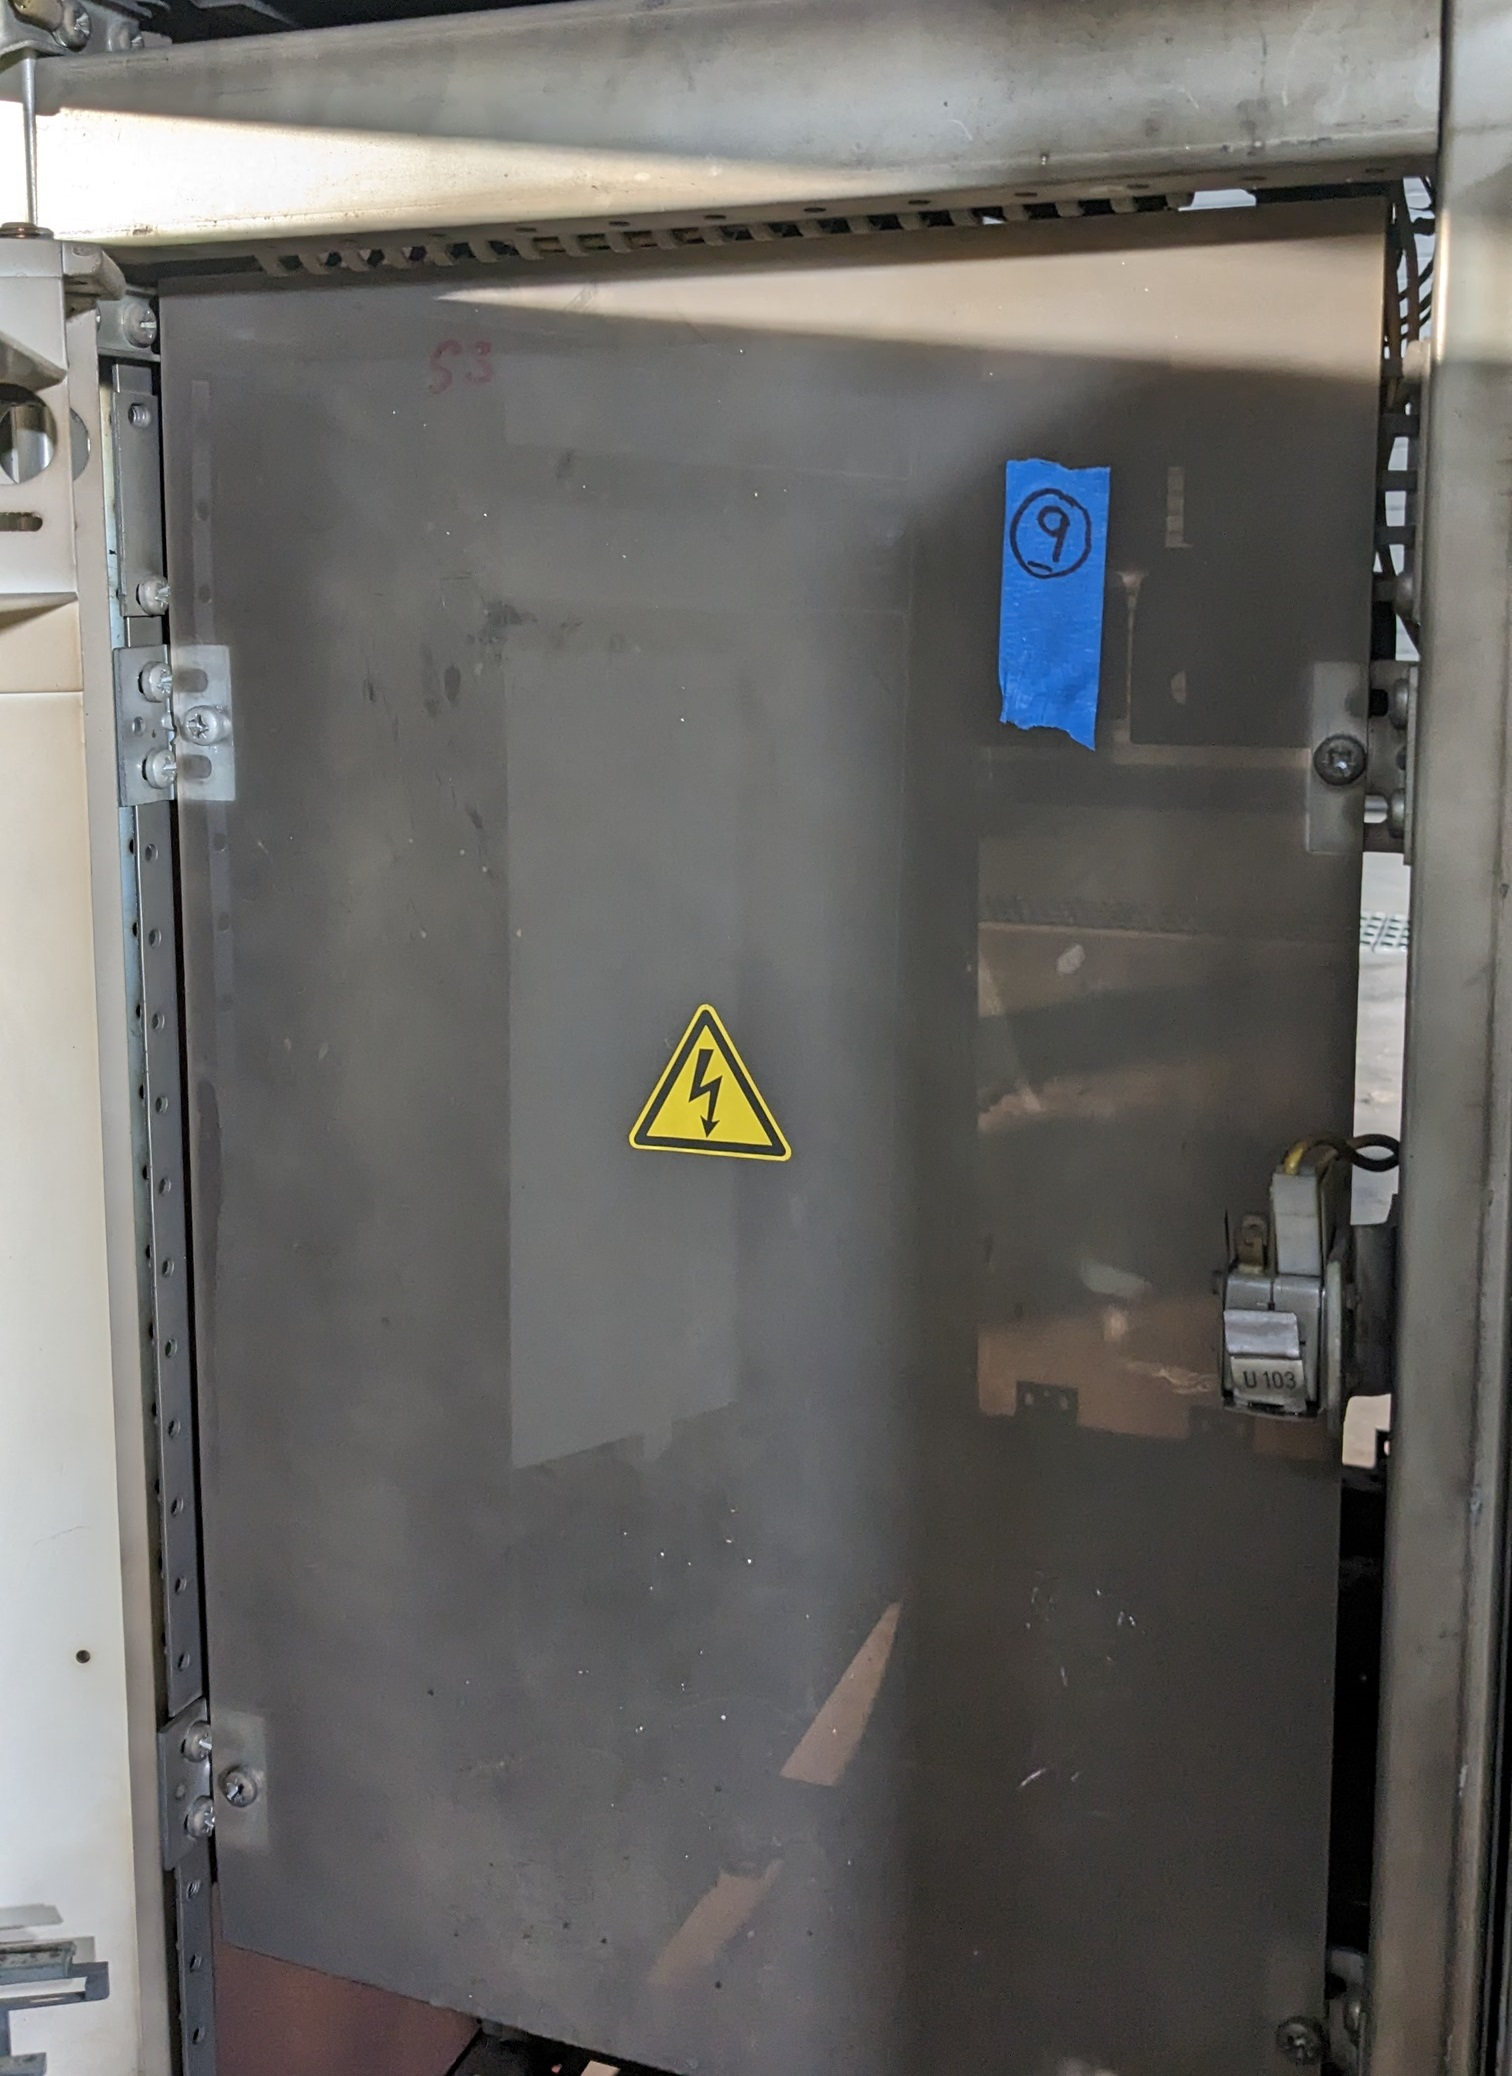
\includegraphics[height=2.40in]{../FIGURES/Cabinet_Materials3.jpg}
\end{tabular*}
\caption[Electrical components selected for MCC measurements] {Photographs of each of the ten components selected for MCC measurements.}
\label{fig:MCC_samples}
\end{figure}

MCC experiments were conducted in December, 2023. The material samples were subjected to a 80~mL/min nitrogen stream starting at a temperature of 75~°C, increasing linearly to 750~°C at a heating rate of 60~K/min. The pyrolyzed gases were combusted in an oxygen stream of 20~mL/min. Tests were repeated at least three times for each material. Nominal results are listed in Table~\ref{MCC}. The mass-weighted average heat of combustion of the materials tested is approximately 20~MJ/kg. Also reported in this table are the onset temperature and Fire Growth Capacity, FGC. The FGC is a physically-based parameter for early stage fire growth, derived from a simple burning model, that has been shown to rank commercial materials according to their behavior in bench scale flame and fire tests~\cite{lyon2021molecular}. The onset temperature is approximated by the temperature at which 5~\% of total heat release is measured, consistent with the definition of the FGC. Details of these calculations are provided elsewhere~\cite{DOT/FAA/TC-20/30, lyon2021molecular}.


\begin{table}
\caption[MCC Measurements]{MCC Measurements. The relative expanded uncertainty in the reported Heat of Combustion is approximately 6~\% of the measured value. The primary components of this uncertainty estimate include: (1) the relative expanded uncertainty of the heat released per unit mass of oxygen consumed, 5~\%~\cite{Huggett:1}; (2) the relative expanded uncertainty of the system flow rate, 2~\%; and (3) test repeatability, 2~\% or 2 standard deviations of replicate measurements. The relative expanded uncertainty in the solid residue yield is 2~\%, primarily due to stochastic variations in values measured in repeated tests. The expanded uncertainty of the temperature measurements is $\pm 0.75$~\% of the measured absolute value. }
\label{MCC}
\begin{minipage}{\textwidth}
\begin{tabular}{ccccc}
\hline
Matl.  & Heat of        & Solid Residue    & Onset              & Fire Growth             \\
No.    & Combustion     & Yield            & Temperature        & Capacity (FGC)          \\
       & (kJ/g)         & (g/g)            & (°C)               & (J/(g~K))               \\ \hline
3      &  13.9          & 0.29             & 315\footnote{Material 3 decomposes through a multi-step reaction, approximately 10\% of total heat release occurs in reaction step 1; onset temperature of second main reaction step is approximately 425~$^\circ$C.}     & 80             \\
4      &  30.8          & 0.02             & 388                & 376                     \\
5      &  25.7          & 0.00             & 354                & 465         \\
6      &  28.3          & 0.10             &                    &              \\
7      &  22.1          & 0.40             & 248                & 111            \\
8      &   9.6          & 0.02             & 257                &  78           \\
9      &  27.1          & 0.24             & 507                & 310             \\
10     &  17.9          & 0.57             & 204                &  67            \\
\hline
\end{tabular}
\end{minipage}
\end{table}



\clearpage

\subsubsection{Experiment 33}

The HRR and gas/target temperatures are shown in Fig.~\ref{fig:Test_33}. Referring to the photographs shown in Fig.~\ref{fig:Test_33_photos}, the natural gas burner was positioned near the top of the lower left compartment of the enclosure, approximately 20~cm (8~in) below the breaker located in the middle left compartment. The fire ignited the breaker after approximately 2~min and then spread to the compartment above. The fire then spread to the two adjacent compartments along the top of the enclosure. The gas temperatures shown in Fig.~\ref{fig:Test_33} indicate that the fire spread from one compartment to the next in approximately 10~min. The compartments are separated by two steel walls.

\begin{figure}[!ht]
\begin{tabular*}{\textwidth}{l@{\extracolsep{\fill}}r}
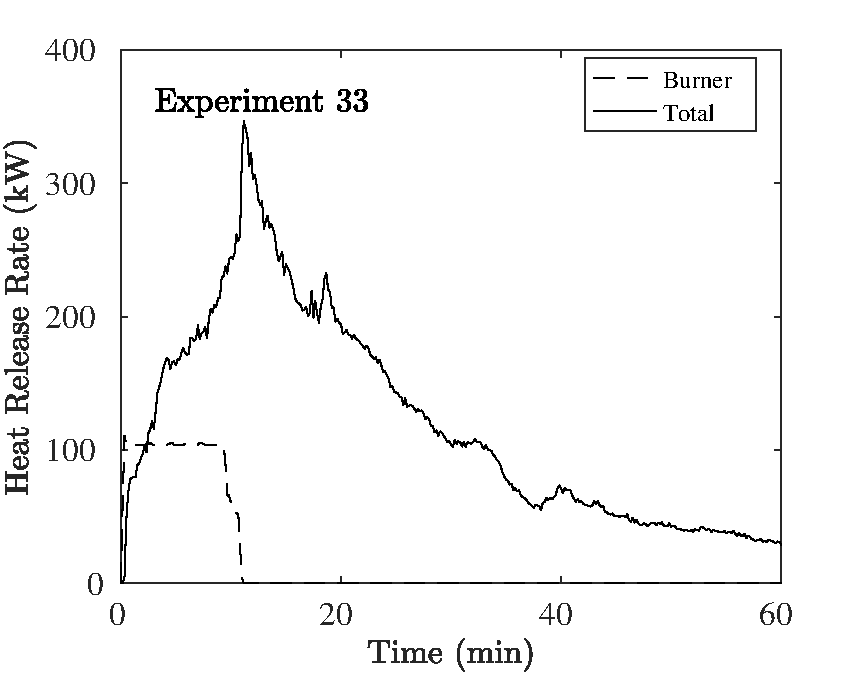
\includegraphics[height=2.2in]{../SCRIPT_FIGURES/Test_33_HRR} &
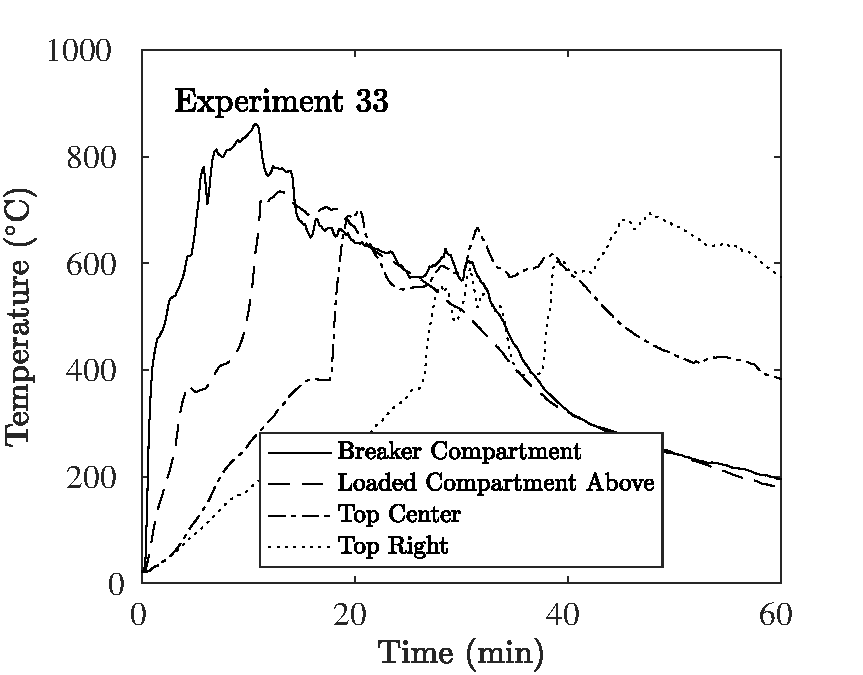
\includegraphics[height=2.2in]{../SCRIPT_FIGURES/Test_33_Gas_TC} \\
\multicolumn{2}{c}{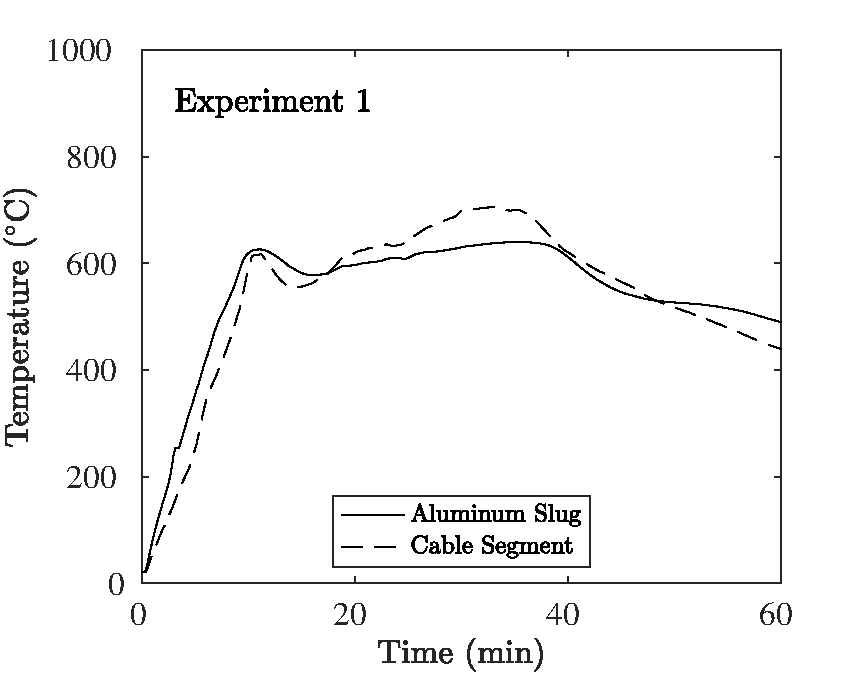
\includegraphics[height=2.2in]{../SCRIPT_FIGURES/Test_33_Slug_TC}}
\end{tabular*}
\caption[HRR and temperatures of Exp.~33]{Heat release rate (upper left), gas temperatures (upper right), and slug/cable temperatures (bottom) for Exp.~33. The curve labeled ``Burner'' in the upper left plot represents the ideal HRR based on natural gas flow, and ``Total'' is the HRR measured via oxygen-consumption calorimetry. The gas temperatures were recorded near the ceiling of the middle left compartment housing the breaker (``Breaker Compartment''), the upper left compartment housing miscellaneous wiring and plastics (''Loaded Compartment Above''), and the upper central and upper right compartments housing similar materials (``Top Center'' and ``Top Right''). In the bottom plot, the ``Aluminum Slug'' and thermoplastic ``Cable Segment'' were placed atop the breaker.}
\label{fig:Test_33}
\end{figure}

\begin{figure}[p]
\centering
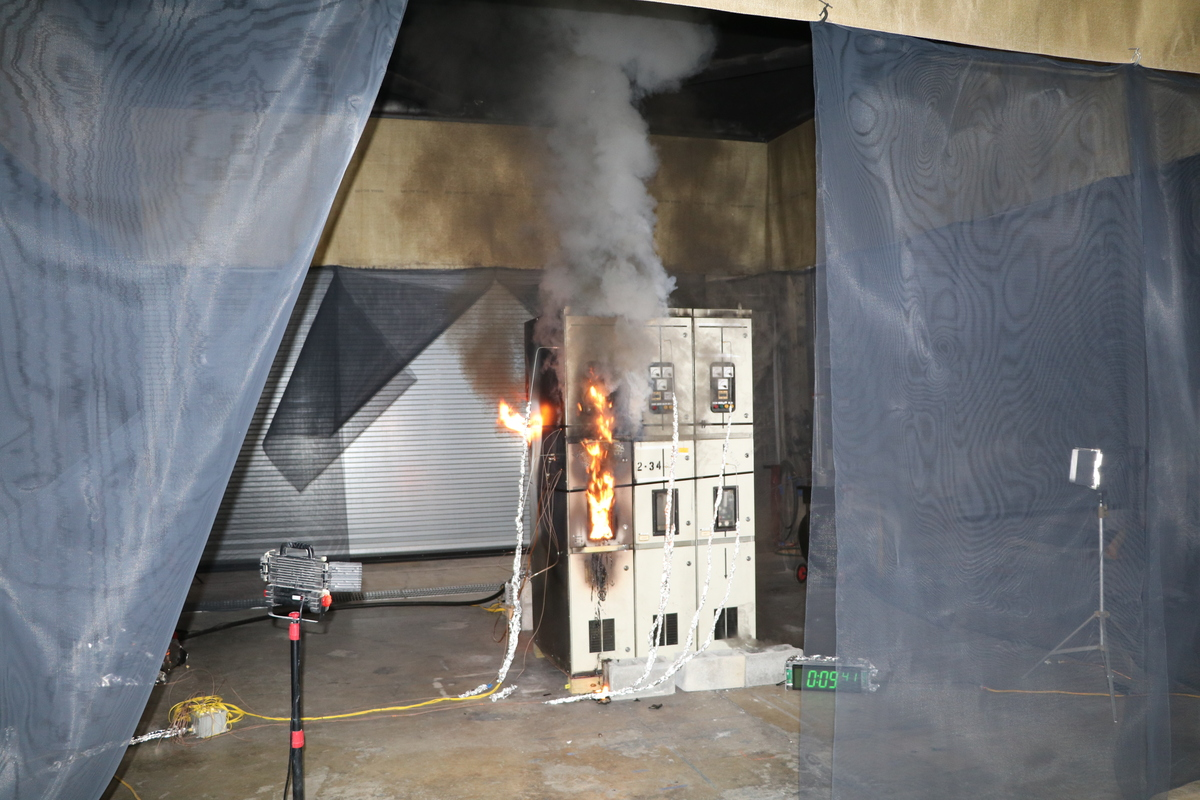
\includegraphics[height=2.50in]{../FIGURES/Test_33_9_min} \\ \vspace{0.1in}
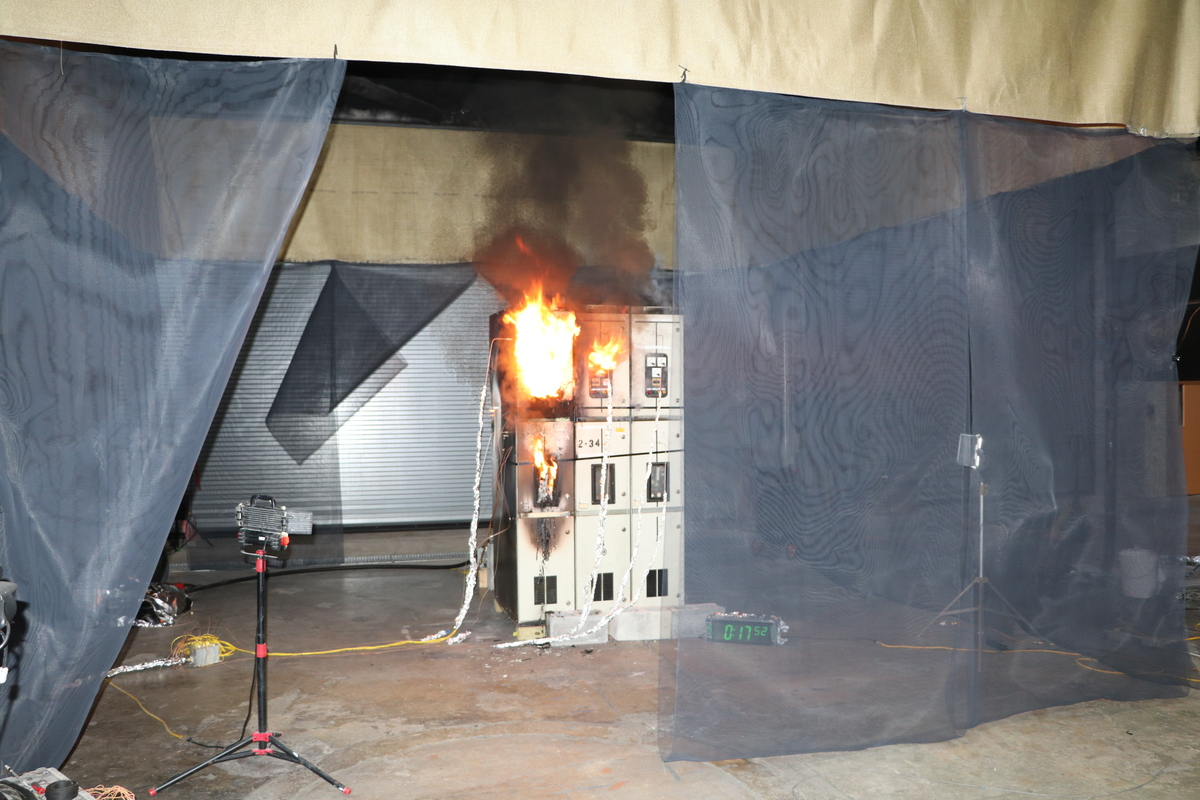
\includegraphics[height=2.50in]{../FIGURES/Test_33_17_min} \\ \vspace{0.1in}
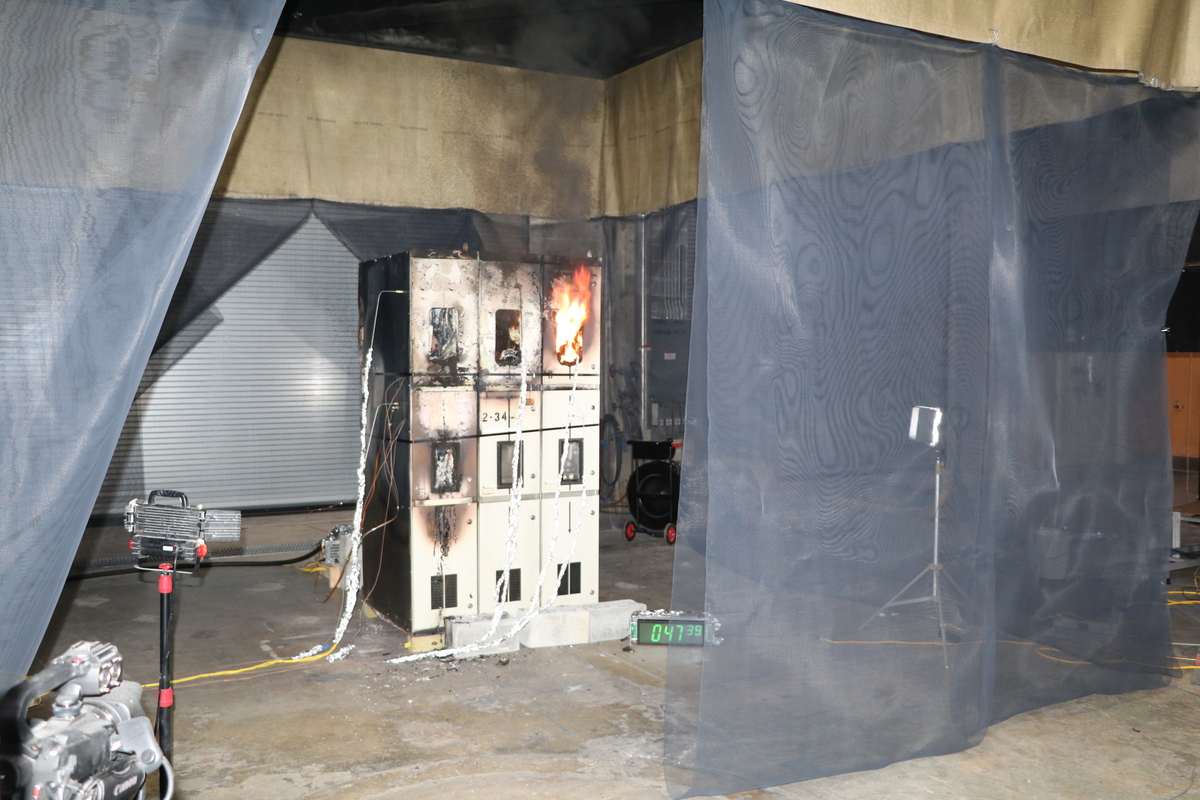
\includegraphics[height=2.50in]{../FIGURES/Test_33_47_min}
\caption[Photographs of Experiment~33]{Photographs of Experiment~33, 9~min, 17~min, and 47~min (top to bottom) after ignition of the burner which was located in the lower left compartment.}
\label{fig:Test_33_photos}
\end{figure}



\clearpage

\subsubsection{Experiment 34}

The fire in Exp.~33 consumed all of the combustibles in the upper compartments of the large enclosure. However, the breakers in the center and right columns remained intact. For Exp.~34, the burner was placed beneath the breaker on the right side of the enclosure (see Fig.~\ref{fig:Test_34_photos}) with the aim of measuring its HRR with no combustibles in the compartment above. The gas temperature in the compartment above reaches only approximately 400~$^\circ$C because there is no significant fire in this compartment, only the heat from the fire below.

\begin{figure}[!ht]
\begin{tabular*}{\textwidth}{l@{\extracolsep{\fill}}r}
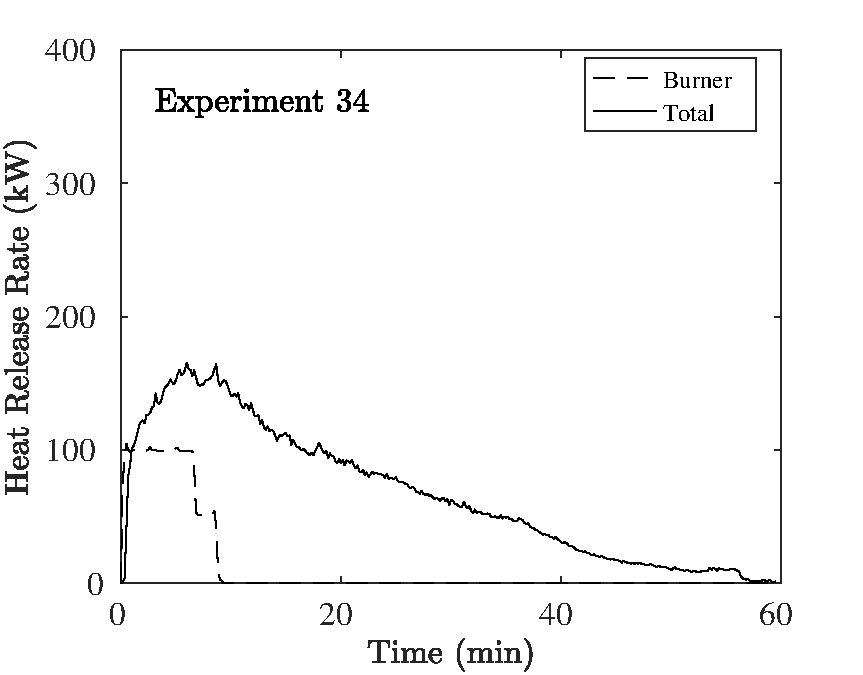
\includegraphics[height=2.2in]{../SCRIPT_FIGURES/Test_34_HRR} &
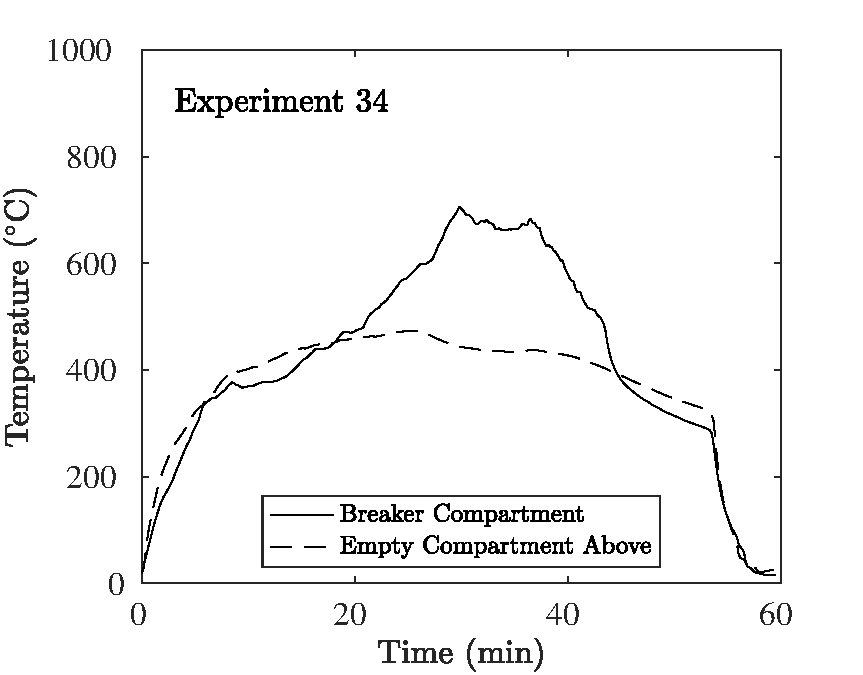
\includegraphics[height=2.2in]{../SCRIPT_FIGURES/Test_34_Gas_TC} \\
\multicolumn{2}{c}{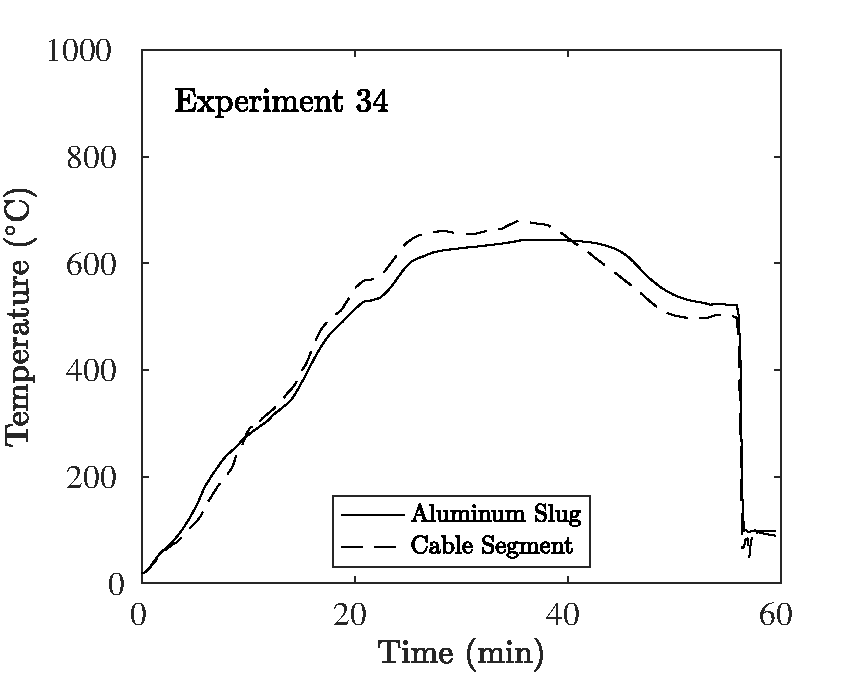
\includegraphics[height=2.2in]{../SCRIPT_FIGURES/Test_34_Slug_TC}}
\end{tabular*}
\caption[HRR and temperatures of Exp.~34]{Heat release rate (upper left), gas temperatures (upper right), and slug/cable temperatures (bottom) for Exp.~34. The curve labeled ``Burner'' in the upper left plot represents the ideal HRR based on natural gas flow, and ``Total'' is the HRR measured via oxygen-consumption calorimetry. The gas temperatures were recorded near the ceiling of the middle right compartment housing the breaker (``Breaker Compartment''), and the upper right compartment with the burned out remnants from Experiment~33 (''Empty Compartment Above''). In the bottom plot, the ``Aluminum Slug'' and thermoplastic ``Cable Segment'' were placed atop the breaker.}
\label{fig:Test_34}
\end{figure}

\begin{figure}[p]
\centering
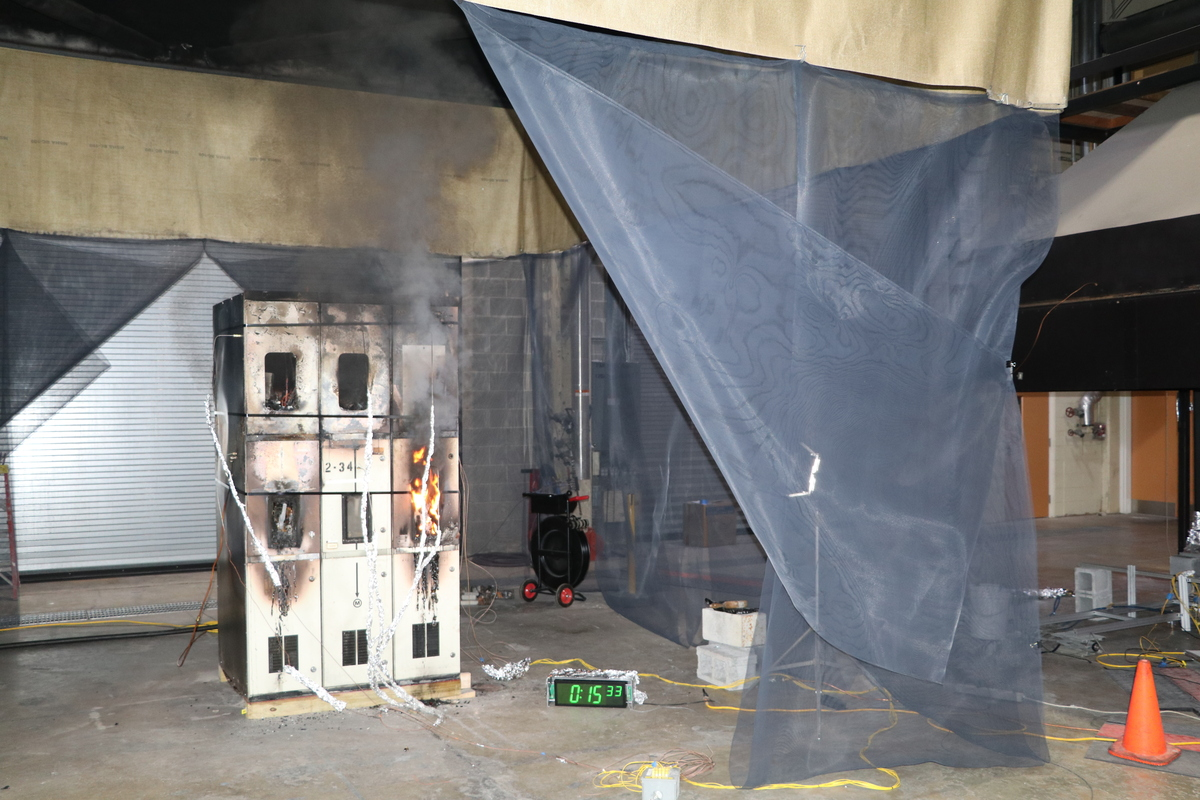
\includegraphics[height=2.50in]{../FIGURES/Test_34_15_min} \\ \vspace{0.1in}
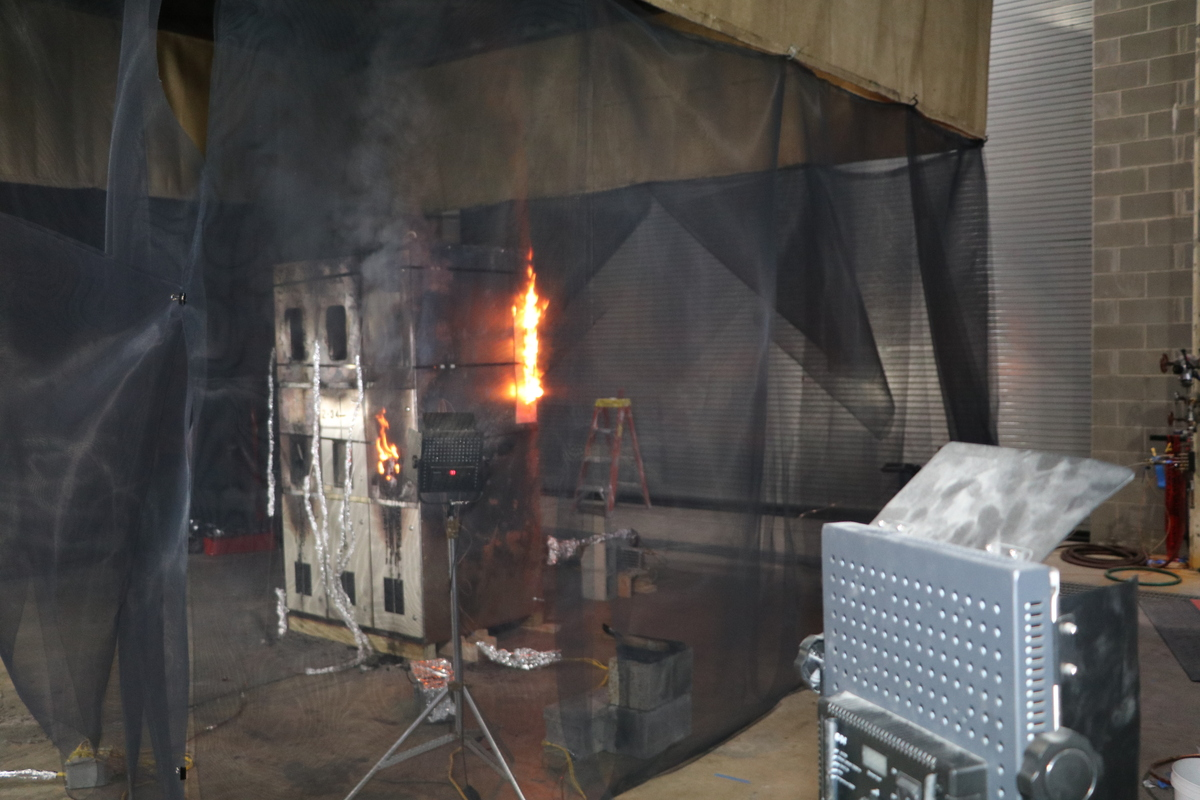
\includegraphics[height=2.50in]{../FIGURES/Test_34_30_min} \\ \vspace{0.1in}
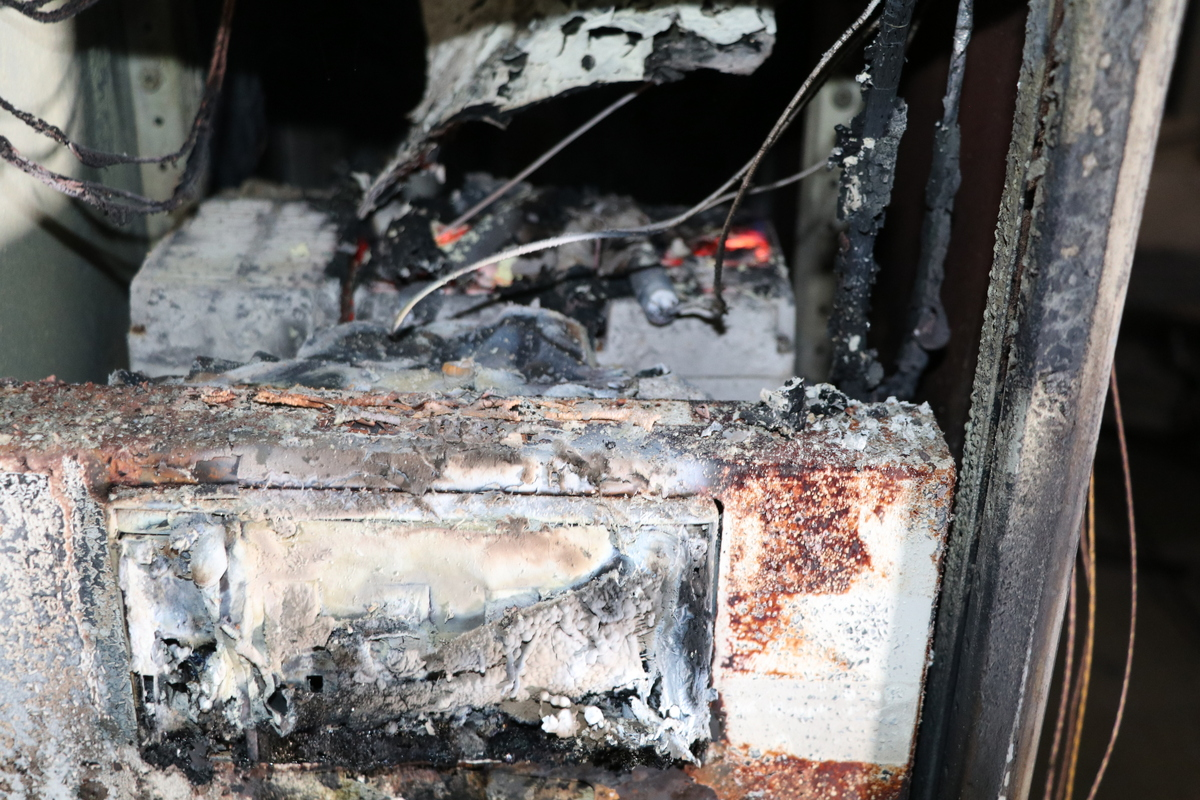
\includegraphics[height=2.50in]{../FIGURES/Test_34_60_min}
\caption[Photographs of Exp.~34]{Photographs of Exp.~34, 15~min, 30~min, and 60~min (top to bottom) after ignition of the burner which was located in the lower right compartment. The bottom photograph shows the breaker after the experiment continues to glow red due to the heat trapped within.}
\label{fig:Test_34_photos}
\end{figure}


\clearpage

\subsubsection{Experiment 35}

Figure~\ref{fig:Test_35} displays the HRR and gas/target temperatures for Exp.~35. Referring to Fig.~\ref{fig:Test_35_photos}, this experiment was conducted within the single-column ABB breaker enclosure, where the burner was positioned as in the previous experiments. The breaker ignited within 4~min at which time the burner was turned off. The total HRR dropped to about 50~kW at this time and then slowly increased as the fire spread from the breaker to the compartment above after approximately 18~min from the start of the experiment.

\begin{figure}[!ht]
\begin{tabular*}{\textwidth}{l@{\extracolsep{\fill}}r}
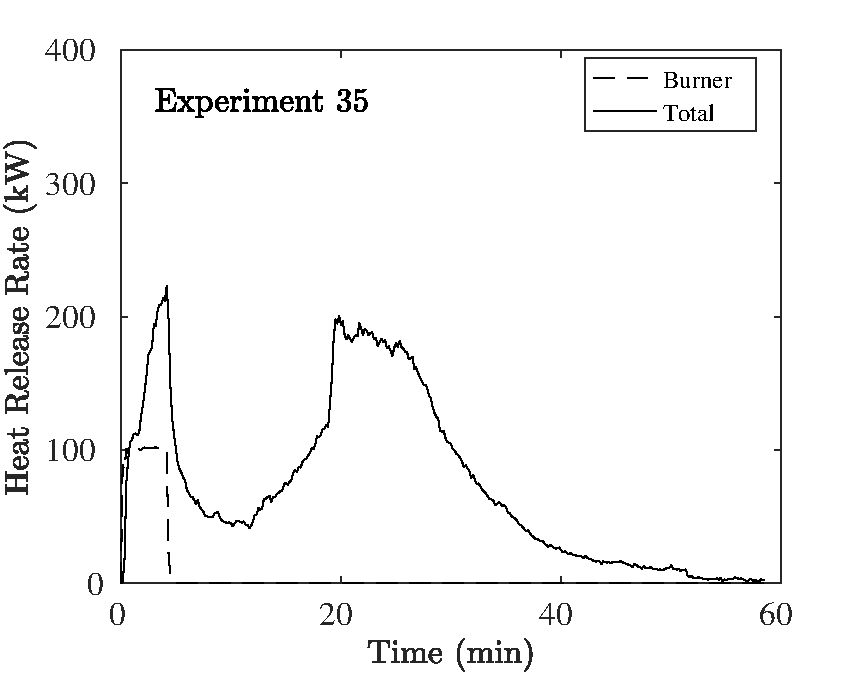
\includegraphics[height=2.40in]{../SCRIPT_FIGURES/Test_35_HRR} &
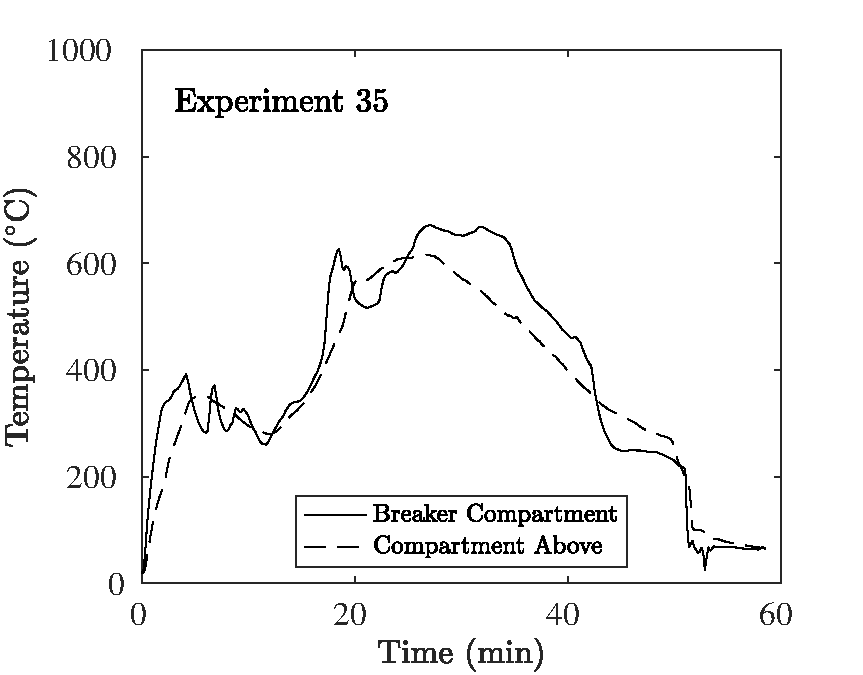
\includegraphics[height=2.40in]{../SCRIPT_FIGURES/Test_35_Gas_TC} \\
\multicolumn{2}{c}{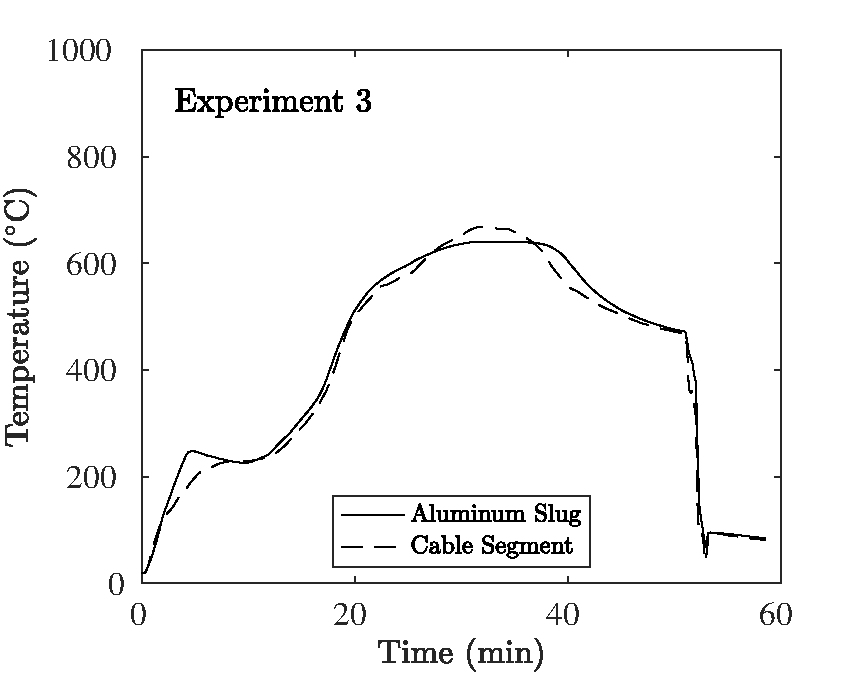
\includegraphics[height=2.40in]{../SCRIPT_FIGURES/Test_35_Slug_TC}}
\end{tabular*}
\caption[HRR and temperatures of Exp.~35]{Heat release rate (upper left), gas temperatures (upper right), and slug/cable temperatures (bottom) for Exp.~35. The curve labeled ``Burner'' in the upper left plot represents the ideal HRR based on natural gas flow, and ``Total'' is the HRR measured via oxygen-consumption calorimetry. The gas temperatures were recorded near the ceiling of the middle compartment housing the breaker (``Breaker Compartment''), and the upper compartment filled with miscellaneous wiring and plastics (''Compartment Above''). In the bottom plot, the ``Aluminum Slug'' and thermoplastic ``Cable Segment'' were placed atop the breaker.}
\label{fig:Test_35}
\end{figure}

\begin{figure}[p]
\centering
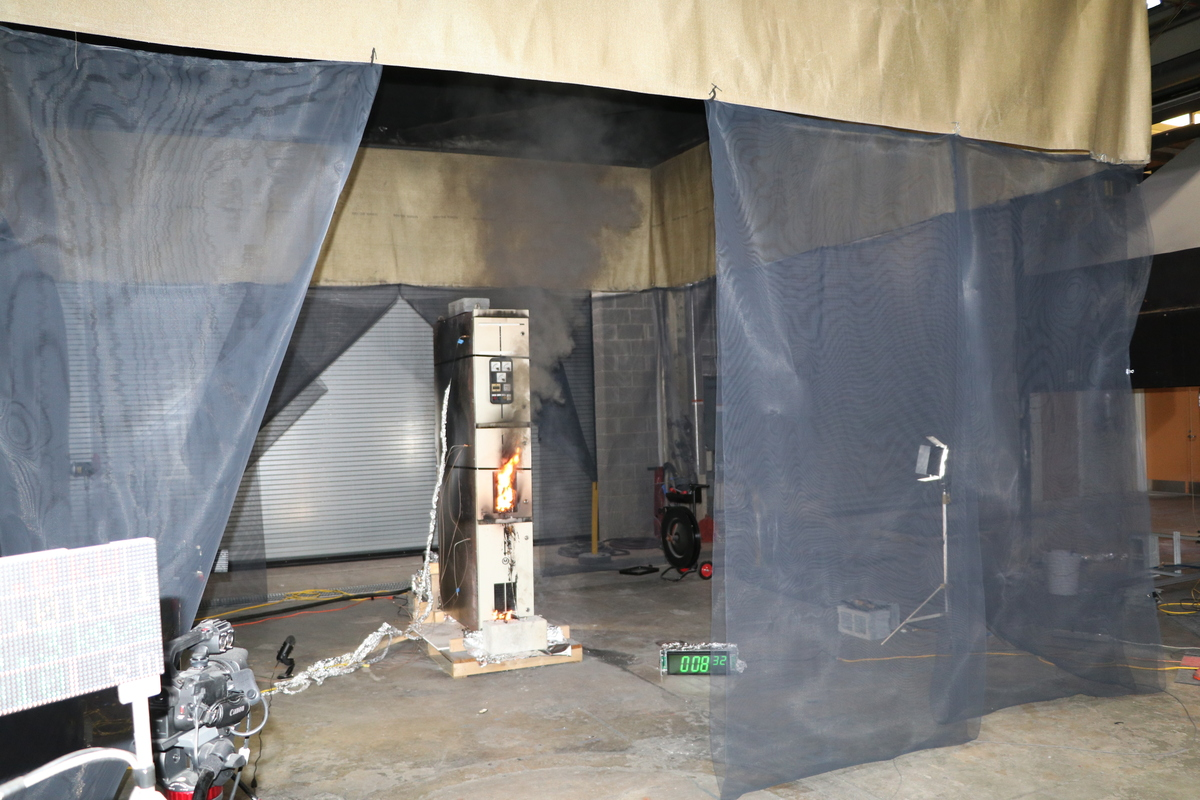
\includegraphics[height=2.50in]{../FIGURES/Test_35_8_min} \\ \vspace{0.1in}
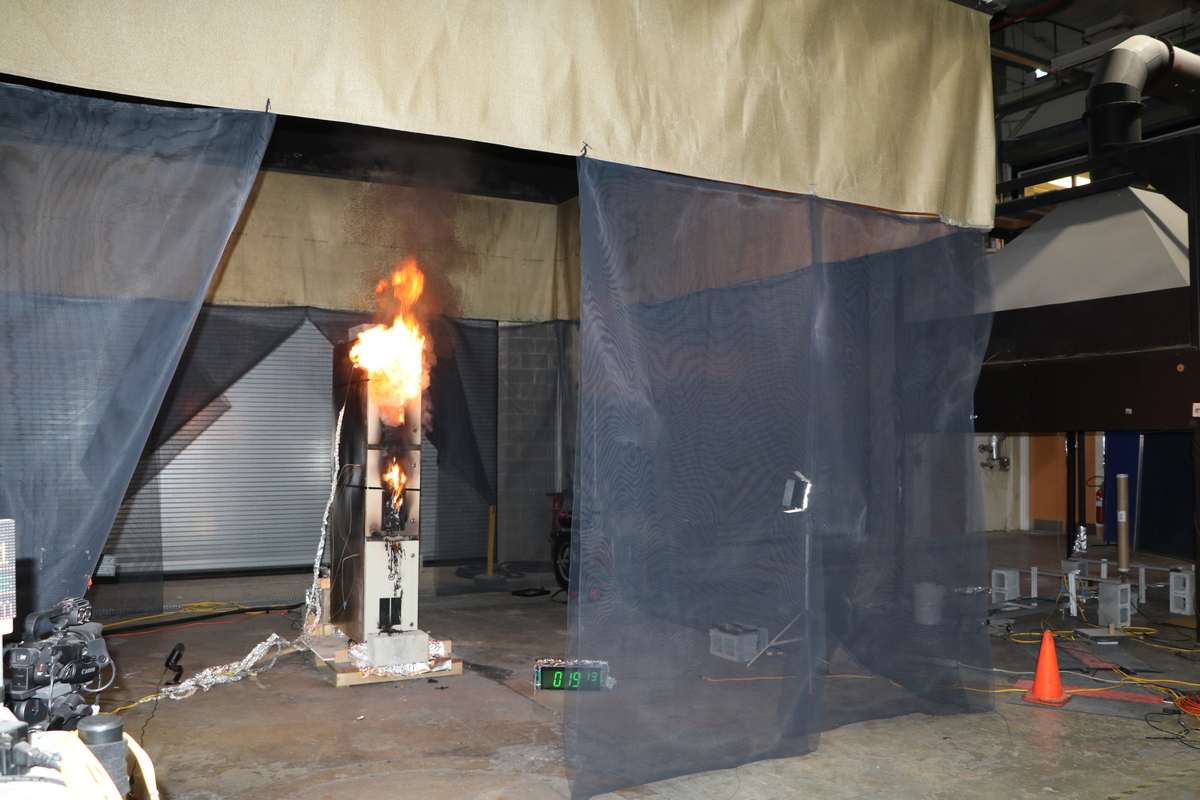
\includegraphics[height=2.50in]{../FIGURES/Test_35_19_min} \\ \vspace{0.1in}
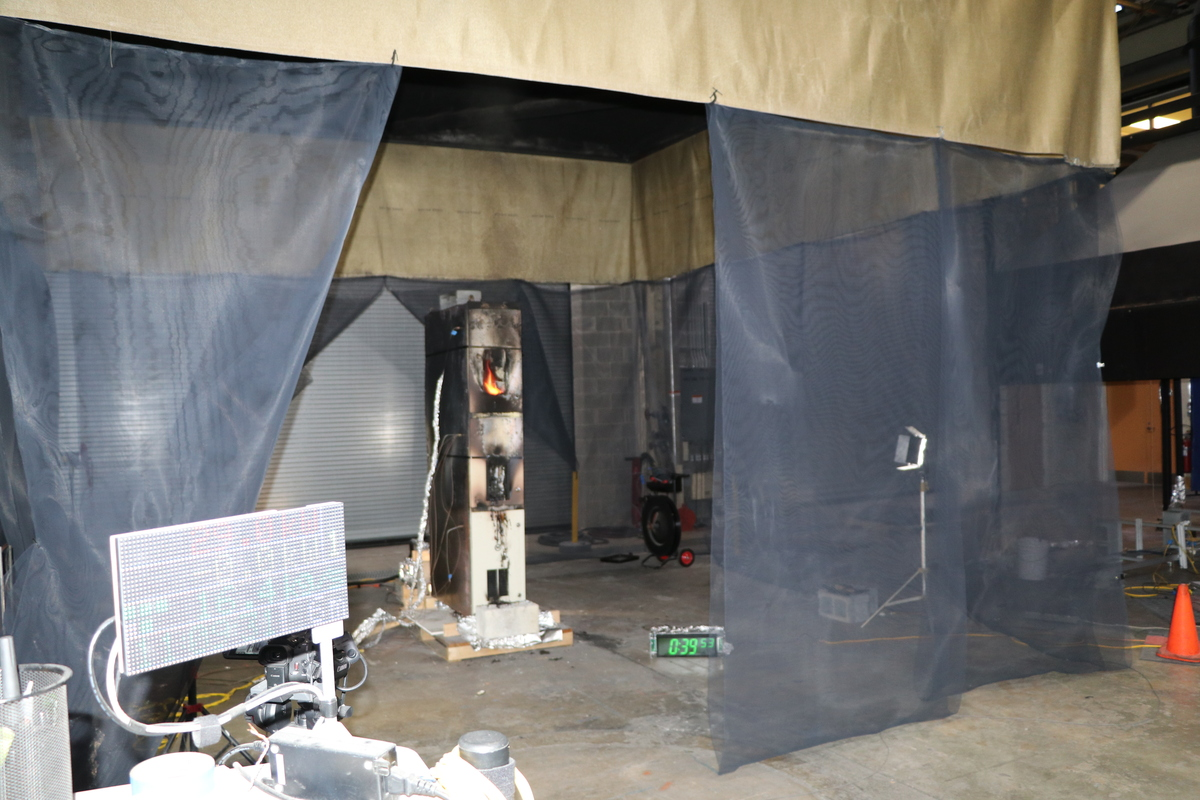
\includegraphics[height=2.50in]{../FIGURES/Test_35_39_min}
\caption[Photographs of Exp.~35]{Photographs of Exp.~35, 8~min, 19~min, and 39~min (top to bottom) after ignition of the burner which was located in the lower compartment.}
\label{fig:Test_35_photos}
\end{figure}


\clearpage

\subsubsection{Experiment 40}

Figure~\ref{fig:Test_40} displays the HRR and key temperatures of Experiment~40. Referring to Fig.~\ref{fig:Test_40_photos}, the gas burner was positioned within the lower right compartment of a Westinghouse low-voltage breaker enclosure. Breakers occupied the two compartments above, and the compartment above that was filled with approximately 0.8~kg of panel wire. A 30~cm (12~in) wide tray containing 12 thermoplastic cables was placed approximately 30~cm (12~in) above the top of the enclosure. Thermocouples were inserted into three cables within the tray, and instrumented aluminum rods (``slugs'') were placed alongside the instrumented cables. A single sheathed thermocouple was placed at the front of each compartment. All doors on the left side of the enclosure remained closed during the experiment except the one containing the burner.

\begin{figure}[!ht]
\begin{tabular*}{\textwidth}{l@{\extracolsep{\fill}}r}
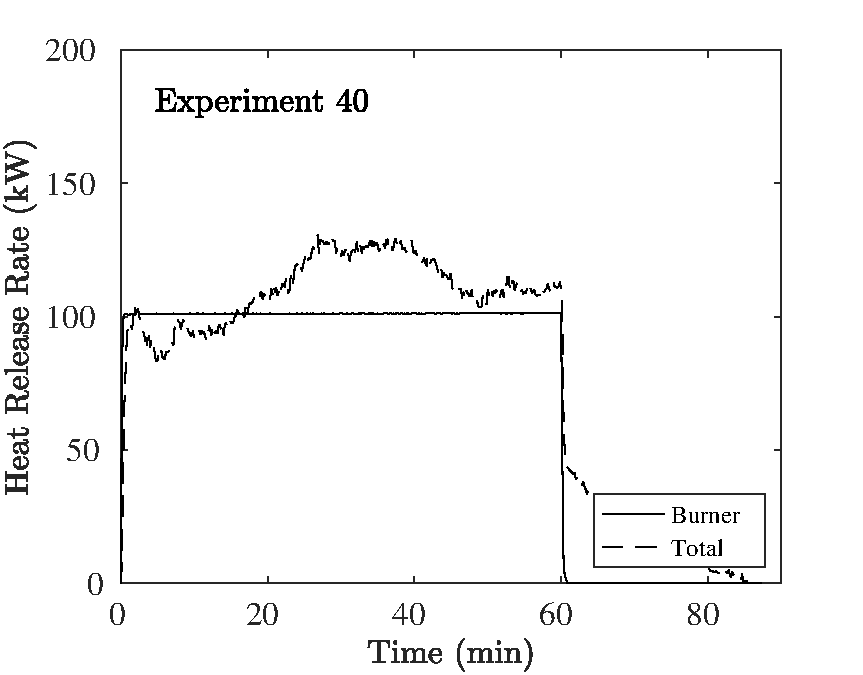
\includegraphics[height=2.2in]{../SCRIPT_FIGURES/Test_40_Plot_1} &
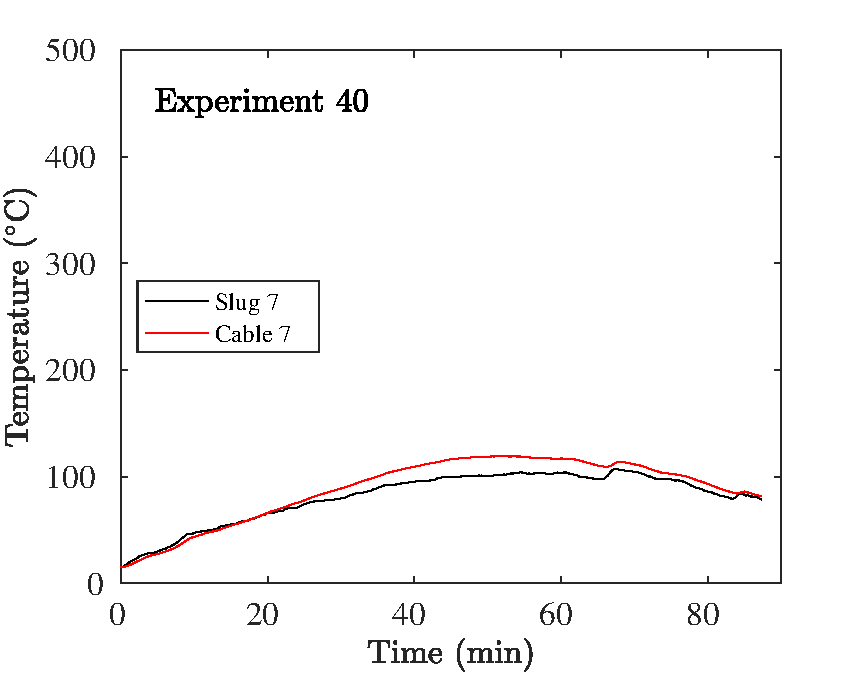
\includegraphics[height=2.2in]{../SCRIPT_FIGURES/Test_40_Plot_2} \\
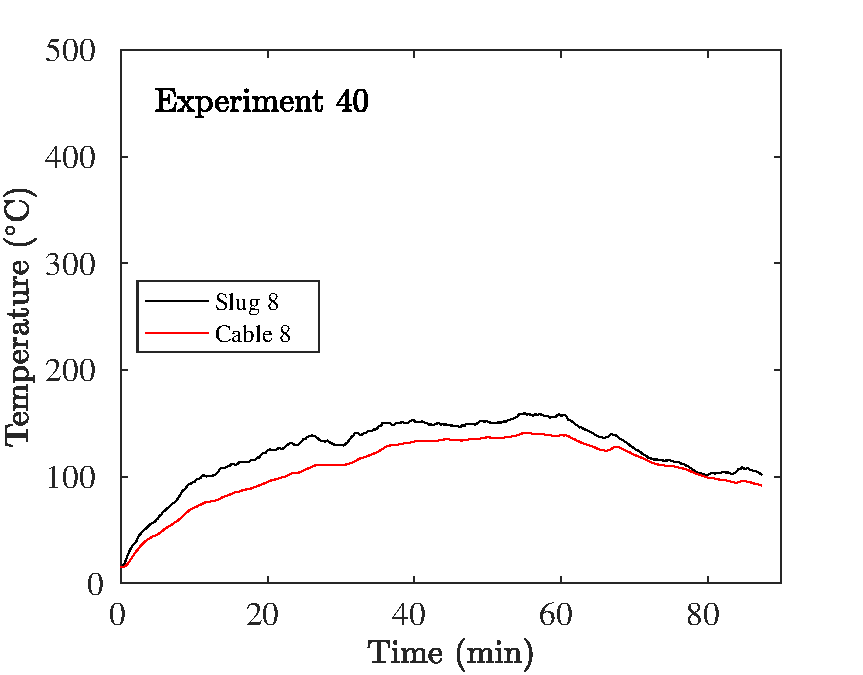
\includegraphics[height=2.2in]{../SCRIPT_FIGURES/Test_40_Plot_3} &
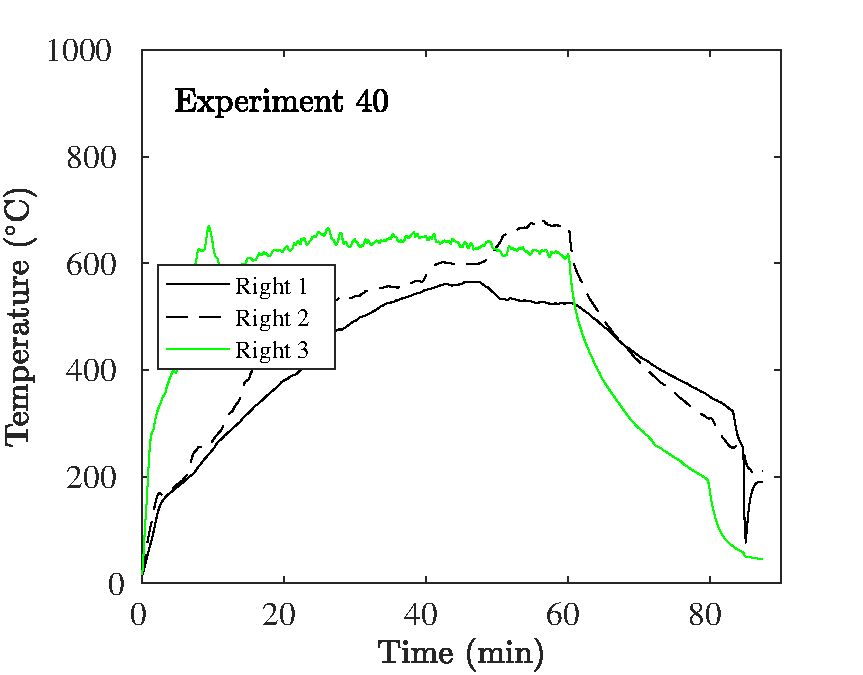
\includegraphics[height=2.2in]{../SCRIPT_FIGURES/Test_40_Plot_5}
\end{tabular*}
\caption[HRR and temperatures of Exp.~40]{The curve labeled ``Burner'' in the upper left plot represents the ideal HRR based on natural gas flow, and ``Total'' is the HRR measured via oxygen-consumption calorimetry. The curves labeled ``Slug X'' and ``Cable X'' are temperatures of cables and aluminum  rods (slugs) in the cable tray above the enclosure. All were placed above the location of the fire, but those labeled with a 7 were to the rear of the tray; 8 to the front. The gas temperatures shown in the lower right plot refer to the lower breaker compartment (``Right 3''), upper breaker (``Right 2''), and top compartment with panel wire (``Right 1''). }
\label{fig:Test_40}
\end{figure}

\begin{figure}[p]
\centering
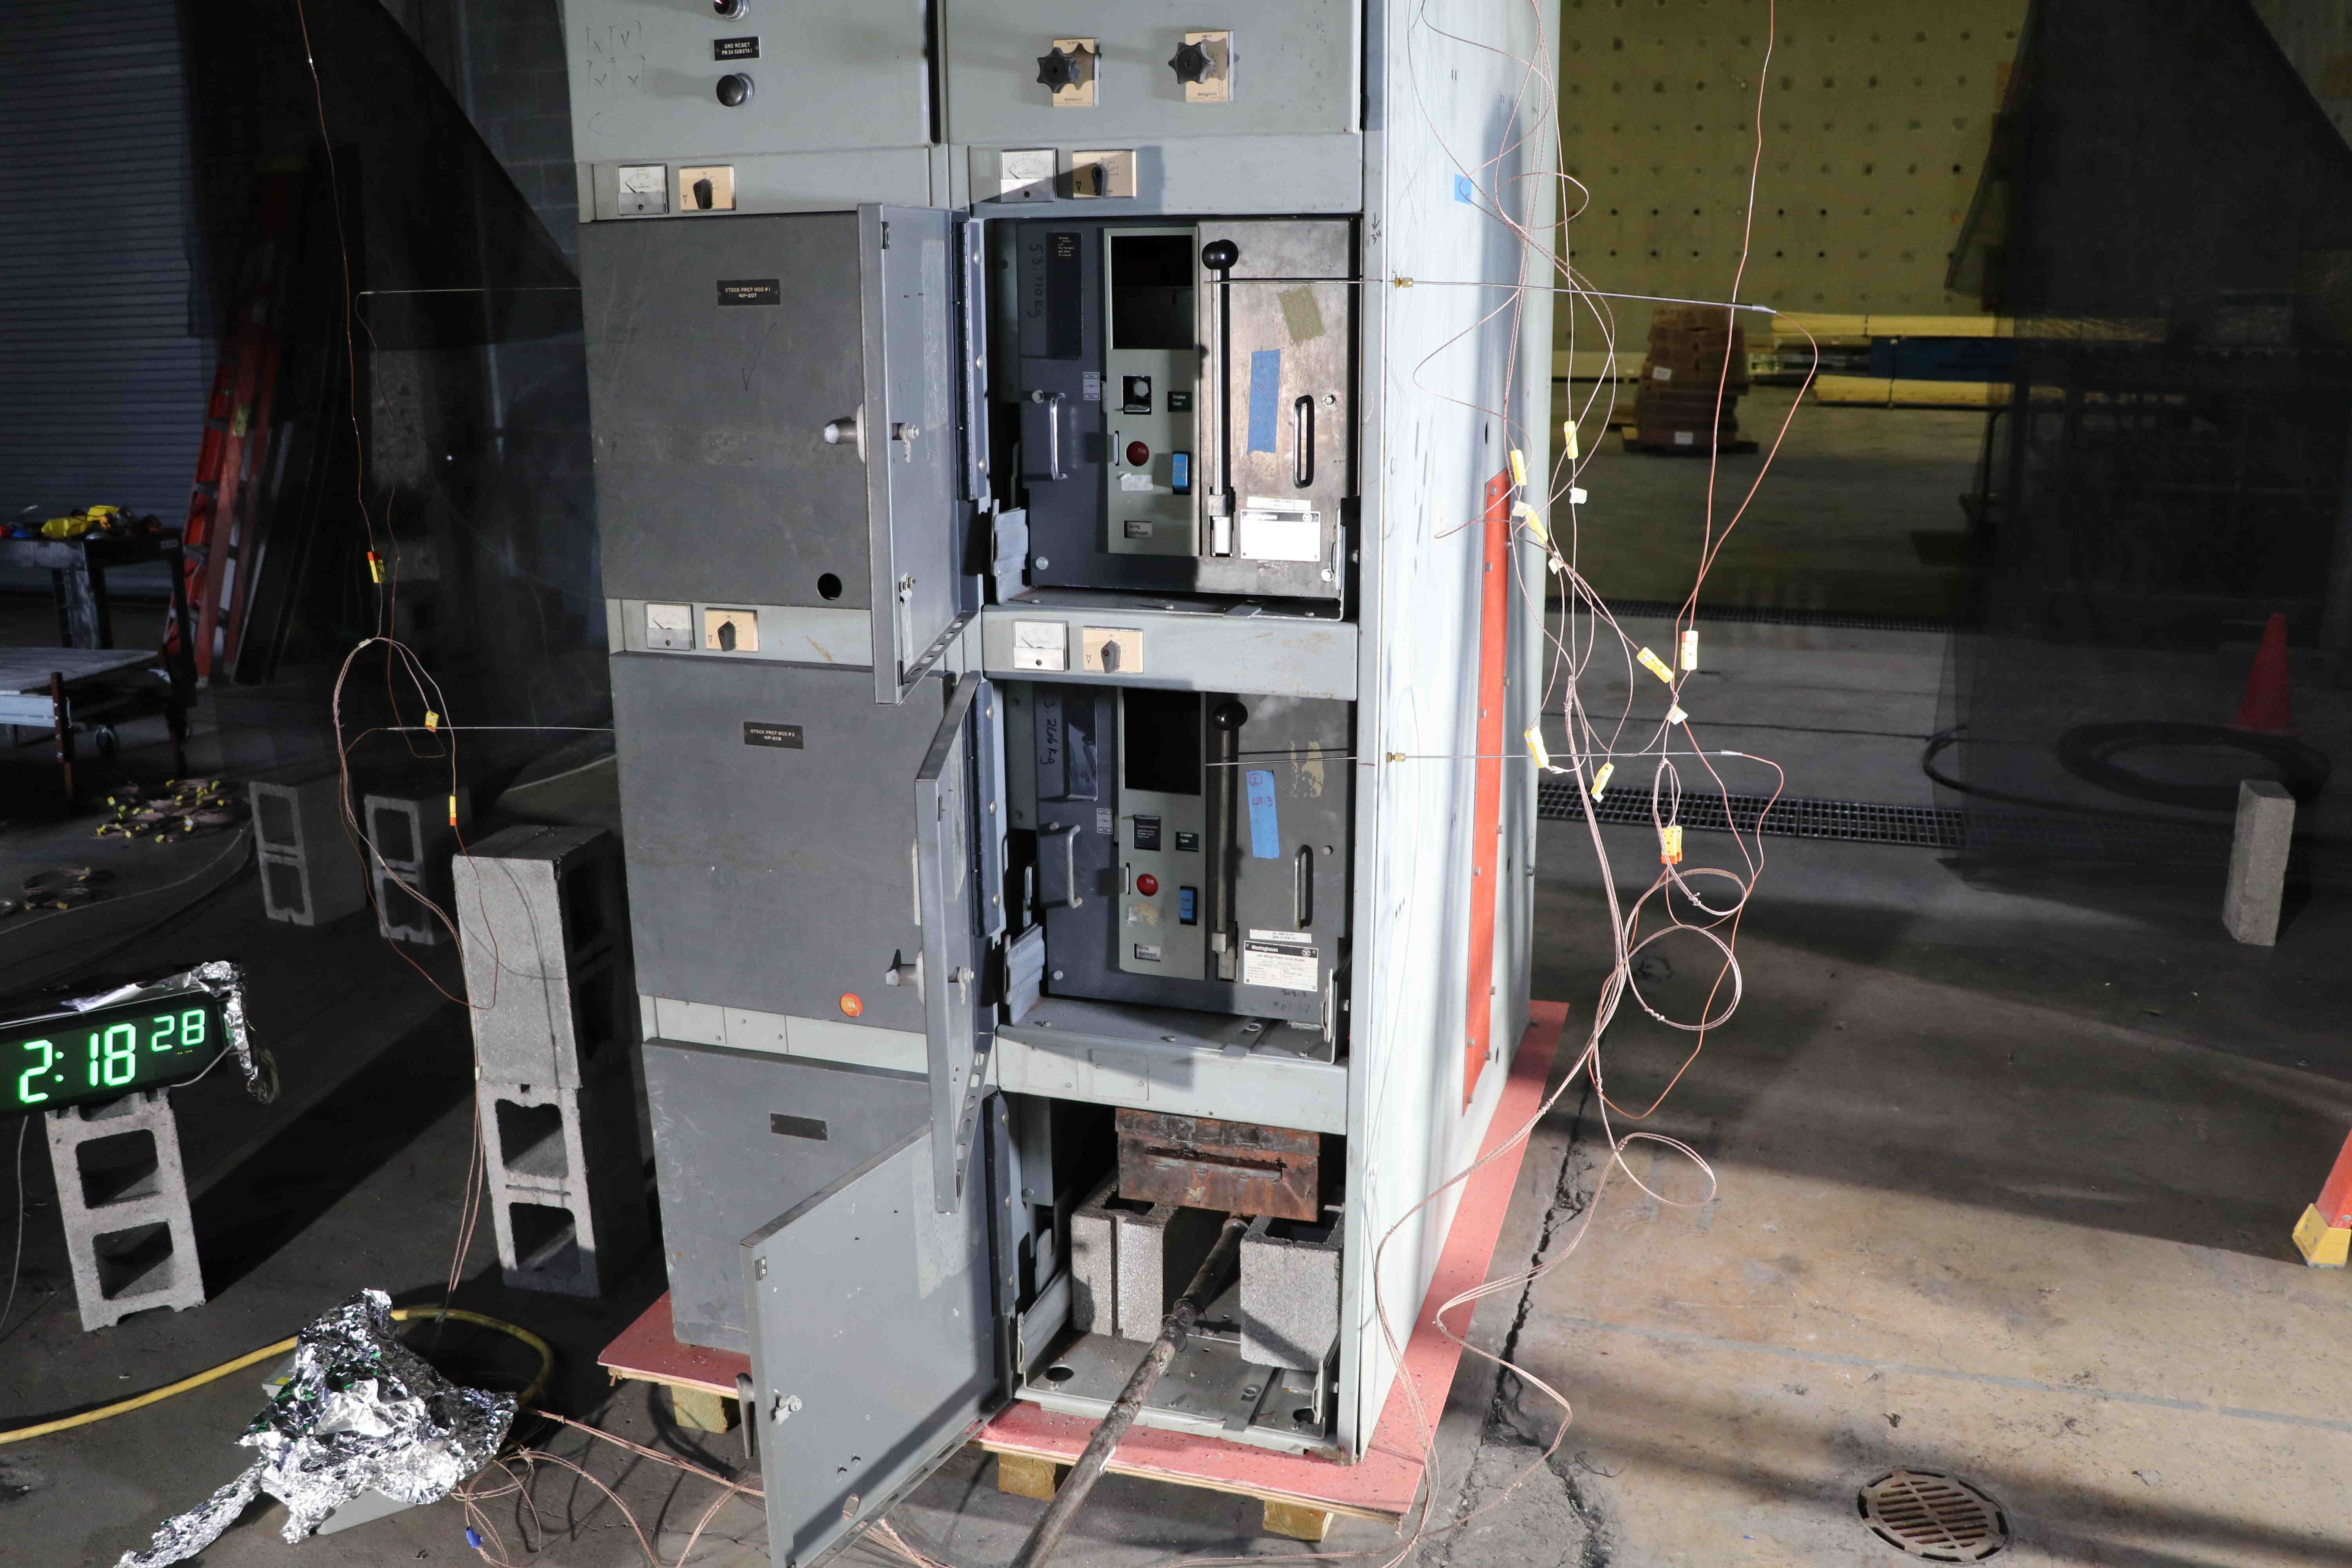
\includegraphics[height=2.50in]{../FIGURES/Test_40_setup} \\ \vspace{0.1in}
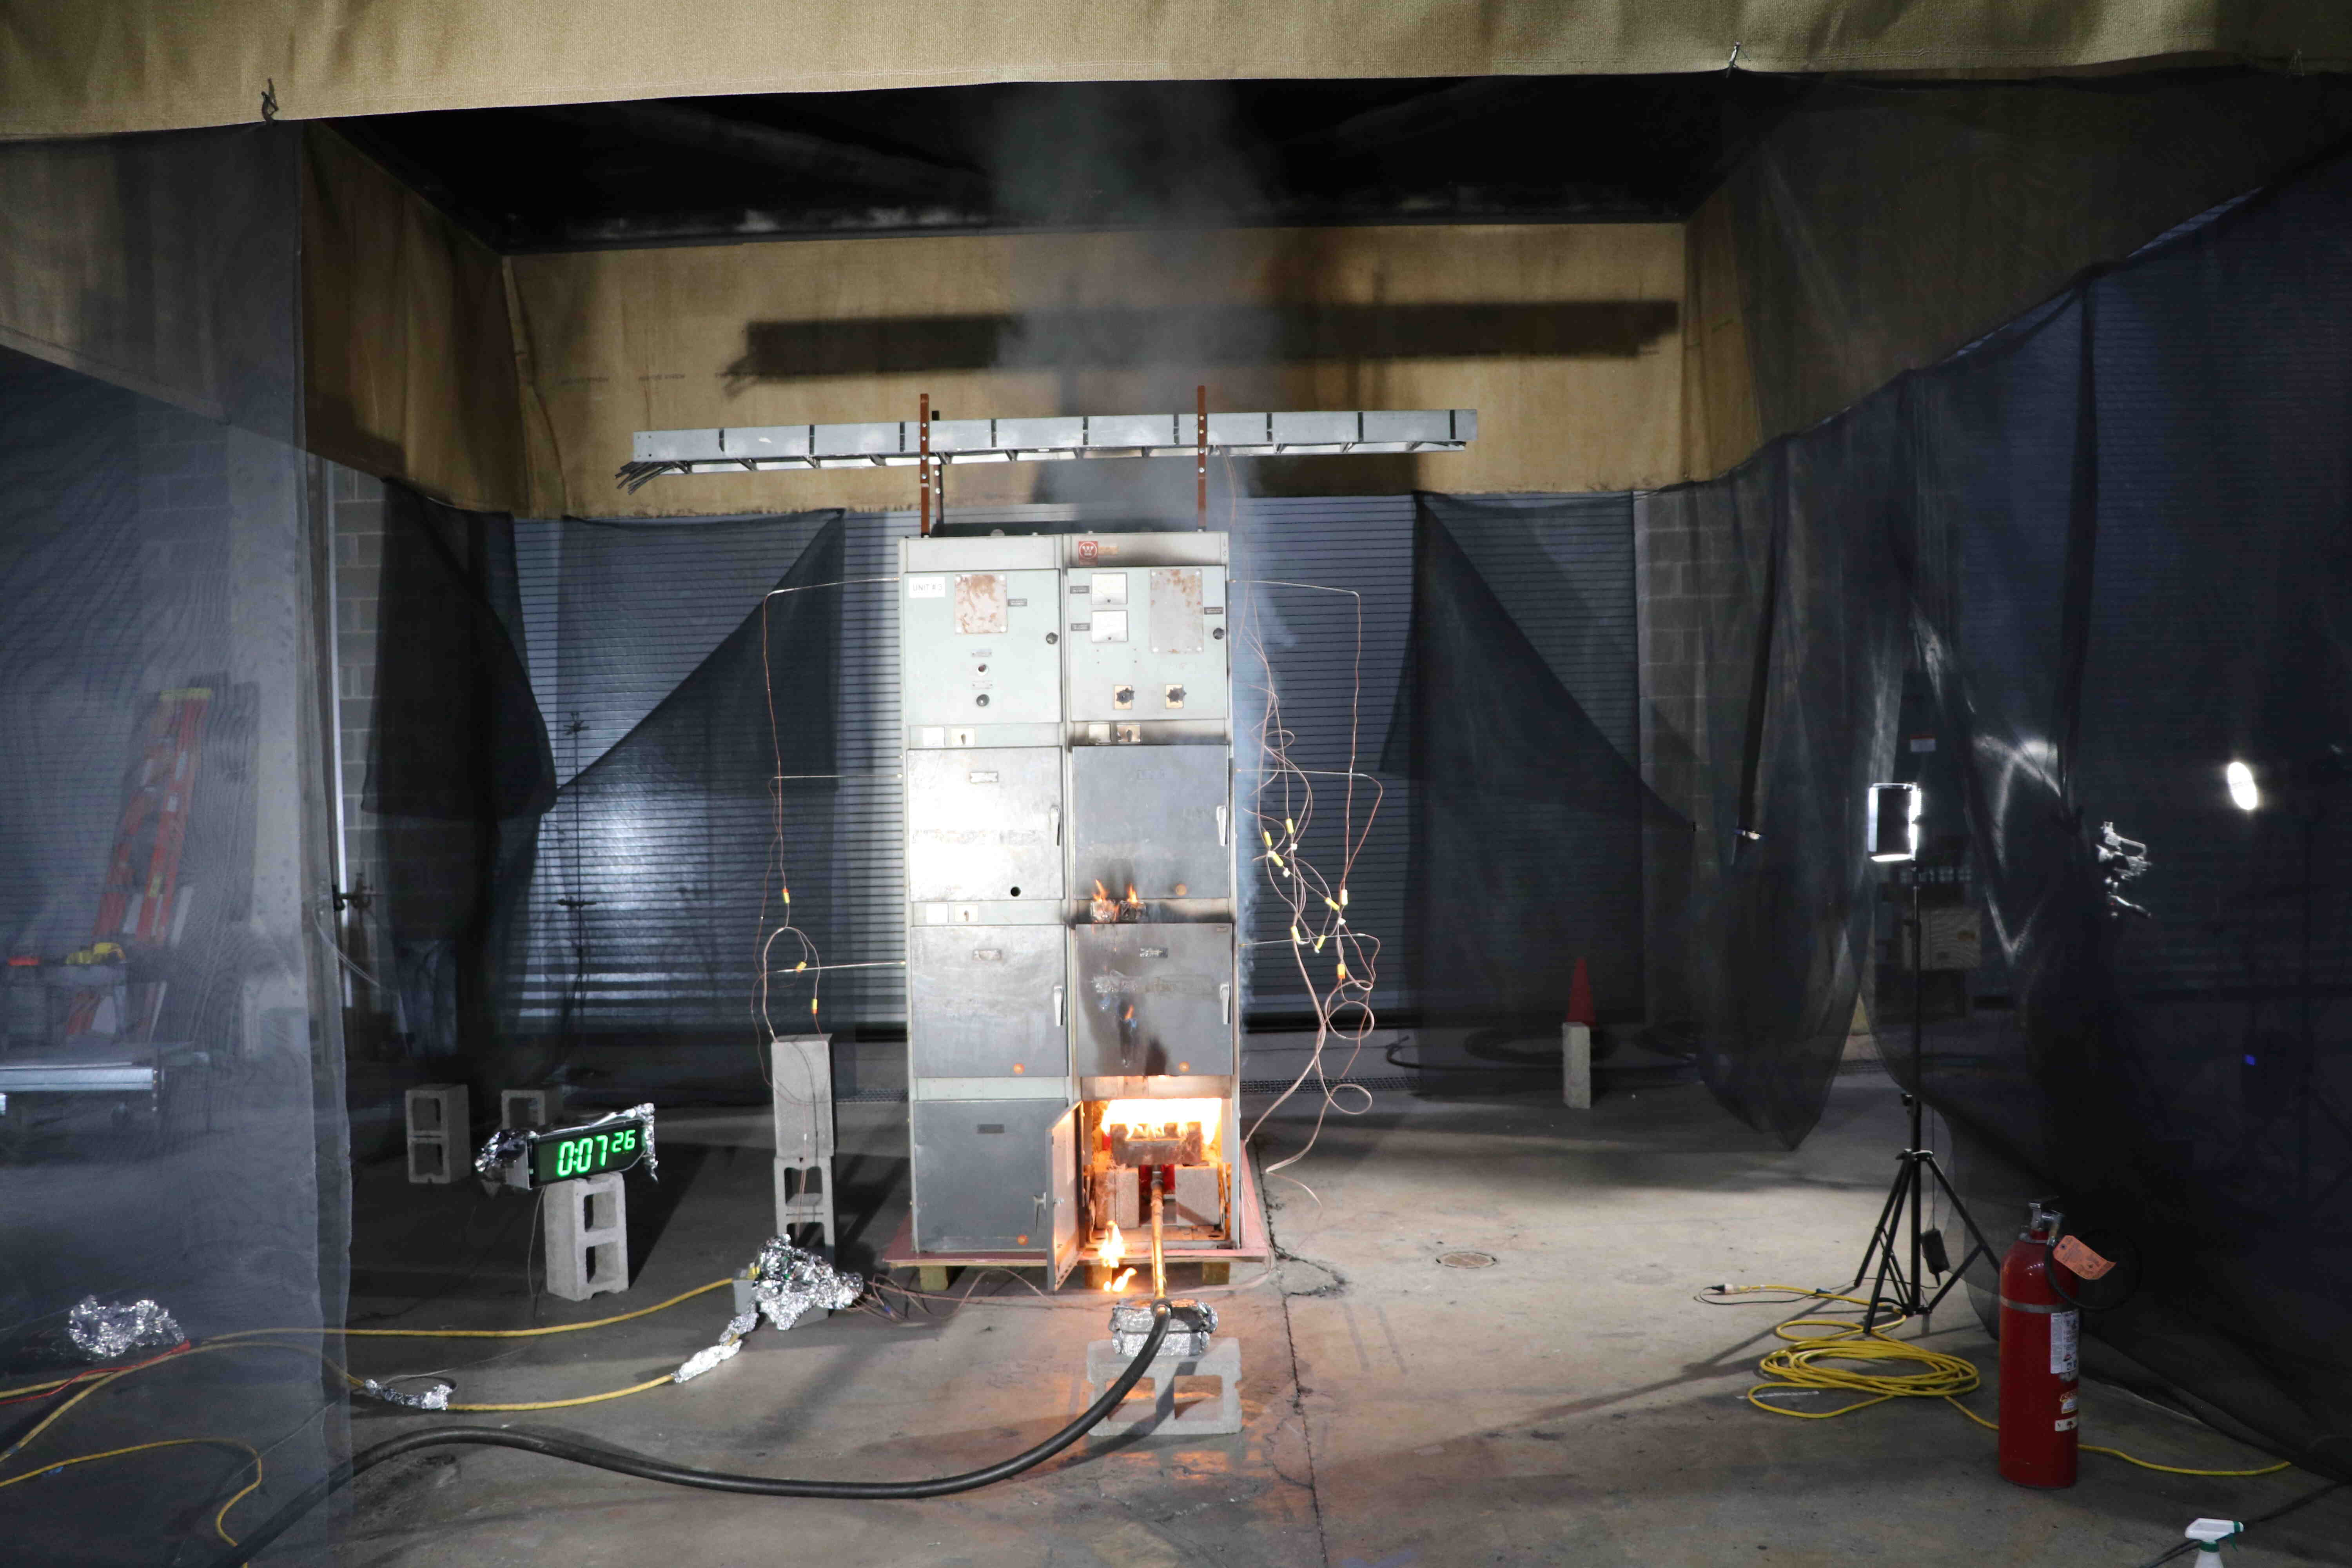
\includegraphics[height=2.50in]{../FIGURES/Test_40_7_min_26_s} \\ \vspace{0.1in}
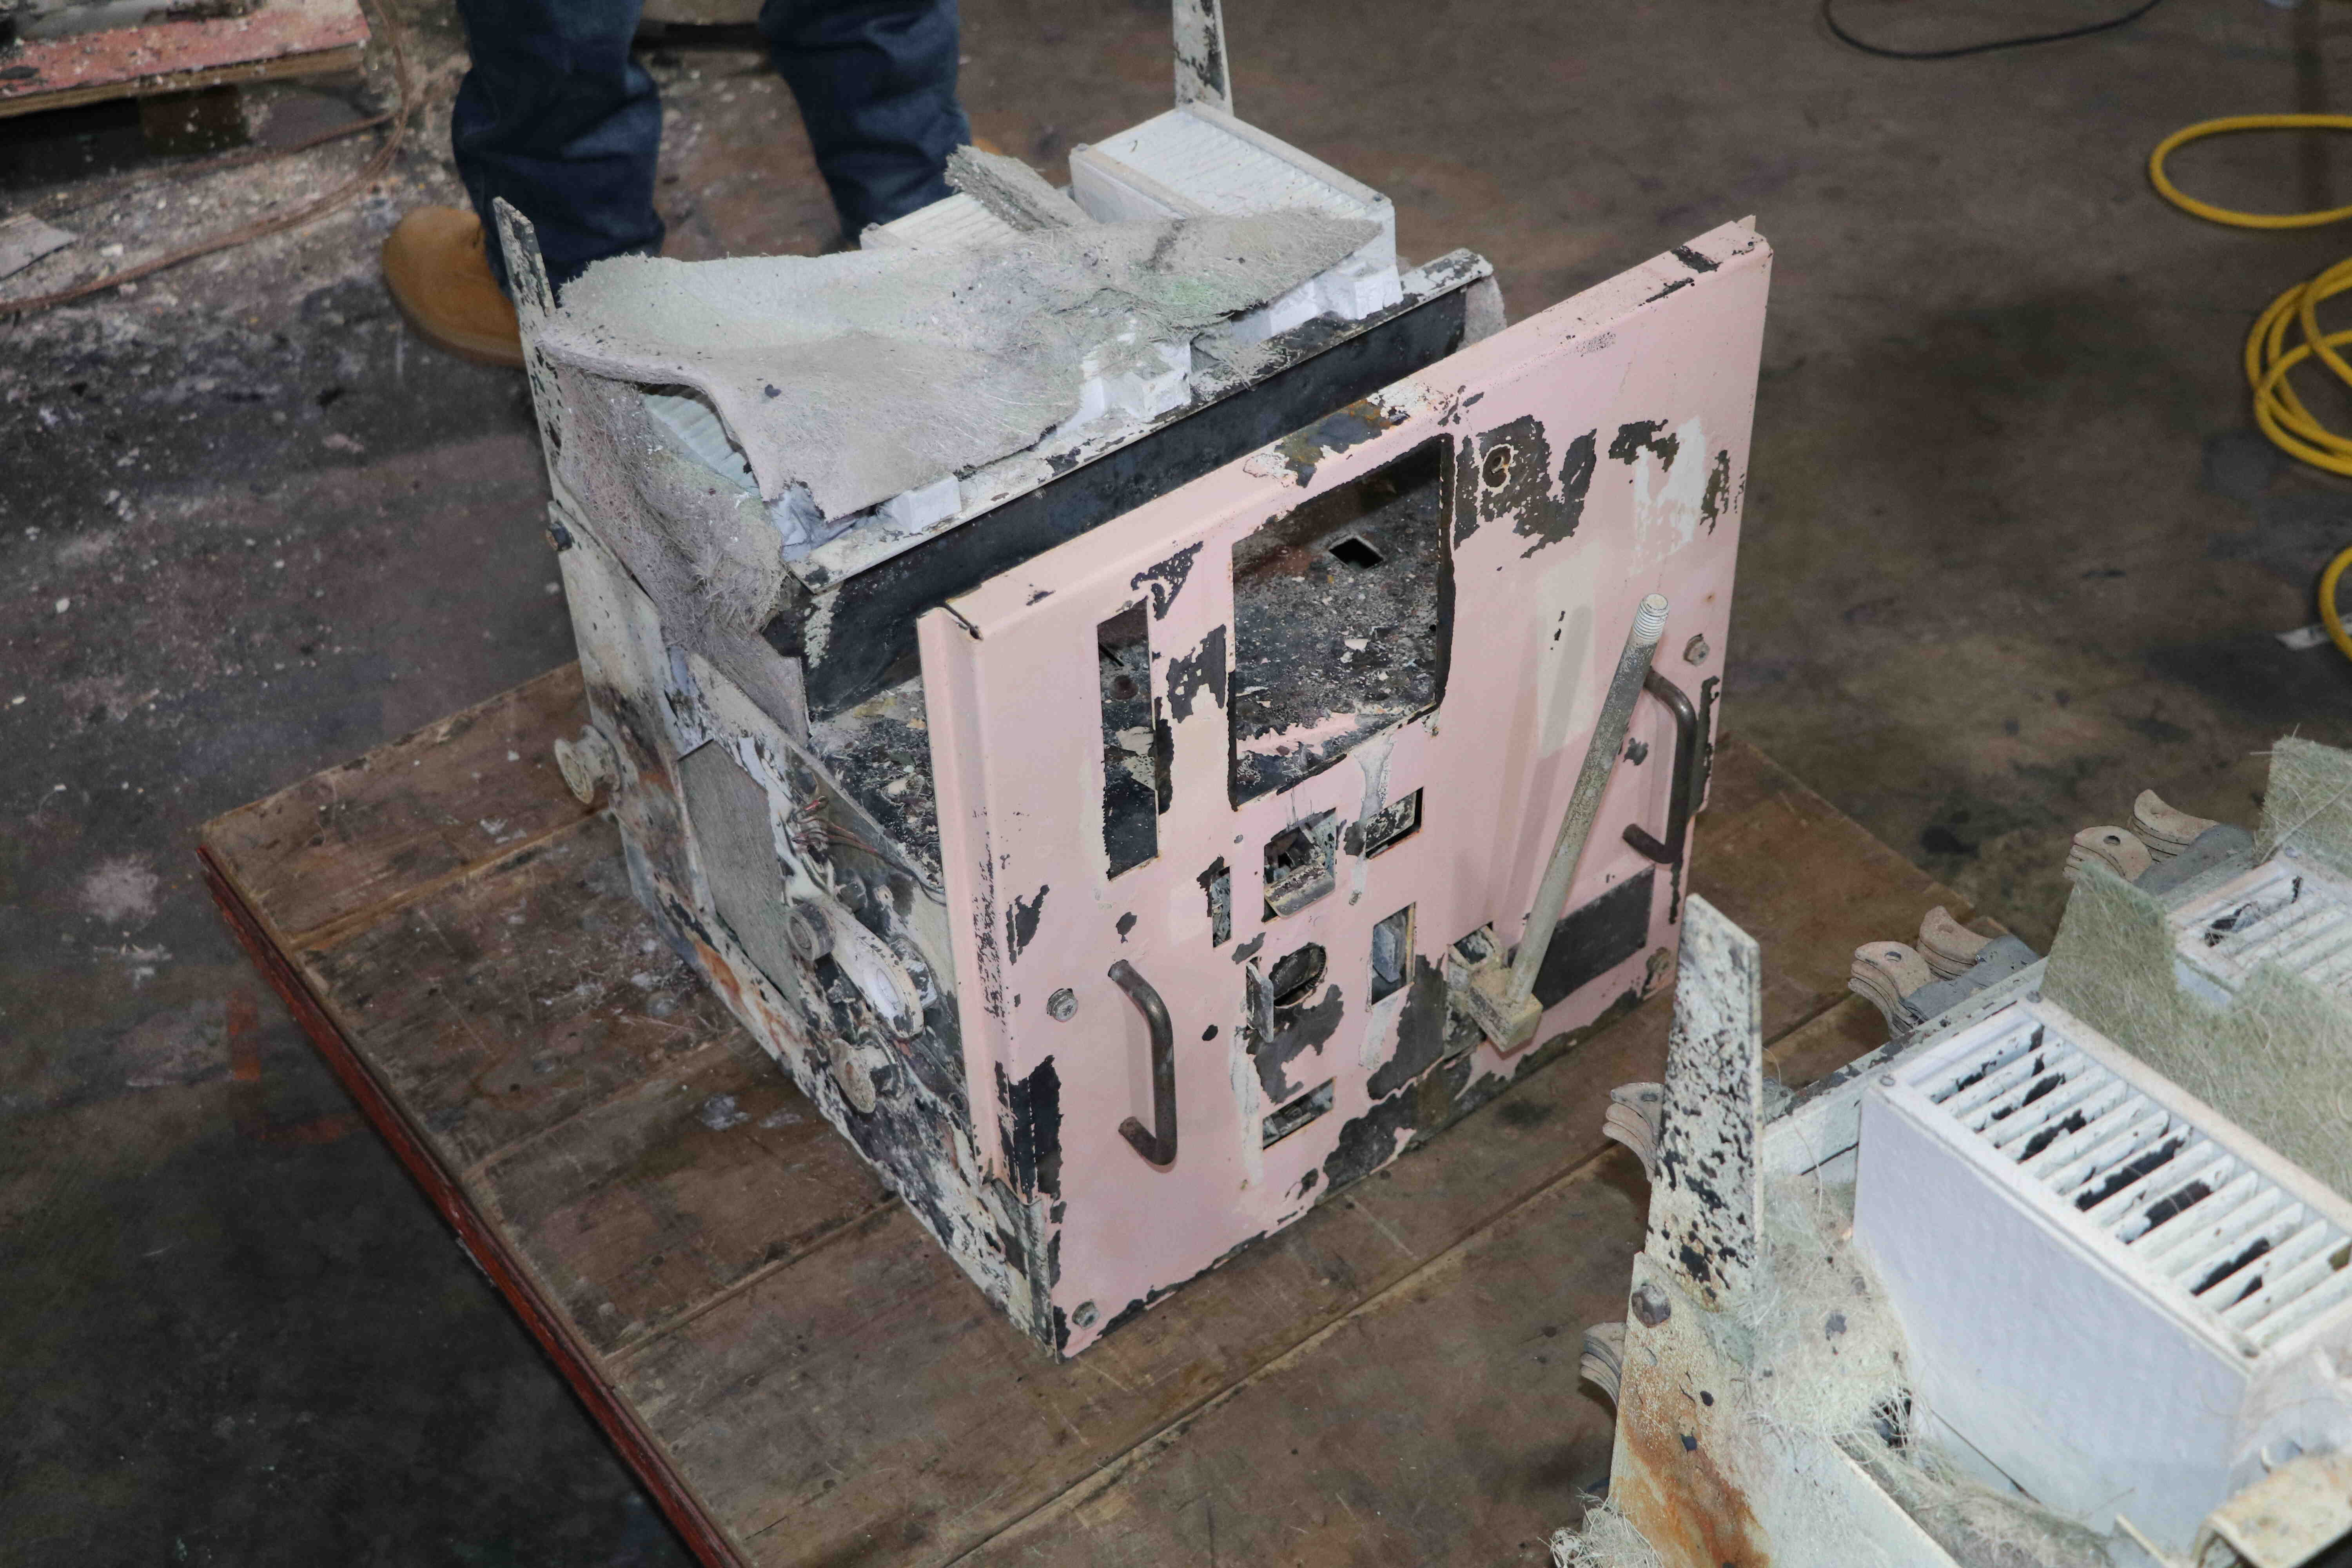
\includegraphics[height=2.50in]{../FIGURES/Test_40_breaker}
\caption[Photographs of Experiment~40]{Photographs of Experiment~40. (Top) The burner in position below the breaker. (Middle) The fire at 7~min, 26~s after ignition. (Bottom) The breaker after the experiment.}
\label{fig:Test_40_photos}
\end{figure}


\clearpage

\subsubsection{Experiment 41}

Figure~\ref{fig:Test_41} displays the HRR and key temperatures of Experiment~41. Referring to Fig.~\ref{fig:Test_41_photos}, the gas burner was positioned within the lower left compartment of a Westinghouse low-voltage breaker enclosure. Breakers occupied the two compartments above, and the compartment above that was filled with approximately 1.0~kg of panel wire. A 30~cm (12~in) wide tray containing 12 thermoplastic cables was placed approximately 30~cm (12~in) above the top of the enclosure. Thermocouples were inserted into three cables within the tray, and instrumented aluminum rods (``slugs'') were placed alongside the instrumented cables. A single sheathed thermocouple was placed at the front of each compartment. All doors on the left side of the enclosure remained open during the experiment.

\begin{figure}[!ht]
\begin{tabular*}{\textwidth}{l@{\extracolsep{\fill}}r}
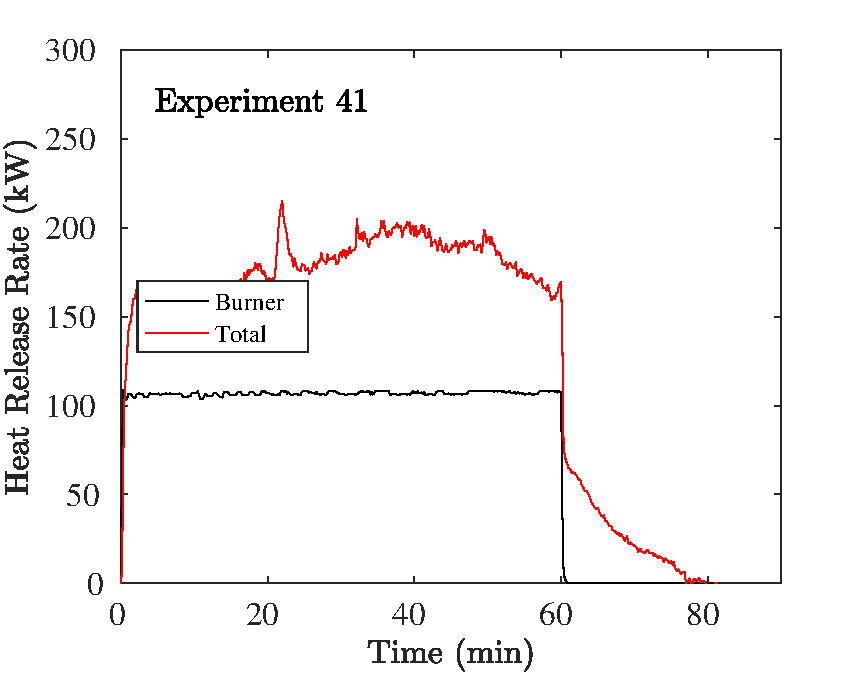
\includegraphics[height=2.2in]{../SCRIPT_FIGURES/Test_41_Plot_1} &
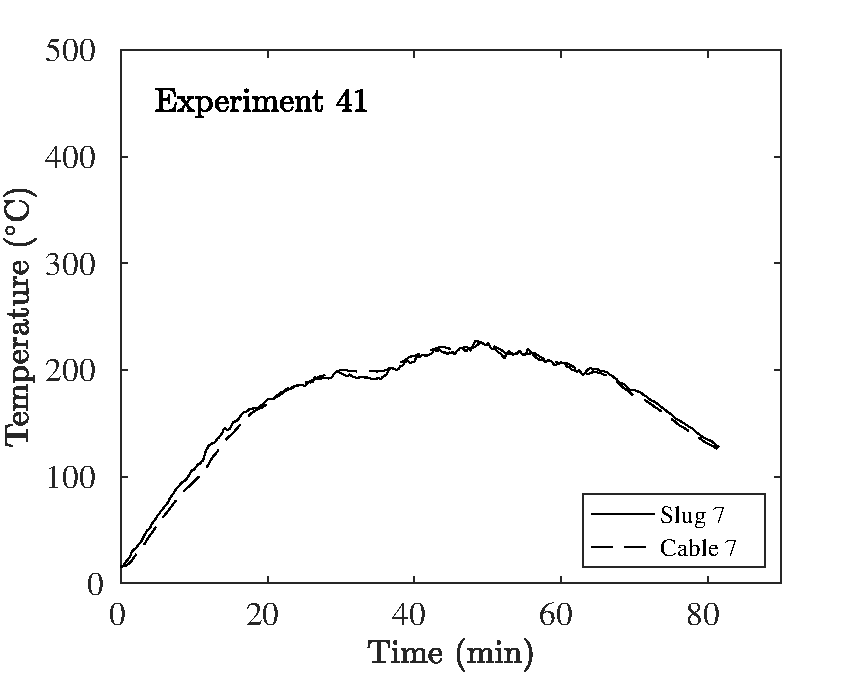
\includegraphics[height=2.2in]{../SCRIPT_FIGURES/Test_41_Plot_2} \\
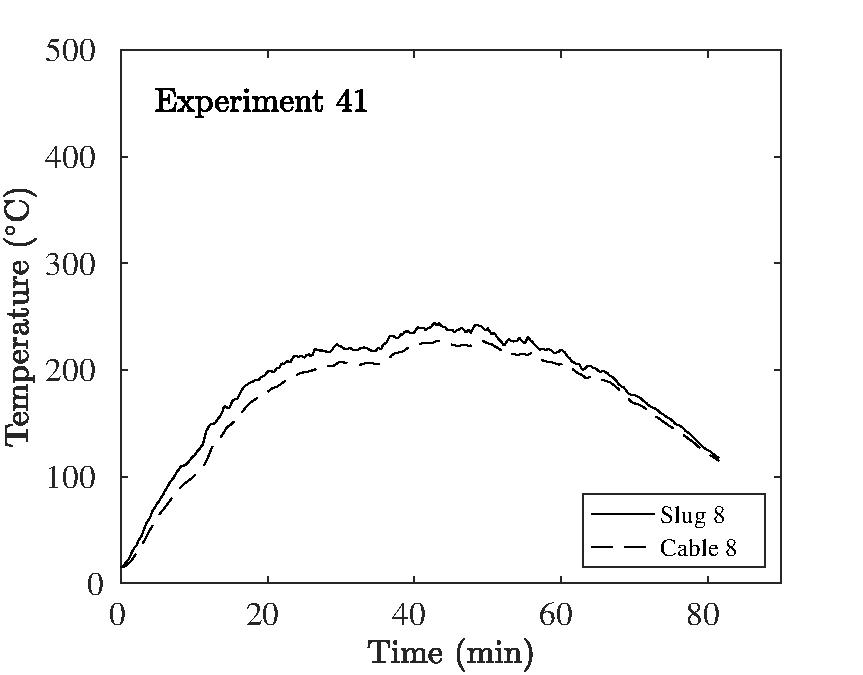
\includegraphics[height=2.2in]{../SCRIPT_FIGURES/Test_41_Plot_3} &
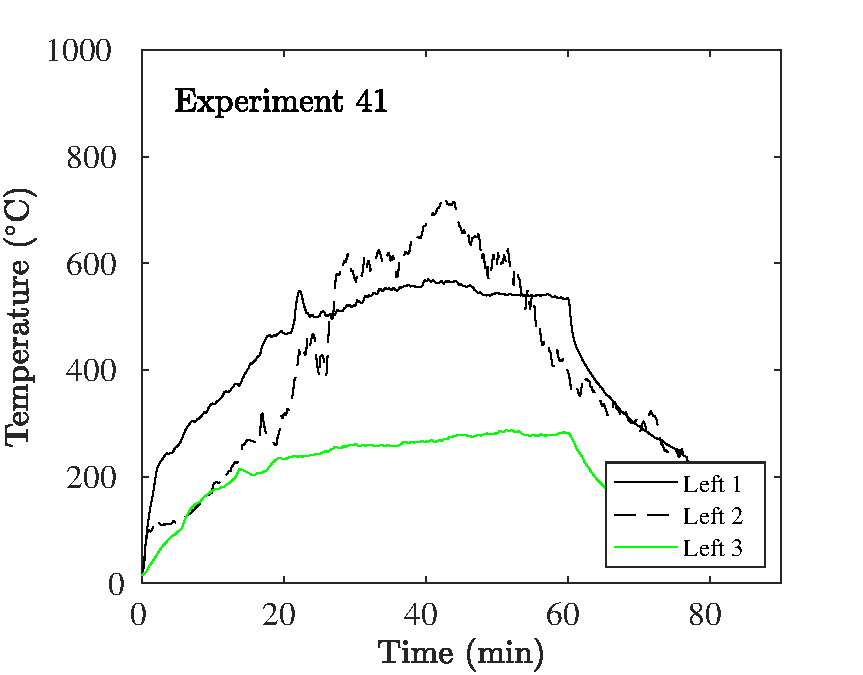
\includegraphics[height=2.2in]{../SCRIPT_FIGURES/Test_41_Plot_5}
\end{tabular*}
\caption[HRR and temperatures of Experiment 41]{The curve labeled ``Burner'' in the upper left plot represents the ideal HRR based on natural gas flow, and ``Total'' is the HRR measured via oxygen-consumption calorimetry. The curves labeled ``Slug X'' and ``Cable X'' are temperatures of cables and aluminum  rods (slugs) in the cable tray above the enclosure. All were placed above the location of the fire, but those labeled with a 7 were to the rear of the tray; 8 to the front. The gas temperatures shown in the lower right plot refer to the lower breaker compartment (``Left 3''), upper breaker (``Left 2''), and top compartment with panel wire (``Left 1'').}
\label{fig:Test_41}
\end{figure}

\begin{figure}[p]
\centering
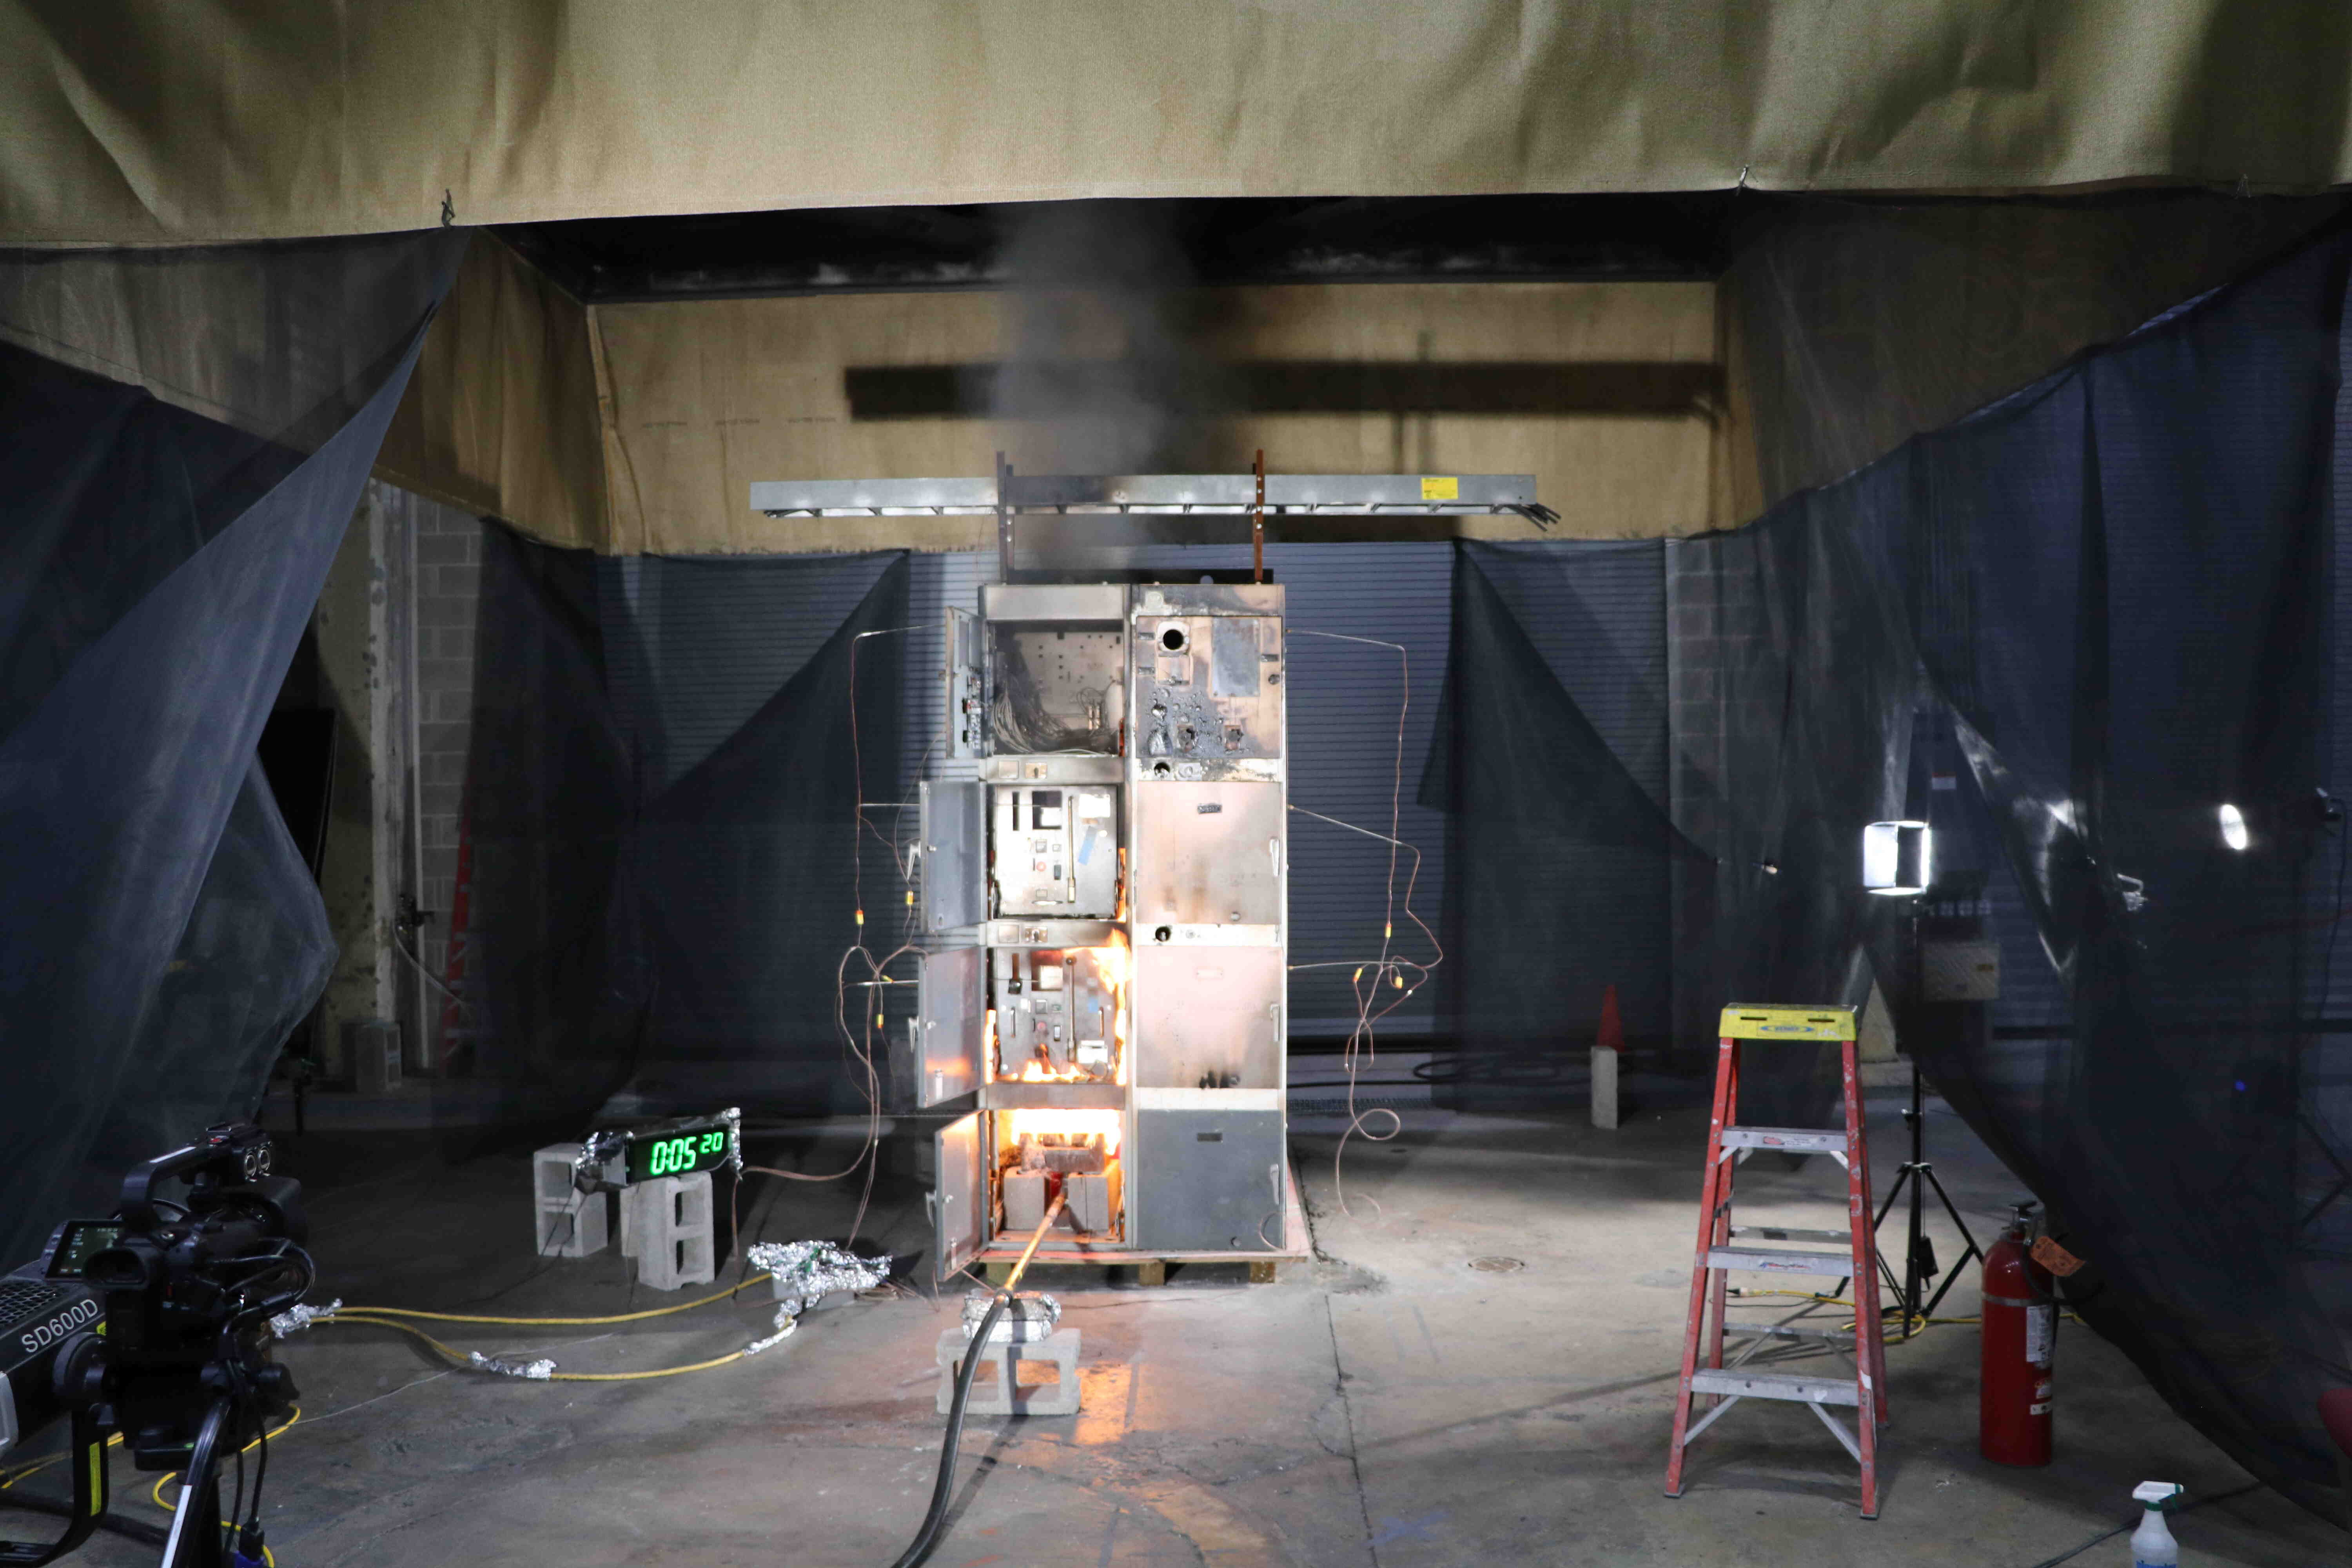
\includegraphics[height=2.50in]{../FIGURES/Test_41_5_min_20_s} \\ \vspace{0.1in}
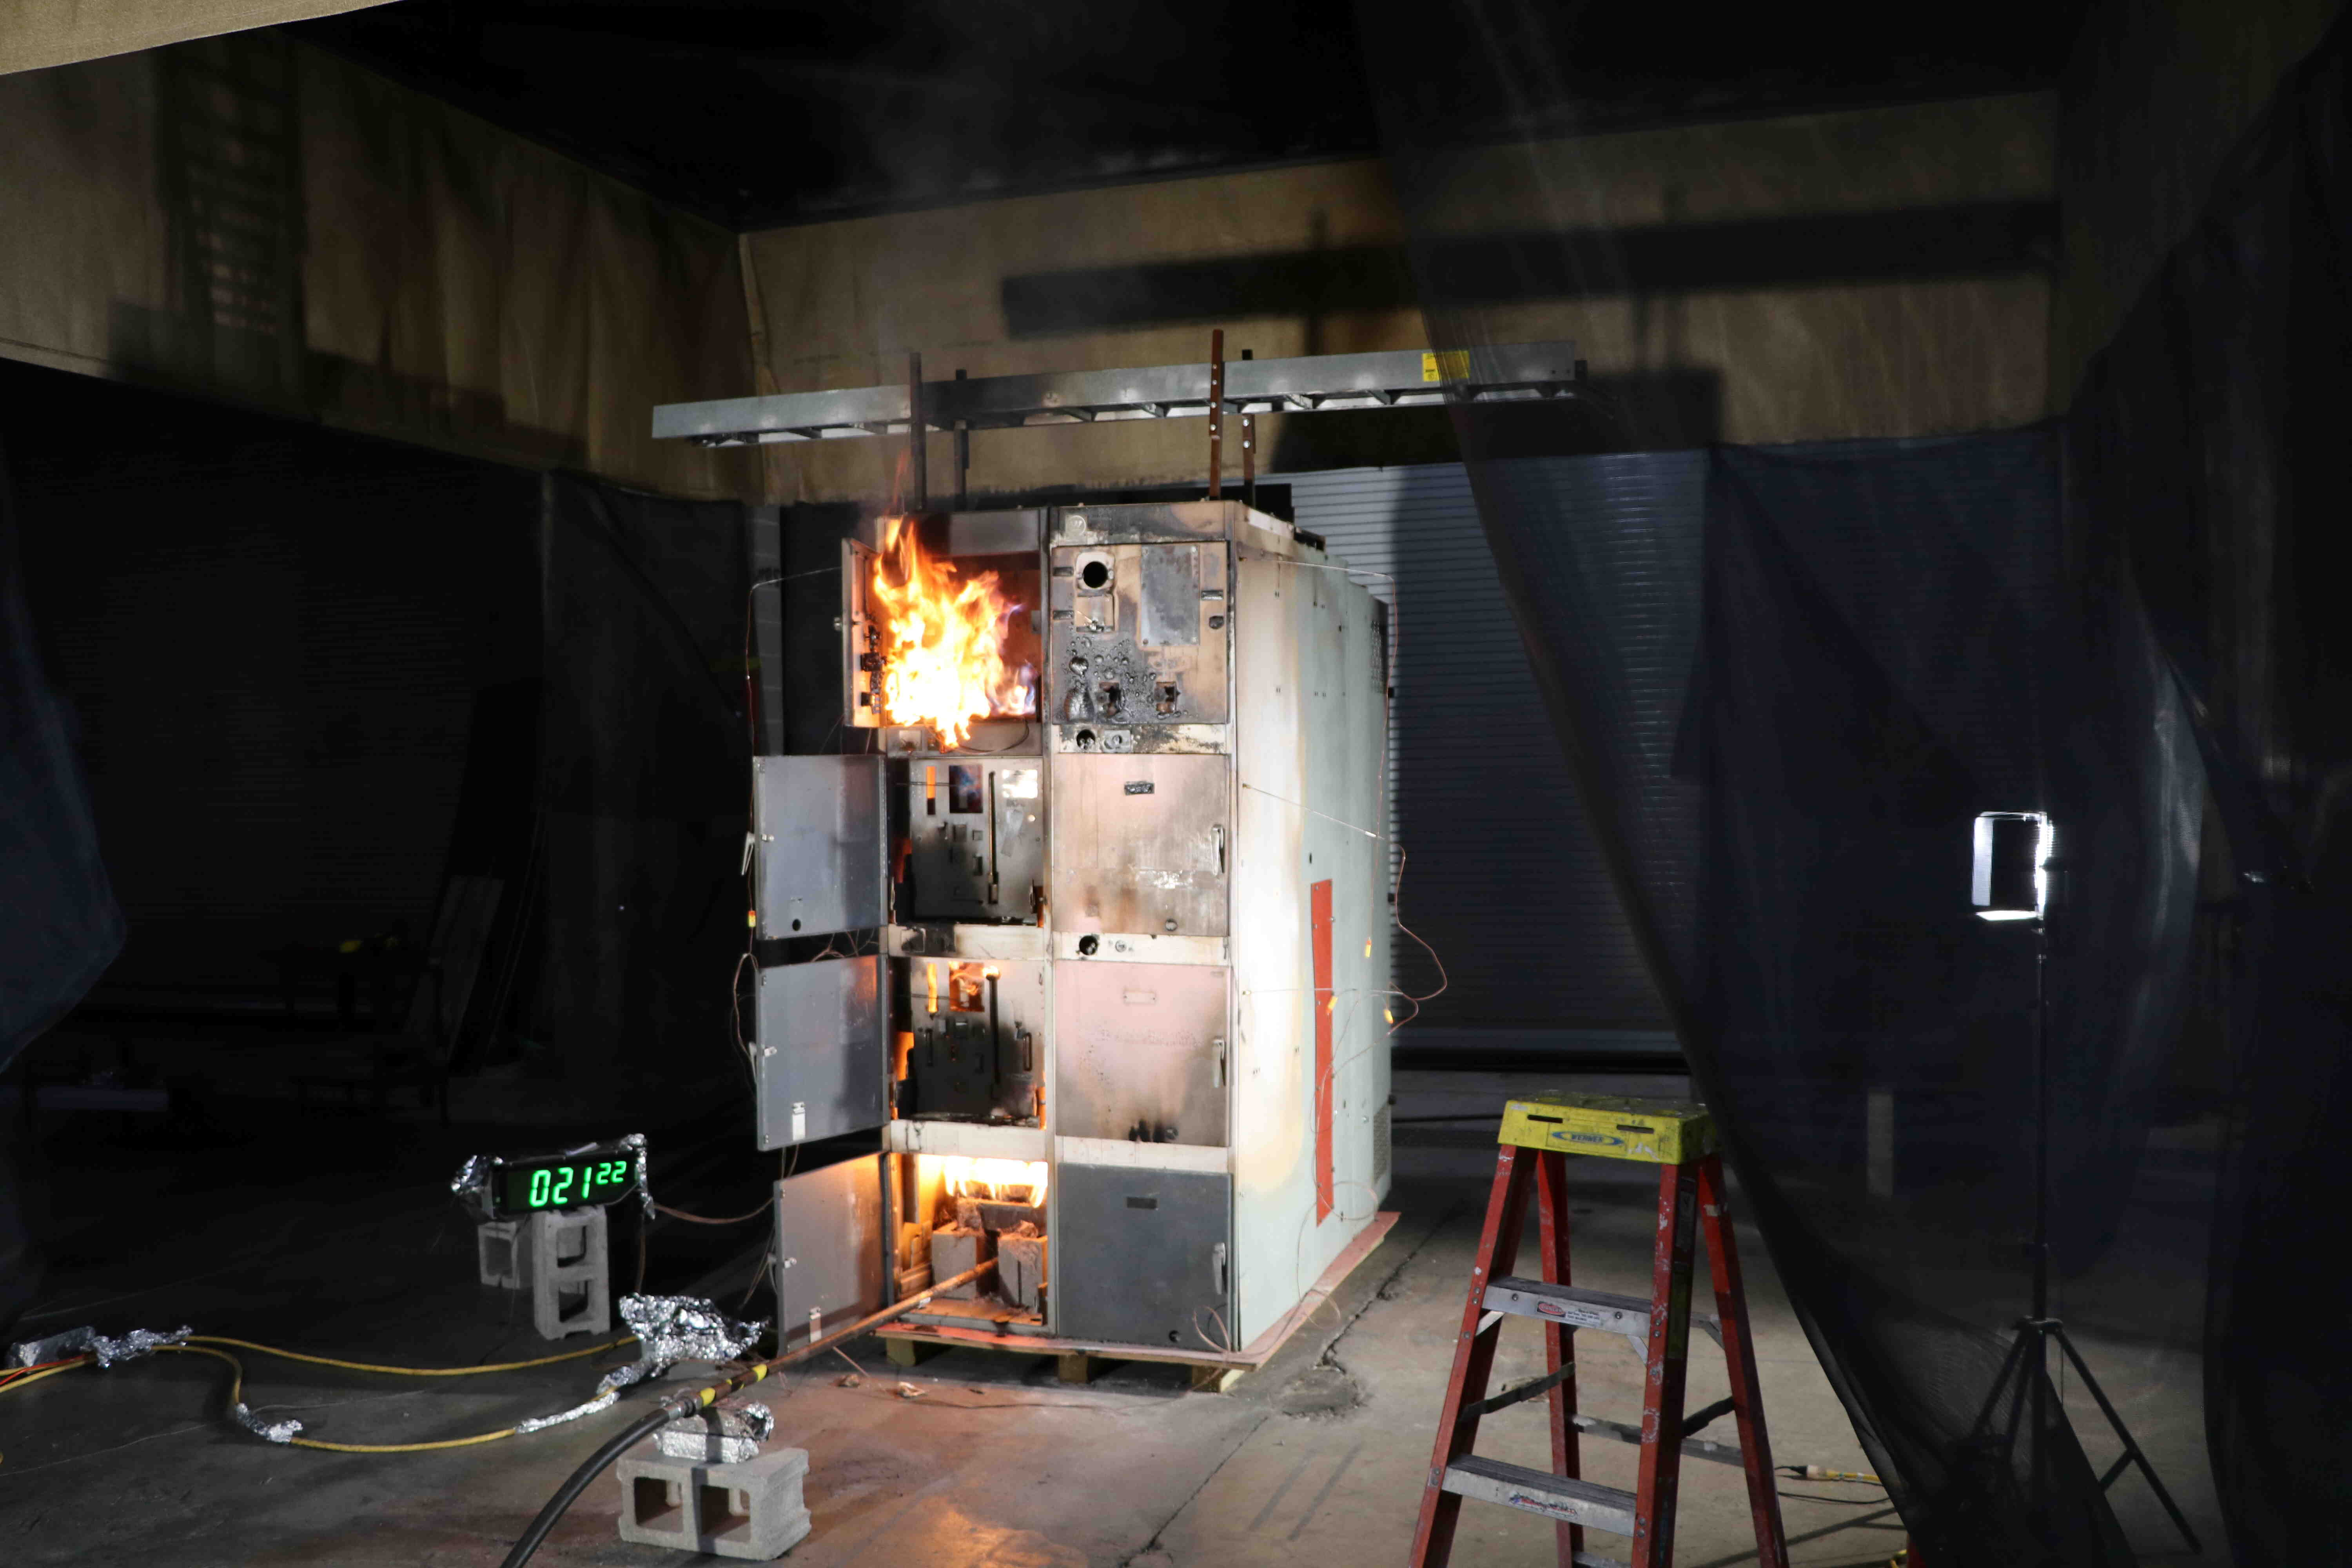
\includegraphics[height=2.50in]{../FIGURES/Test_41_21_min_22_s} \\ \vspace{0.1in}
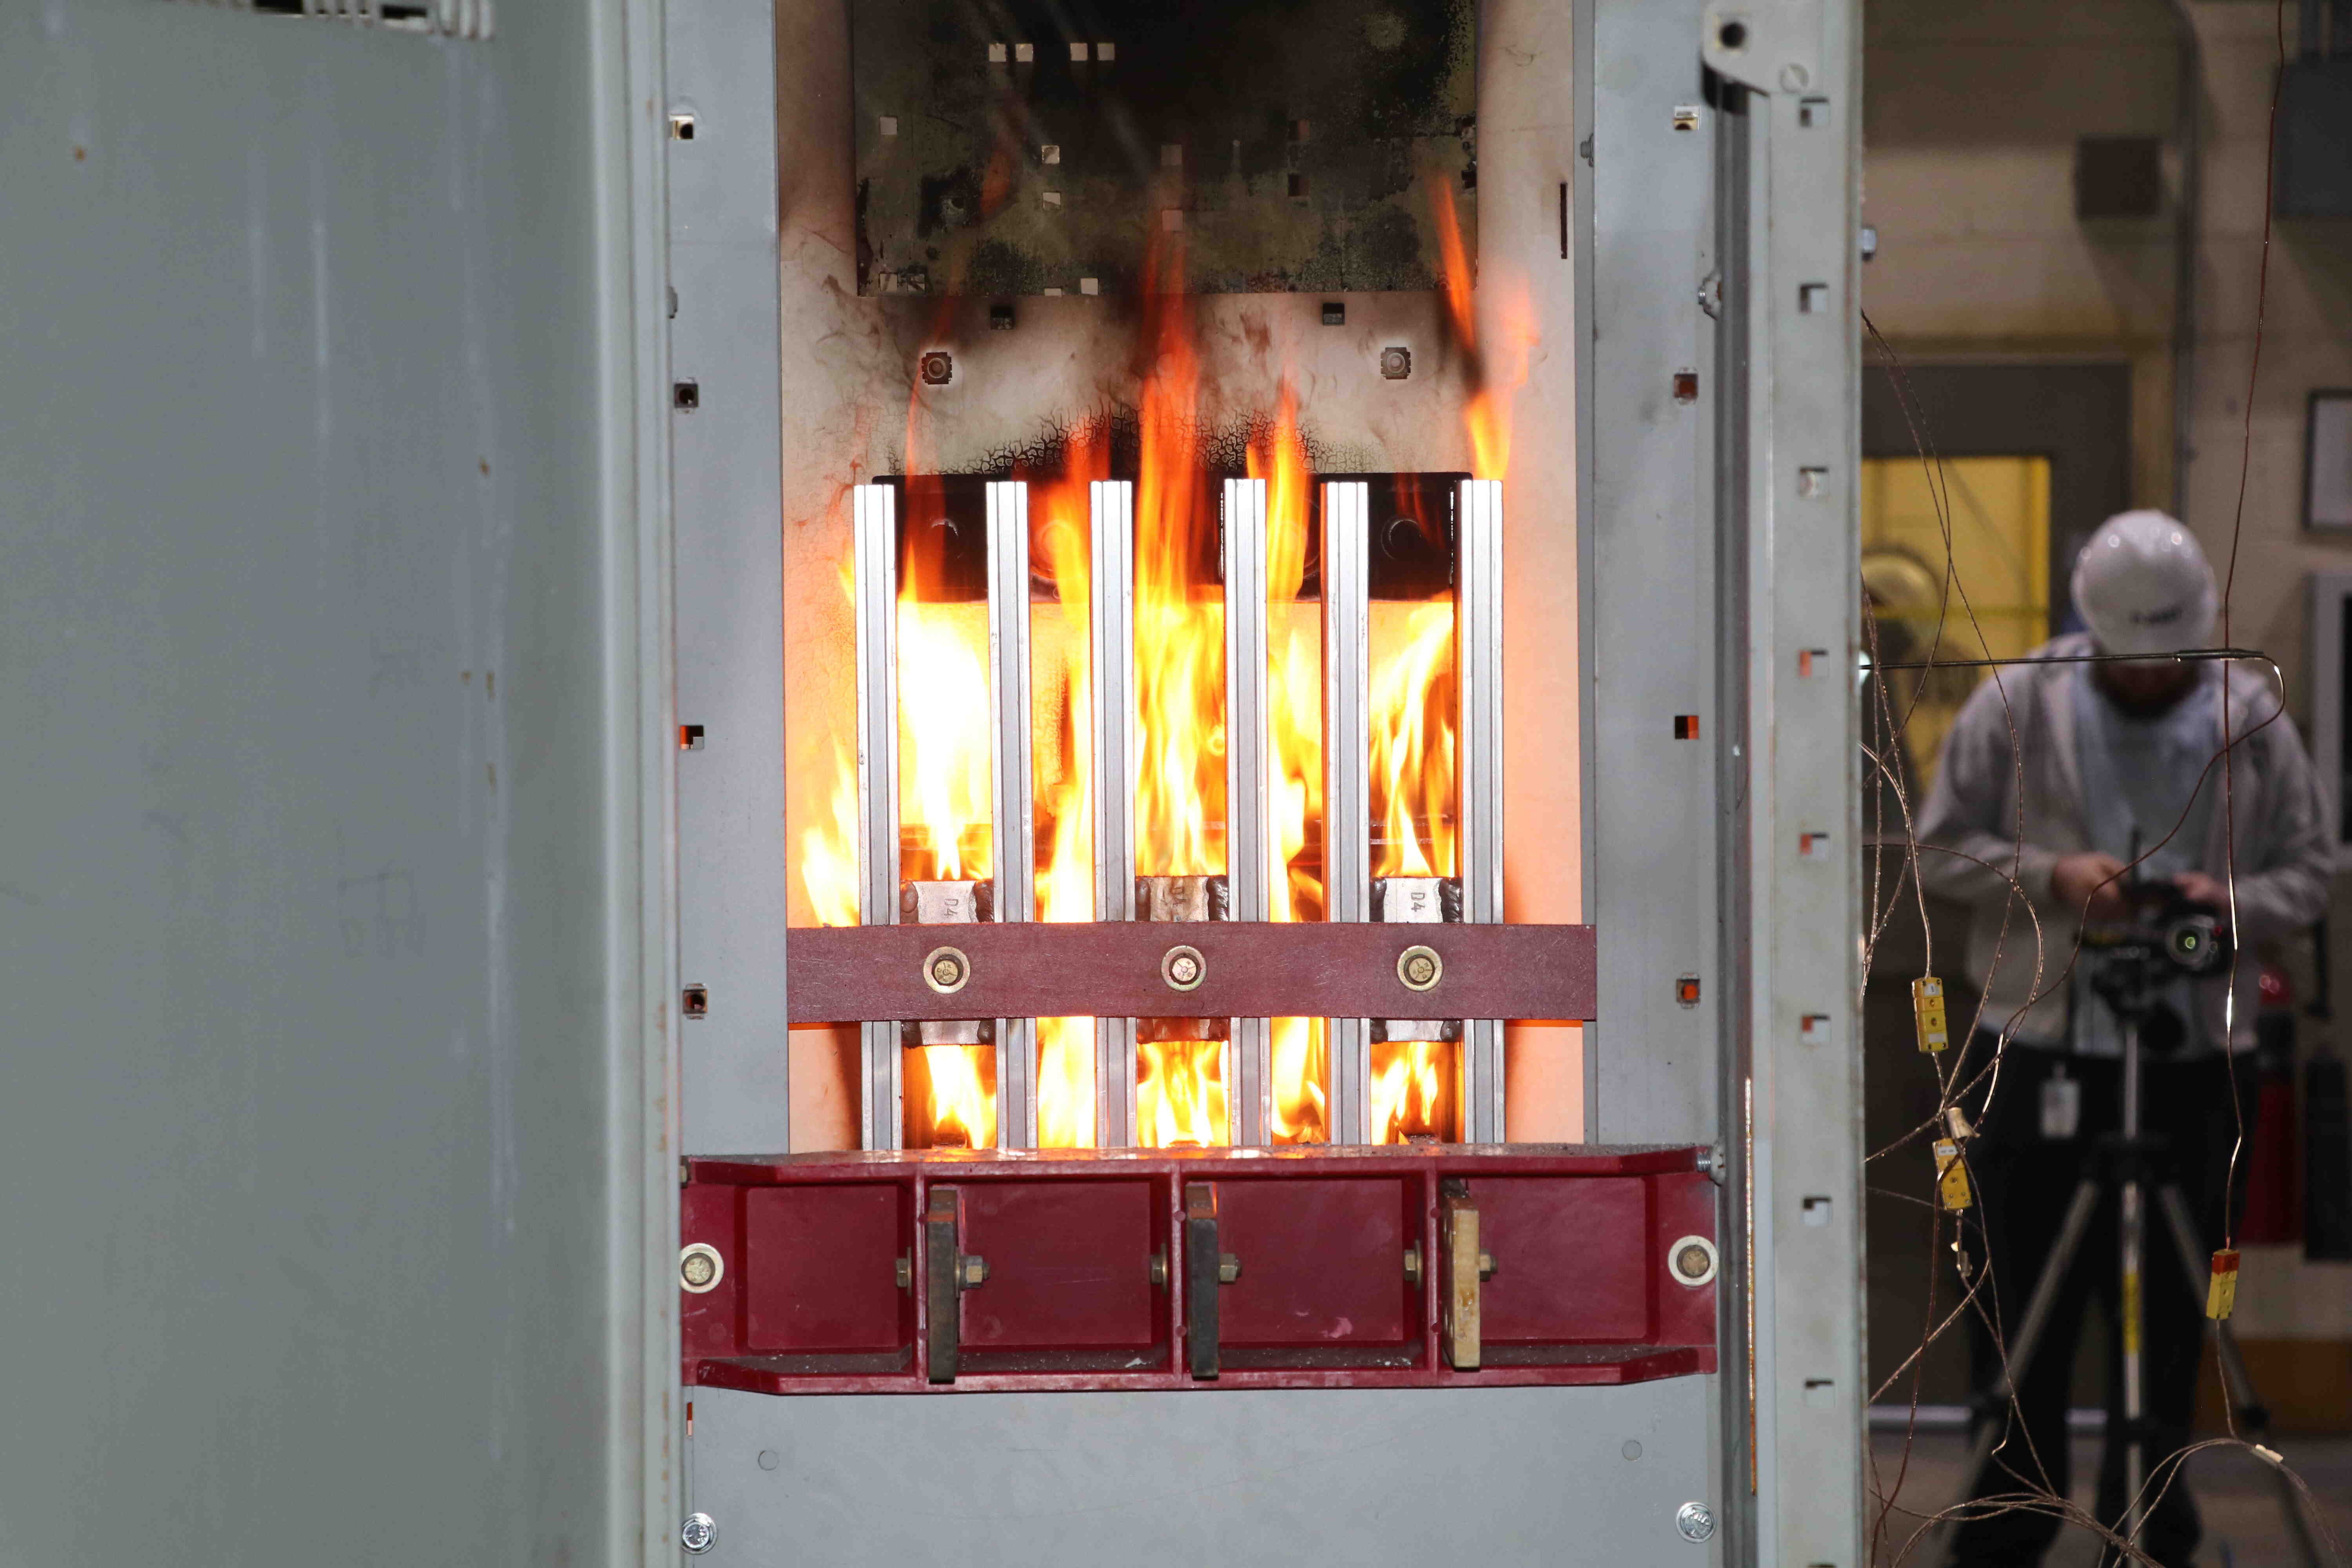
\includegraphics[height=2.50in]{../FIGURES/Test_41_rear}
\caption[Photographs of Experiment~41]{Photographs of Experiment~41. The top photograph shows the fire at 5~min, 20~s. The middle photograph shows the material burning in the uppermost compartment at 21~min, 22~s. The bottom photograph shows burning plastic insulation material at the rear of the enclosure after the fires in the front compartments had largely burnt out. }
\label{fig:Test_41_photos}
\end{figure}






\clearpage

\section{Thermal Exposure of Cables Above a Burning Electrical Enclosure}
\label{Sec:Cables}
Three types of experiments were conducted to assess the thermal exposure of electrical cables above a burning enclosure:
\begin{enumerate}
\item Single trays of cables were positioned above a gas burner.
\item Plume temperatures were measured above vents in a burning electrical enclosure.
\item Cable trays were exposed to fire plumes above burning enclosures.
\end{enumerate}
Two types of cables were used in these experiments. The one referred to as the ``thermoplastic'' cable has polyethylene insulation covering its seven 12~AWG\footnote{American Wire Gauge} copper conductors. Its jacket is approximately 1.9~mm thick polyvinyl chloride (PVC). The cable is approximately 15.9~mm (0.63~in) in diameter and has a mass of 0.38~kg/m. It is approximately 55~\% by mass copper, 27~\% jacket, 10~\% insulation, and 8~\% filler; its thermal capacity is approximately 0.36~kJ/(K~m).

The cable referred to as the ``thermoset'' has cross-linked polyethylene insulation covering its twelve 18~AWG copper conductors. Its jacket is approximately 1.5~mm thick chlorosulfonated polyethylene (CSPE). The cable is approximately 12.7~mm (0.5~in) in diameter and has a mass of 0.25~kg/m. It is approximately 37~\% by mass copper, 33~\% jacket, 29~\% insulation, and 1~\% filler; its thermal capacity is approximately 0.22~kJ/(K~m).

\subsection{Single Tray Ignition Study}

In these experiments, a single 45~cm (18~in) wide tray containing either thermoplastic or thermoset cables was positioned above a nominally 30~cm (12~in) square natural gas burner with an HRR of approximately 40~kW. Some of the cables had Type-K thermocouple embedded with an aluminum rod (``slug'') positioned alongside. The purpose of the experiments was two-fold: (1) to provide measurements of internal cable temperature and ignition time, and (2) to assess the use of the aluminum slugs as a surrogate for actual cables in testing of this sort.



\clearpage

\subsubsection{Experiment 36}

A nominally 45~cm (18~in) wide tray containing 13 thermoplastic cables was placed approximately 36~cm (14~in) above a nominally 30~cm square 40~kW natural gas burner. Thermocouples were inserted into the center of three cables above the burner, and instrumented aluminum rods (``slugs'') were placed alongside the instrumented cables. The figures below show the HRR of the gas burner and the total HRR of the burner and cables, along with the internal temperatures of the cables and slugs. The cable ignited at approximately 3~min.

\begin{figure}[!ht]
\begin{tabular*}{\textwidth}{l@{\extracolsep{\fill}}r}
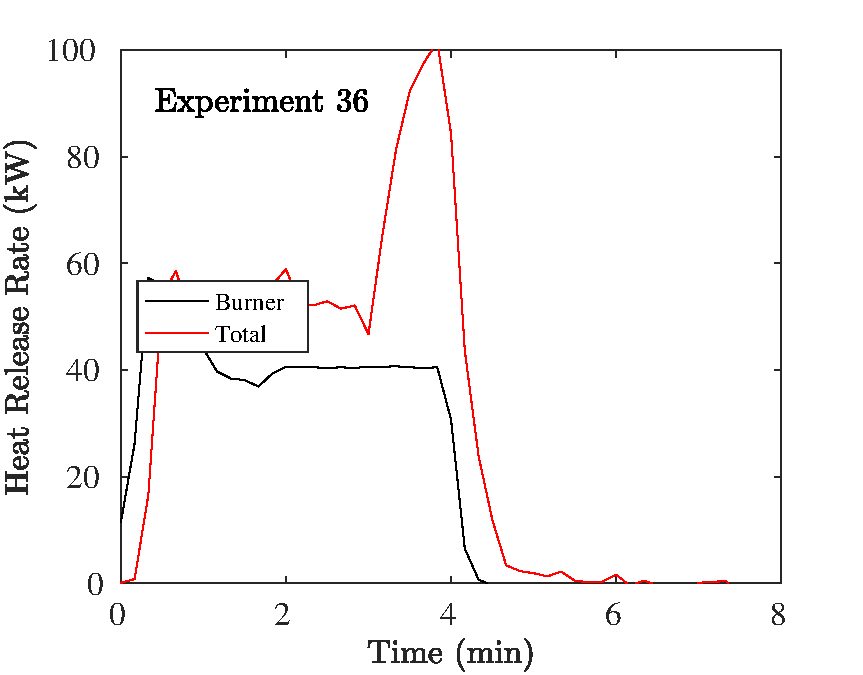
\includegraphics[height=2.40in]{../SCRIPT_FIGURES/Test_36_Plot_1} &
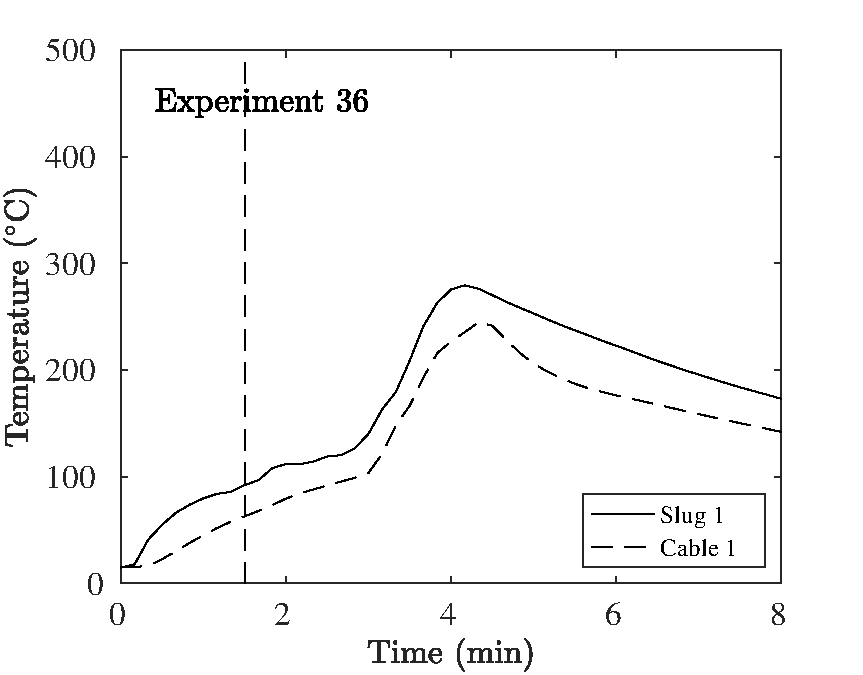
\includegraphics[height=2.40in]{../SCRIPT_FIGURES/Test_36_Plot_2} \\
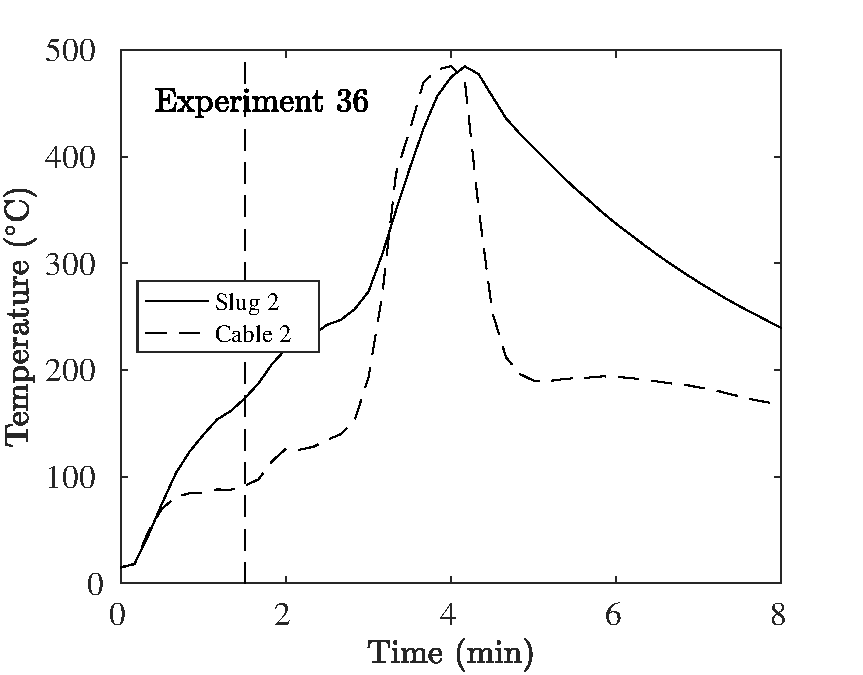
\includegraphics[height=2.40in]{../SCRIPT_FIGURES/Test_36_Plot_3} &
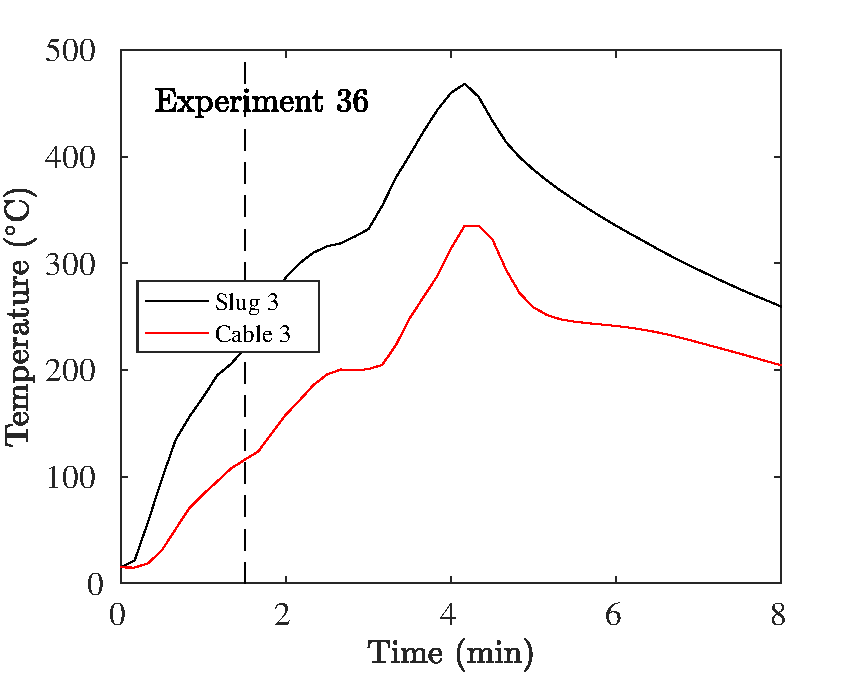
\includegraphics[height=2.40in]{../SCRIPT_FIGURES/Test_36_Plot_4}
\end{tabular*}
\caption[HRR and temperatures of Experiment 36]{Heat release rate (upper left) and internal cable and slug temperatures above a 40~kW burner. The curve labeled ``Burner'' in the upper left plot represents the ideal HRR based on natural gas flow, and ``Total'' is the HRR measured via oxygen-consumption calorimetry. The vertical dashed line indicates cable ignition.}
\label{fig:Test_36}
\end{figure}

\begin{figure}[p]
\centering
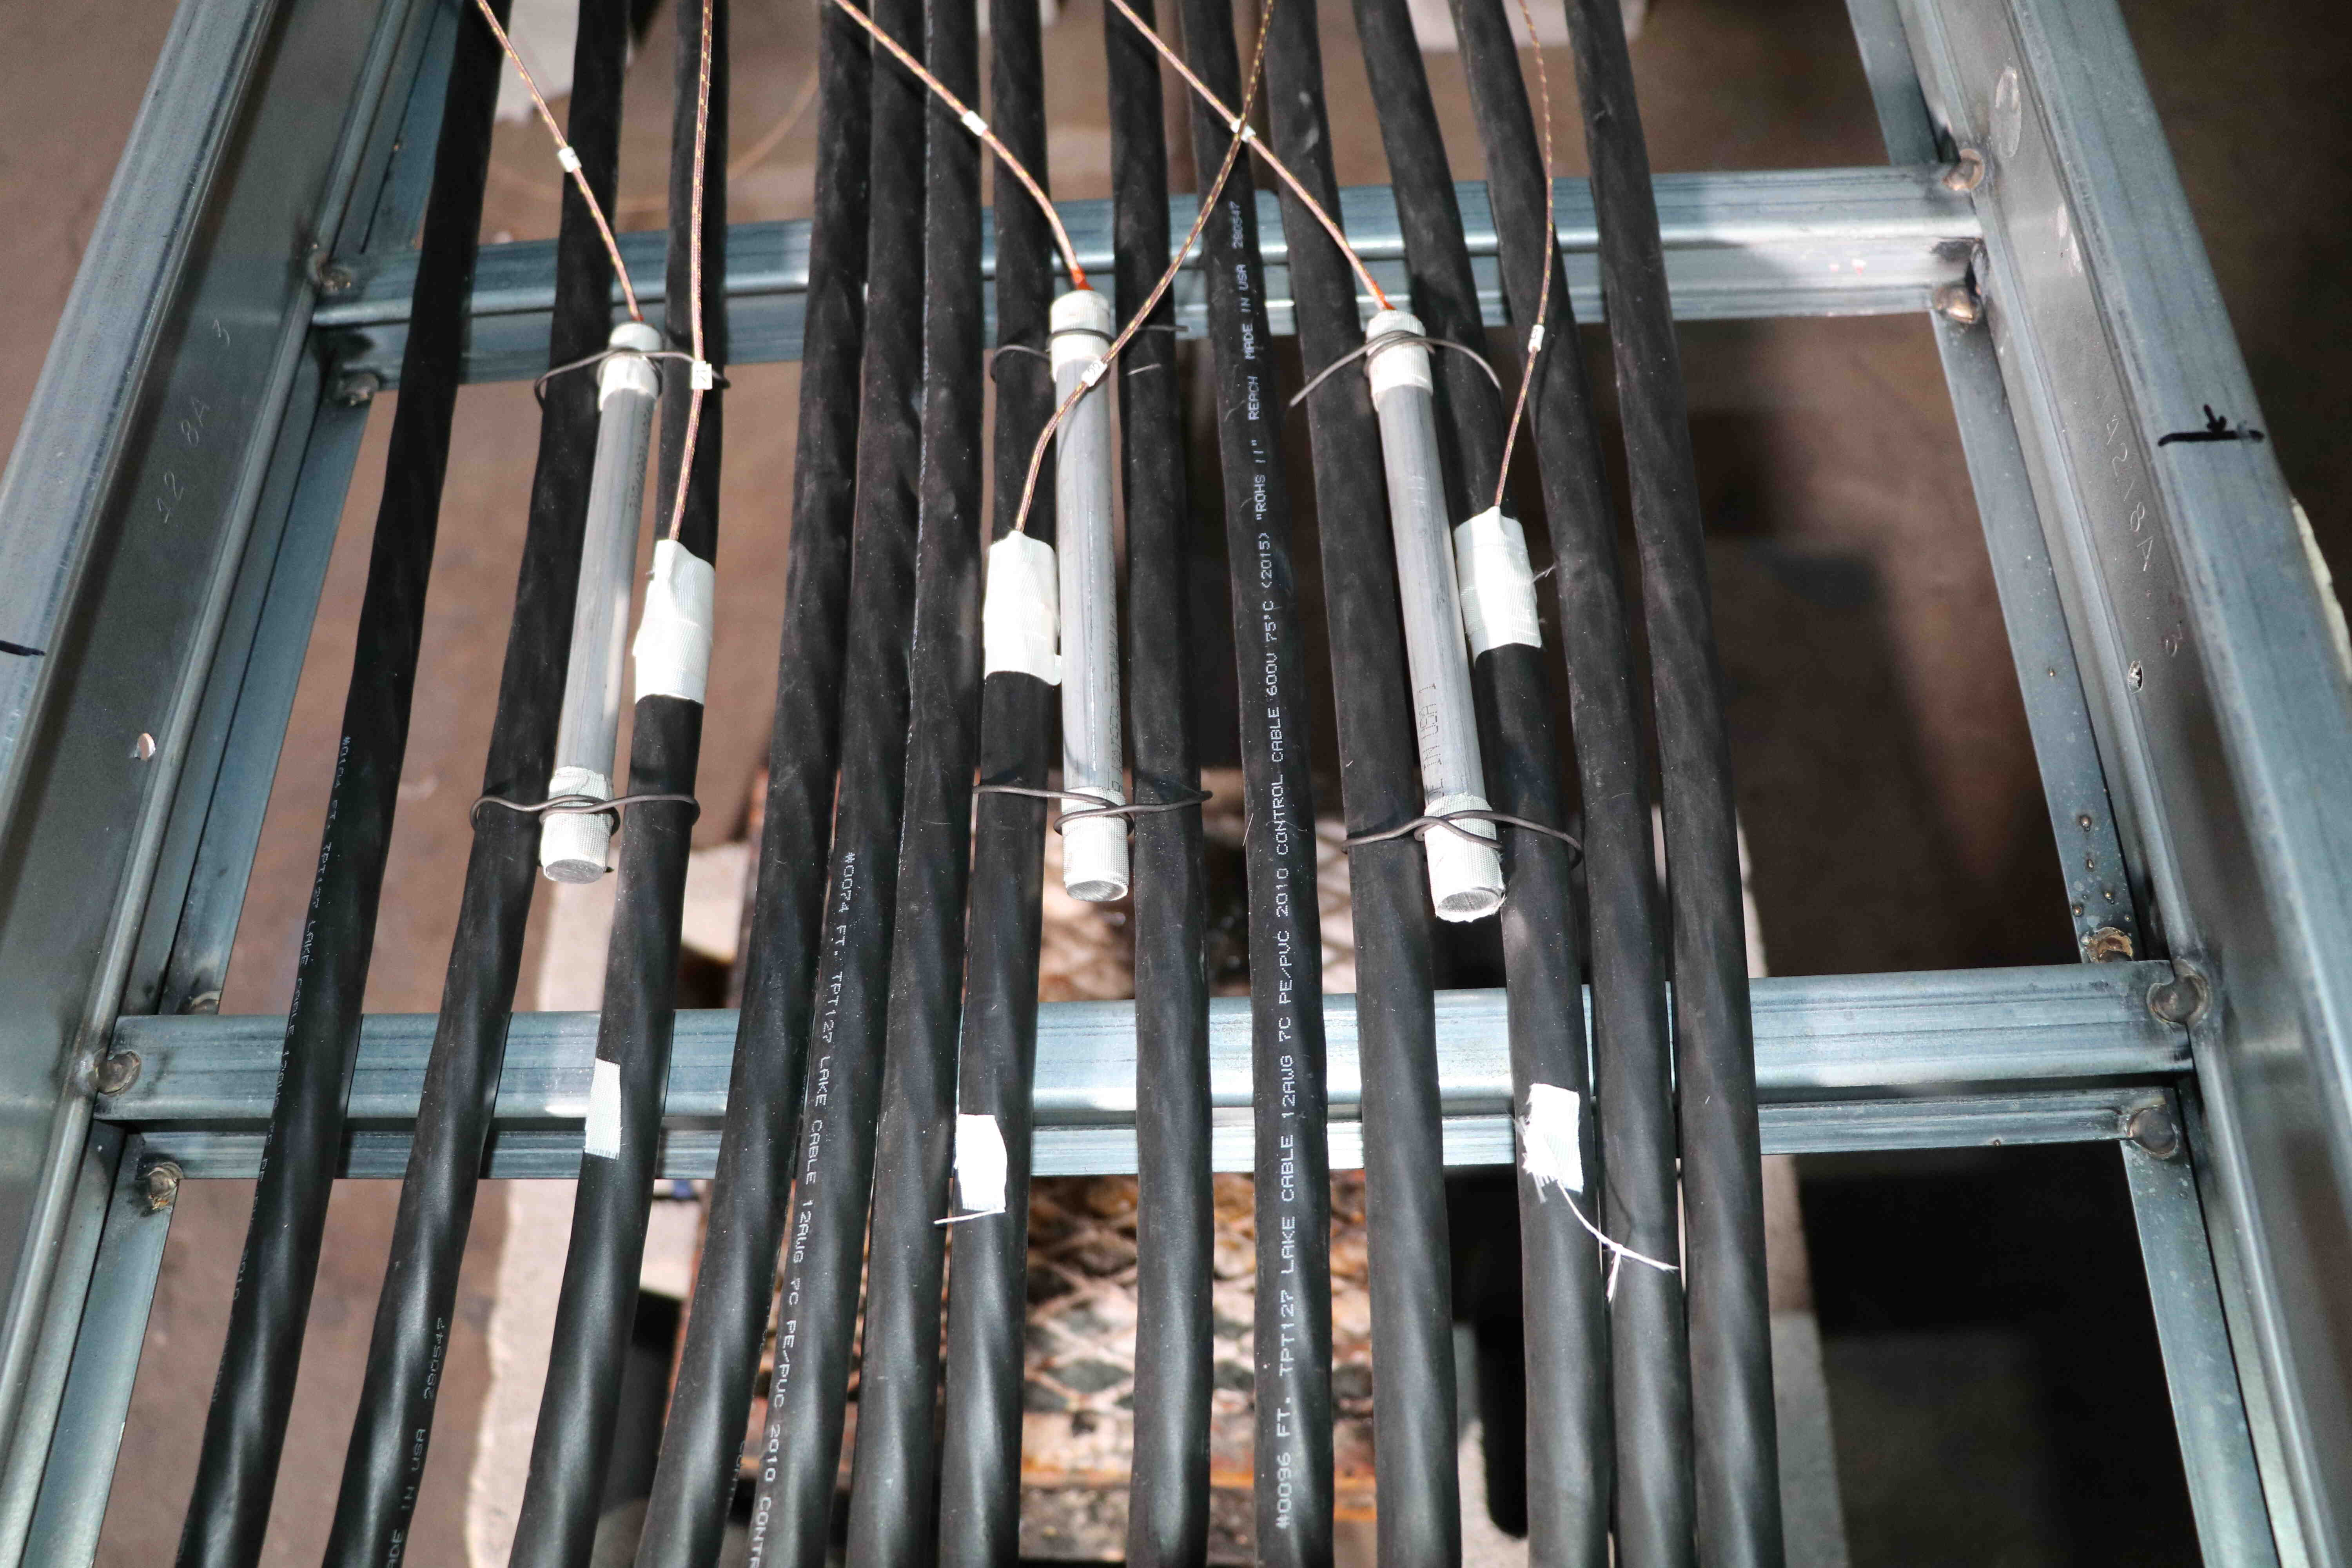
\includegraphics[height=2.50in]{../FIGURES/Test_36_setup} \\ \vspace{0.1in}
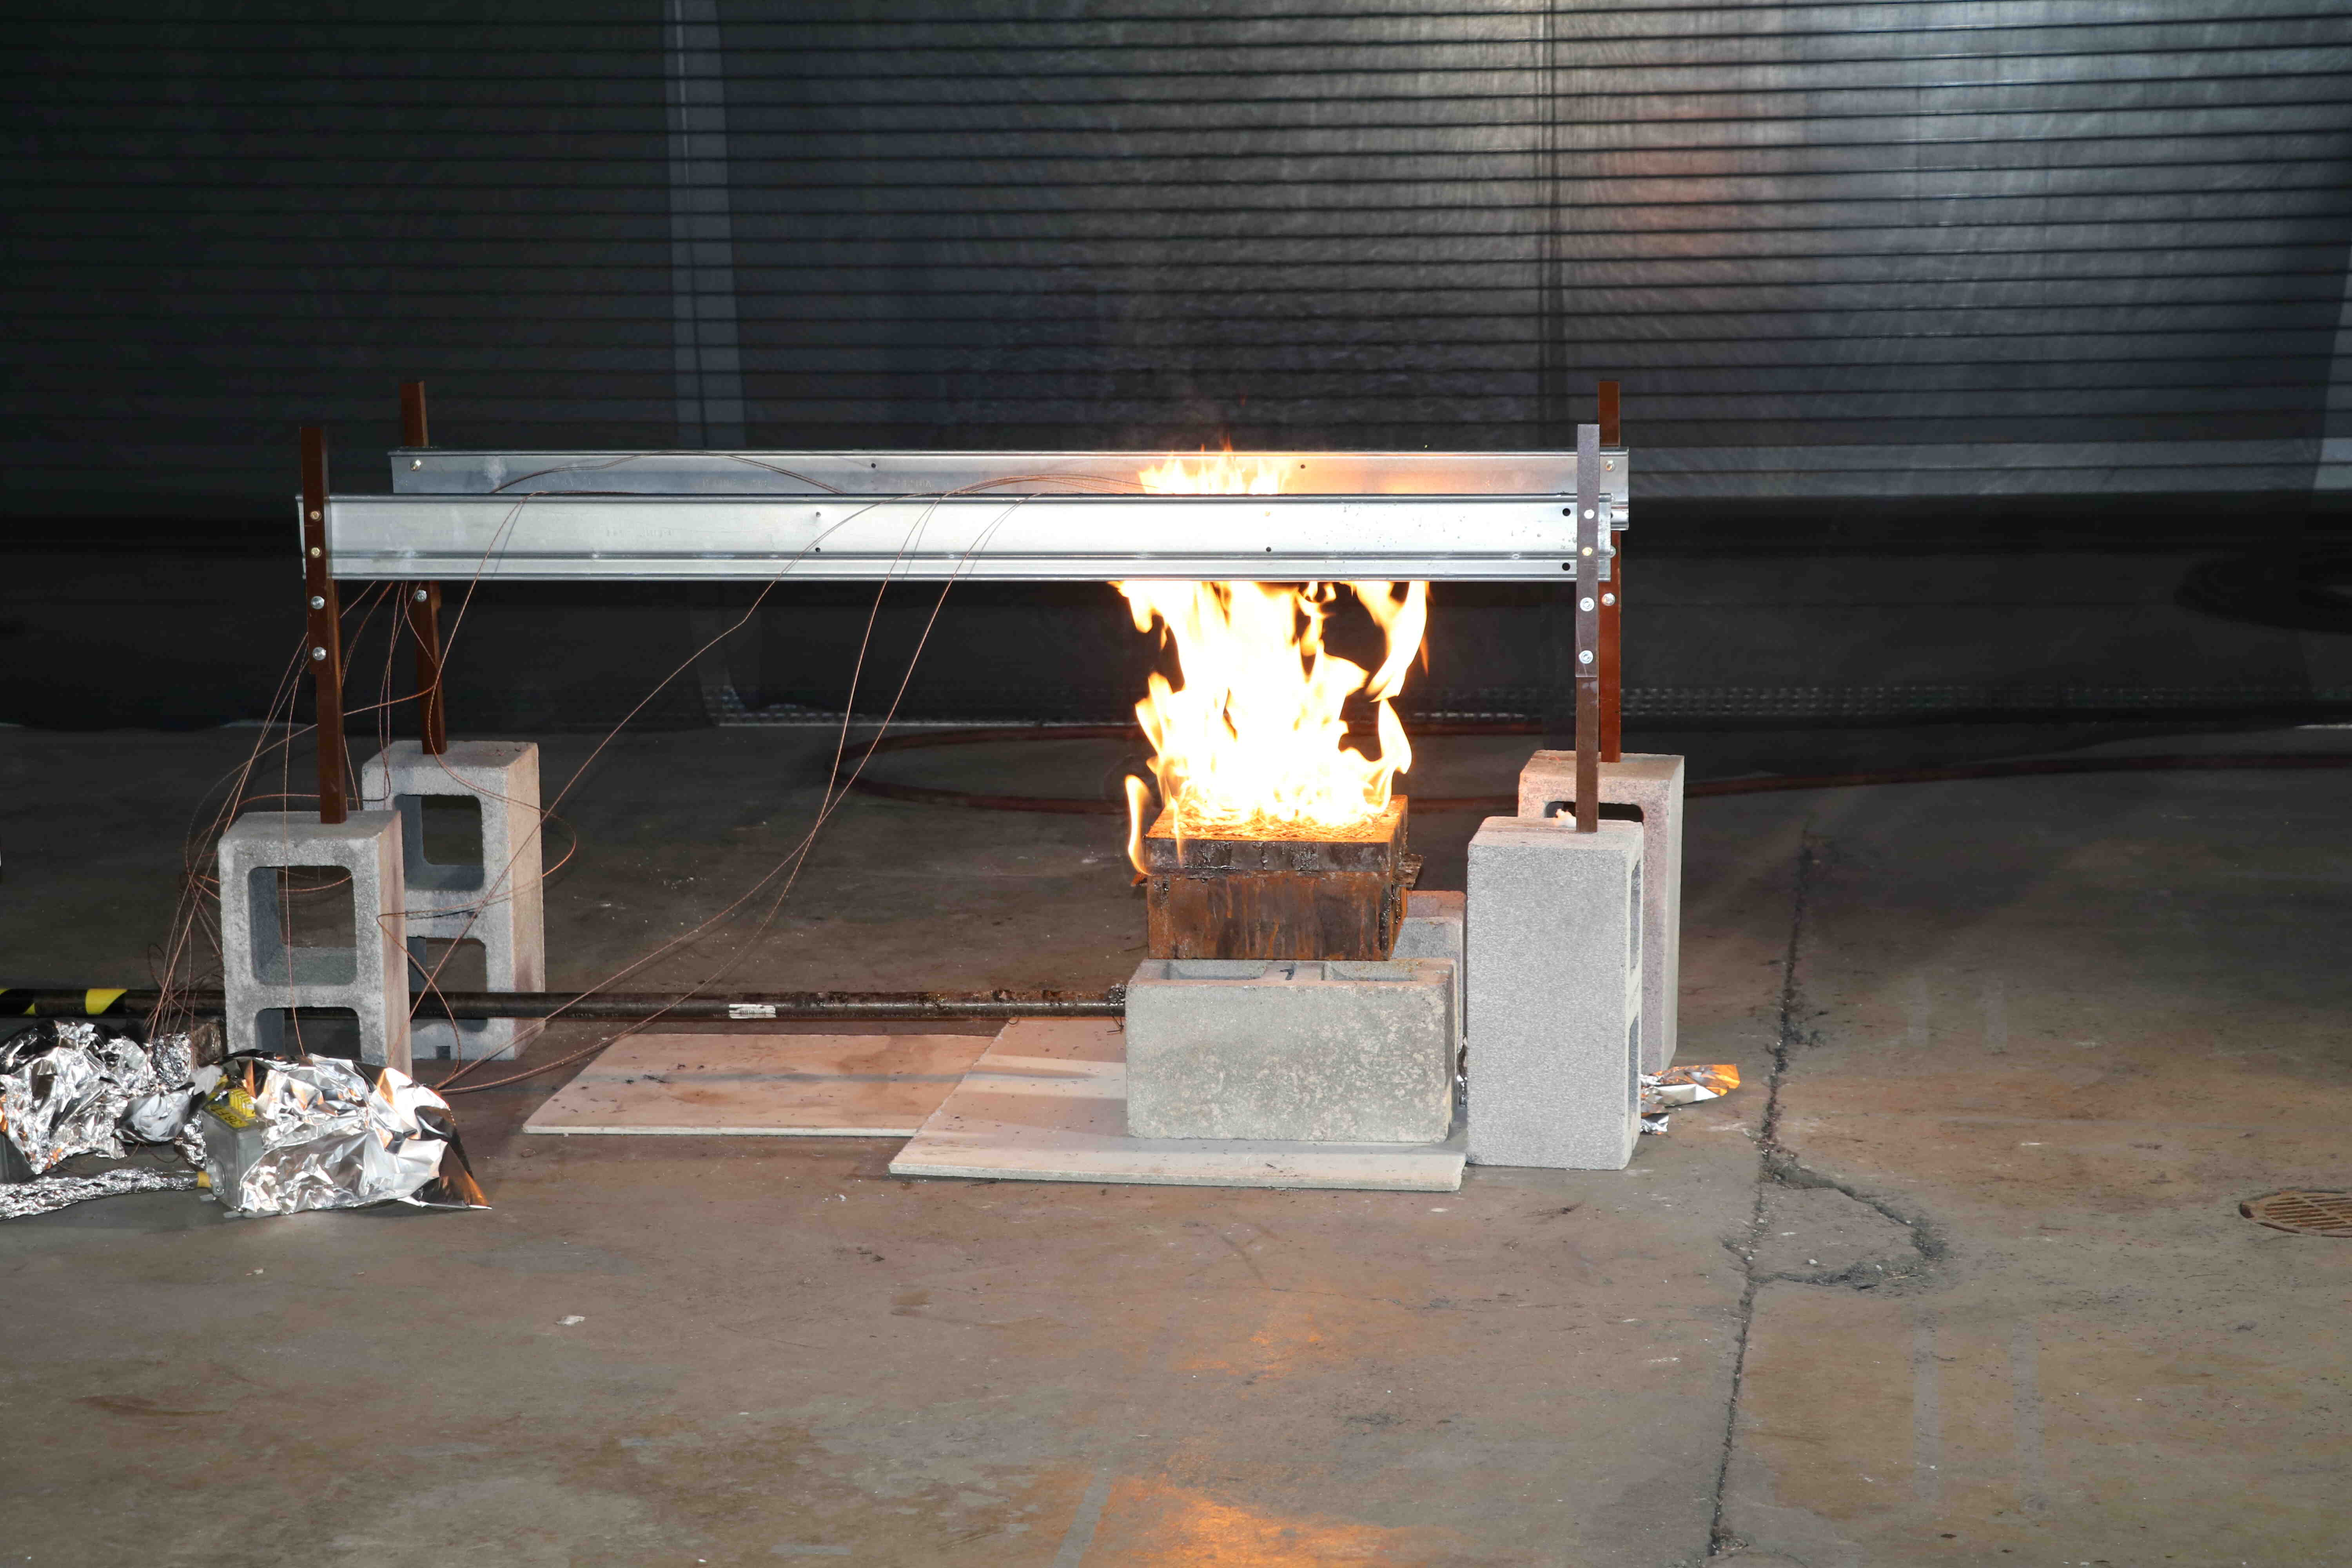
\includegraphics[height=2.50in]{../FIGURES/Test_36_side} \\ \vspace{0.1in}
\includegraphics[height=2.50in]{../FIGURES/Test_36_1_min_31_s}
\caption[Photographs of Experiment~36]{Photographs of Experiment~36. The opt photograph shows the arrangement of cables and instrumentation. The middle photograph shows the fire just at the point of cable ignition. The bottom photograph shows the burning cables at approximately the same time.}
\label{fig:Test_36_photos}
\end{figure}


\clearpage

\subsubsection{Experiment 37}

A nominally 45~cm (18~in) wide tray containing 13 thermoplastic cables was placed approximately 56~cm (22~in) above a nominally 30~cm square 40~kW natural gas burner. Thermocouples were inserted into three cables above the burner, and instrumented aluminum rods (``slugs'') were placed alongside the instrumented cables. The figures below show the HRR of the gas burner and the total HRR of the burner and cables, along with the internal temperatures of the cables and slugs. The cables ignited at approximately 4~min.

\begin{figure}[!ht]
\begin{tabular*}{\textwidth}{l@{\extracolsep{\fill}}r}
\includegraphics[height=2.40in]{../SCRIPT_FIGURES/Test_37_Plot_1} &
\includegraphics[height=2.40in]{../SCRIPT_FIGURES/Test_37_Plot_2} \\
\includegraphics[height=2.40in]{../SCRIPT_FIGURES/Test_37_Plot_3} &
\includegraphics[height=2.40in]{../SCRIPT_FIGURES/Test_37_Plot_4}
\end{tabular*}
\caption[HRR and temperatures of Experiment 37]{Heat release rate (upper left) and internal cable and slug temperatures above a 40~kW burner. The curve labeled ``Burner'' in the upper left plot represents the ideal HRR based on natural gas flow, and ``Total'' is the HRR measured via oxygen-consumption calorimetry. The vertical dashed line indicates cable ignition.}
\label{fig:Test_37}
\end{figure}

\begin{figure}[p]
\centering
\includegraphics[height=2.50in]{../FIGURES/Test_37_side} \\ \vspace{0.1in}
\includegraphics[height=2.50in]{../FIGURES/Test_37_1_min_36_s} \\ \vspace{0.1in}
\includegraphics[height=2.50in]{../FIGURES/Test_37_ignition}
\caption[Photographs of Experiment~37]{Photographs of Experiment~37. The top photograph shows the fire 14~s after the burner was ignited. The middle photograph shows the fire at 1~min, 36~s. The bottom photograph shows the cables igniting at approximately 4~min.}
\label{fig:Test_37_photos}
\end{figure}


\clearpage

\subsubsection{Experiment 38}

A nominally 45~cm (18~in) wide tray containing 12 thermoset cables was placed approximately 56~cm (22~in) above a nominally 30~cm square 40~kW natural gas burner. Thermocouples were inserted into three cables above the burner, and instrumented aluminum rods (``slugs'') were placed alongside the instrumented cables. The figures below show the HRR of the gas burner and the total HRR of the burner and cables, along with the internal temperatures of the cables and slugs. The cables did not ignite.

\begin{figure}[!ht]
\begin{tabular*}{\textwidth}{l@{\extracolsep{\fill}}r}
\includegraphics[height=2.40in]{../SCRIPT_FIGURES/Test_38_Plot_1} &
\includegraphics[height=2.40in]{../SCRIPT_FIGURES/Test_38_Plot_2} \\
\includegraphics[height=2.40in]{../SCRIPT_FIGURES/Test_38_Plot_3} &
\includegraphics[height=2.40in]{../SCRIPT_FIGURES/Test_38_Plot_4}
\end{tabular*}
\caption[HRR and temperatures of Experiment 38]{Heat release rate (upper left) and internal cable and slug temperatures above a 40~kW burner. The curve labeled ``Burner'' in the upper left plot represents the ideal HRR based on natural gas flow, and ``Total'' is the HRR measured via oxygen-consumption calorimetry.}
\label{fig:Test_38}
\end{figure}

\begin{figure}[p]
\centering
\includegraphics[height=2.50in]{../FIGURES/Test_38_setup} \\ \vspace{0.1in}
\includegraphics[height=2.50in]{../FIGURES/Test_38_29_min_29_s} \\ \vspace{0.1in}
\includegraphics[height=2.50in]{../FIGURES/Test_38_damage}
\caption[Photographs of Experiment~38]{Photographs of Experiment~38. The top photograph shows the cable trays elevated an extra 20~cm (8~in) on cement blocks. The middle photograph shows the fire at 29~min, 29~s. The bottom photograph shows the scorched cable jackets. The cables did not ignite.}
\label{fig:Test_38_photos}
\end{figure}


\clearpage

\subsubsection{Experiment 39}

A nominally 45~cm (18~in) wide tray containing 12 thermoset cables was placed approximately 36~cm (14~in) above a nominally 30~cm square 40~kW natural gas burner. Thermocouples were inserted into three cables above the burner, and instrumented aluminum rods (``slugs'') were placed alongside the instrumented cables. The figures below show the HRR of the gas burner and the total HRR of the burner and cables, along with the internal temperatures of the cables and slugs. The cables ignited at approximately 1~min, 10~s.

\begin{figure}[!ht]
\begin{tabular*}{\textwidth}{l@{\extracolsep{\fill}}r}
\includegraphics[height=2.40in]{../SCRIPT_FIGURES/Test_39_Plot_1} &
\includegraphics[height=2.40in]{../SCRIPT_FIGURES/Test_39_Plot_2} \\
\includegraphics[height=2.40in]{../SCRIPT_FIGURES/Test_39_Plot_3} &
\includegraphics[height=2.40in]{../SCRIPT_FIGURES/Test_39_Plot_4}
\end{tabular*}
\caption[HRR and temperatures of Experiment 39]{Heat release rate (upper left) and internal cable and slug temperatures above a 40~kW burner. The curve labeled ``Burner'' in the upper left plot represents the ideal HRR based on natural gas flow, and ``Total'' is the HRR measured via oxygen-consumption calorimetry. The vertical dashed line indicates cable ignition.}
\label{fig:Test_39}
\end{figure}

\begin{figure}[p]
\centering
\includegraphics[height=2.50in]{../FIGURES/Test_39_side} \\ \vspace{0.1in}
\includegraphics[height=2.50in]{../FIGURES/Test_39_1_min_36_s} \\ \vspace{0.1in}
\includegraphics[height=2.50in]{../FIGURES/Test_39_3_min_11_s}
\caption[Photographs of Experiment~39]{Photographs of Experiment~39. The top photograph shows the fire impinging on the cables. The middle photograph shows the burning cables just after ignition. The bottom photograph shows the cables a few minutes after ignition and just before self-extinguishing.}
\label{fig:Test_39_photos}
\end{figure}


\clearpage

\subsubsection{Experiment 45}

A nominally 45~cm (18~in) wide tray containing 34 thermoset cables was placed approximately 36~cm (14~in) above a nominally 30~cm square 40~kW natural gas burner. Thermocouples were inserted into two cables above the burner, and instrumented aluminum rods (``slugs'') were placed alongside the instrumented cables. The figures below show the HRR of the gas burner and the total HRR of the burner and cables, along with the internal temperatures of the cables and slugs. A small flame appeared in one location above the layer of cables at about 50~min, but the flame did not spread or lead to a wider, sustained ignition. Even though the cables did not fully ignite after an exposure of 1~h, but there was extensive damage and exposure of the copper wires.

\begin{figure}[!ht]
\begin{tabular*}{\textwidth}{l@{\extracolsep{\fill}}r}
\includegraphics[height=2.40in]{../SCRIPT_FIGURES/Test_45_Plot_1} &
\includegraphics[height=2.40in]{../SCRIPT_FIGURES/Test_45_Plot_2} \\
\multicolumn{2}{c}{\includegraphics[height=2.40in]{../SCRIPT_FIGURES/Test_45_Plot_3}}
\end{tabular*}
\caption[HRR and temperatures of Experiment 45]{Heat release rate (upper left) and internal cable and slug temperatures above a 40~kW burner. The curve labeled ``Burner'' in the upper left plot represents the ideal HRR based on natural gas flow, and ``Total'' is the HRR measured via oxygen-consumption calorimetry. The vertical dashed line indicates cable ignition.}
\label{fig:Test_45}
\end{figure}

\begin{figure}[p]
\centering
\includegraphics[height=2.50in]{../FIGURES/Test_45_setup} \\ \vspace{0.1in}
\includegraphics[height=2.50in]{../FIGURES/Test_45_42_min_46_s} \\ \vspace{0.1in}
\includegraphics[height=2.50in]{../FIGURES/Test_45_damage}
\caption[Photographs of Experiment~45]{Photographs of Experiment~45. The top photograph shows the initial cable layer and instrumentation. The middle photograph shows the fire at 42~min, 46~s. The bottom photograph shows the damaged cables.}
\label{fig:Test_45_photos}
\end{figure}


\clearpage

\subsubsection{Experiment 46}

This experiment is similar to Exp.~45 except that every seventh cable has been removed, leaving 30 rather than 34 across the width of the tray. The figures below show the HRR of the gas burner and the total HRR of the burner and cables, along with the internal temperatures of the cables and slugs. The cables ignite at approximately 12~min.

\begin{figure}[!ht]
\begin{tabular*}{\textwidth}{l@{\extracolsep{\fill}}r}
\includegraphics[height=2.40in]{../SCRIPT_FIGURES/Test_46_Plot_1} &
\includegraphics[height=2.40in]{../SCRIPT_FIGURES/Test_46_Plot_2} \\
\multicolumn{2}{c}{\includegraphics[height=2.40in]{../SCRIPT_FIGURES/Test_46_Plot_3}}
\end{tabular*}
\caption[HRR and temperatures of Experiment 46]{Heat release rate (upper left) and internal cable and slug temperatures above a 40~kW burner. The curve labeled ``Burner'' in the upper left plot represents the ideal HRR based on natural gas flow, and ``Total'' is the HRR measured via oxygen-consumption calorimetry. The vertical dashed line indicates cable ignition.}
\label{fig:Test_46}
\end{figure}

\begin{figure}[p]
\centering
\includegraphics[height=2.50in]{../FIGURES/Test_46_setup} \\ \vspace{0.1in}
\includegraphics[height=2.50in]{../FIGURES/Test_46_ignition} \\ \vspace{0.1in}
\includegraphics[height=2.50in]{../FIGURES/Test_46_burning}
\caption[Photographs of Experiment~46]{Photographs of Experiment~46. The top photograph shows the arrangement of cables and instrumentation. The middle photograph shows the cables igniting at approximately 12~min. The bottom photograph shows the cables steadily burning at 15~min, 6~s.}
\label{fig:Test_46_photos}
\end{figure}


\clearpage

\subsubsection{Experiment 47}

A nominally 45~cm (18~in) wide tray containing 30 thermoplastic cables was placed approximately 36~cm (14~in) above a nominally 30~cm square 40~kW natural gas burner. Thermocouples were inserted into two cables above the burner, and instrumented aluminum rods (``slugs'') were placed alongside the instrumented cables. The figures below show the HRR of the gas burner and the total HRR of the burner and cables, along with the internal temperatures of the cables and slugs. The cables ignited in less than 1~min.

\begin{figure}[!ht]
\begin{tabular*}{\textwidth}{l@{\extracolsep{\fill}}r}
\includegraphics[height=2.40in]{../SCRIPT_FIGURES/Test_47_Plot_1} &
\includegraphics[height=2.40in]{../SCRIPT_FIGURES/Test_47_Plot_2} \\
\multicolumn{2}{c}{\includegraphics[height=2.40in]{../SCRIPT_FIGURES/Test_47_Plot_3}}
\end{tabular*}
\caption[HRR and temperatures of Experiment 47]{Heat release rate (upper left) and internal cable and slug temperatures above a 40~kW burner. The curve labeled ``Burner'' in the upper left plot represents the ideal HRR based on natural gas flow, and ``Total'' is the HRR measured via oxygen-consumption calorimetry. The vertical dashed line indicates cable ignition.}
\label{fig:Test_47}
\end{figure}

\begin{figure}[p]
\centering
\includegraphics[height=2.50in]{../FIGURES/Test_47_setup} \\ \vspace{0.1in}
\includegraphics[height=2.50in]{../FIGURES/Test_47_ignition} \\ \vspace{0.1in}
\includegraphics[height=2.50in]{../FIGURES/Test_47_burning}
\caption[Photographs of Experiment~47]{Photographs of Experiment~47. The top photograph shows the cable and instrumentation placement. The middle photograph shows the cables burning at 1~min, 9~s, just after ignition. The bottom photograph shows the fire at 5~min, 42~s, after the burner has been extinguished. }
\label{fig:Test_47_photos}
\end{figure}


\clearpage

\subsubsection{Experiment 48}

Experiment 48 was the same as Exp.~47 except that the tray was increased to 56~cm (22~in) above the burner. The figures below show the HRR of the gas burner and the total HRR of the burner and cables, along with the internal temperatures of the cables and slugs. The cables ignited at approximately 3~min.

\begin{figure}[!ht]
\begin{tabular*}{\textwidth}{l@{\extracolsep{\fill}}r}
\includegraphics[height=2.40in]{../SCRIPT_FIGURES/Test_48_Plot_1} &
\includegraphics[height=2.40in]{../SCRIPT_FIGURES/Test_48_Plot_2} \\
\multicolumn{2}{c}{\includegraphics[height=2.40in]{../SCRIPT_FIGURES/Test_48_Plot_3}}
\end{tabular*}
\caption[HRR and temperatures of Experiment 48]{Heat release rate (upper left) and internal cable and slug temperatures above a 40~kW burner. The curve labeled ``Burner'' in the upper left plot represents the ideal HRR based on natural gas flow, and ``Total'' is the HRR measured via oxygen-consumption calorimetry. The vertical dashed line indicates cable ignition.}
\label{fig:Test_48}
\end{figure}

\begin{figure}[p]
\centering
\includegraphics[height=2.50in]{../FIGURES/Test_48_1_min_3_s} \\ \vspace{0.1in}
\includegraphics[height=2.50in]{../FIGURES/Test_48_3_min_11_s} \\ \vspace{0.1in}
\includegraphics[height=2.50in]{../FIGURES/Test_48_3_min_28_s}
\caption[Photographs of Experiment~48]{Photographs of Experiment~48. The top photograph shows the fire 1~min, 3~s after burner ignition. The middle photograph shows cable ignition just after 3~min. The bottom photograph shows steady burning at 3~min, 28~s.}
\label{fig:Test_48_photos}
\end{figure}


\clearpage

\subsubsection{Summary}

\begin{table}[ht]
\begin{center}
\caption[Results of cable tray ignition experiments]{Ignition time of cables set above a 40~kW natural gas burner.}
\label{matrix2}
\begin{tabular}{|c|c|c|c|c|}
\hline
Exp.   &          & Cable             & Cable         & Ignition         \\
No.    & Make     & Packing           & Height        & Time             \\
       &          &                   & (cm)          & (min:s)          \\ \hline
36     & TP       & Loose             & 36            & 1:30             \\ \hline
37     & TP       & Loose             & 56            & 4:00             \\ \hline
38     & TS       & Loose             & 56            & ---              \\ \hline
39     & TS       & Loose             & 36            & 1:30             \\ \hline
45     & TS       & Tight             & 36            & 50:00            \\ \hline
46     & TS       & Tight             & 36            & 12:00            \\ \hline
47     & TP       & Tight             & 36            & 1:00             \\ \hline
48     & TP       & Tight             & 56            & 3:00             \\ \hline

\end{tabular}
\end{center}
\end{table}



\clearpage

\subsection{Measuring the Gas Temperature above a Burning Enclosure}

Following the HRR measurements in Experiments 40 and 41, the same Westinghouse enclosure was used in experiments aimed at measuring the fire plume temperature outside of a near-ceiling vertical vent. These were difficult measurements to perform because it is difficult to predict the trajectory of the plume centerline. Nevertheless, it can be seen in Experiments~42 through 45 that temperatures above a vertical vent can reach values of 400~$^\circ$C to 500~$^\circ$C (750~$^\circ$F to 930~$^\circ$F), high enough to ignite cables given enough time, a subject which is the focus of Experiments~49 through 64.



\clearpage


\subsubsection{Experiment 42}

A nominally 30~cm (12~in) square natural gas burner was positioned in the mostly empty space at the rear of the breaker enclosure used in Experiments~40 and 41. The HRR of the burner was ramped up to 200~kW following an approximate t-squared profile. Six sheathed thermocouples were positioned above the upper rear vent in an attempt to measure the plume temperature. The plume did not follow the expected pattern and the tips of the thermocouples were not exposed to the peak temperatures within the plume. Thus, this experiment is of marginal value for assessing the threat to overhead targets.

The figures below show the HRR of the gas burner, along with the temperatures measured by the sheathed thermocouples above the enclosure.

\begin{figure}[!ht]
\begin{tabular*}{\textwidth}{l@{\extracolsep{\fill}}r}
\includegraphics[height=2.40in]{../SCRIPT_FIGURES/Test_42_Plot_1} &
\includegraphics[height=2.40in]{../SCRIPT_FIGURES/Test_42_Plot_2}
\end{tabular*}
\caption[HRR and temperatures of Experiment 42]{Heat release rate (left) and sheathed thermocouple temperatures (right) above a burning breaker enclosure. The HRR measurement is based on natural gas consumption (``Burner'') and oxygen-consumption calorimetry (``Total'').}
\label{fig:Test_42}
\end{figure}

\begin{figure}[p]
\centering
\includegraphics[height=2.50in]{../FIGURES/Test_42_start} \\ \vspace{0.1in}
\includegraphics[height=2.50in]{../FIGURES/Test_42_rear} \\ \vspace{0.1in}
\includegraphics[height=2.50in]{../FIGURES/Test_42_side}
\caption[Photographs of Experiment~42]{Photographs of Experiment~42. The burner is on the right side of the enclosure and the photographs show the fire at approximately 50~kW (top), 100~kW (middle), and 200~kW (bottom). A vertical array of sheathed thermocouples sits at the upper edge of the enclosure. The cable tray in the background was left over from a previous experiment and played no role in this experiment. }
\label{fig:Test_42_photos}
\end{figure}


\clearpage

\subsubsection{Experiment 43}

A nominally 30~cm (12~in) square natural gas burner was positioned in the mostly empty space at the rear of the breaker enclosure used in Experiments~40 and 41. The HRR of the burner was ramped up to 300~kW following an approximate t-squared profile. Six aluminum rods (``slugs'') and six sheathed thermocouples were positioned above the upper rear vent in an attempt to measure the plume temperature. Two of each instrument were positioned approximately 15~cm (6~in), 30~cm (12~in), and 60~cm (24~in) above the top of the enclosure, roughly flush with the rear door.

The figures below show the HRR of the gas burner and the total HRR of the burner, along with the temperatures measured by the sheathed thermocouples and aluminum rods above the enclosure. Note that the rod temperatures show less temporal variation because of increased thermal mass. These temperatures are a better indicator of those of actual cables that might be located in the vicinity.

\begin{figure}[!ht]
\begin{tabular*}{\textwidth}{l@{\extracolsep{\fill}}r}
\includegraphics[height=2.2in]{../SCRIPT_FIGURES/Test_43_Plot_1} &
\includegraphics[height=2.2in]{../SCRIPT_FIGURES/Test_43_Plot_2} \\
\multicolumn{2}{c}{\includegraphics[height=2.2in]{../SCRIPT_FIGURES/Test_43_Plot_3}}
\end{tabular*}
\caption[HRR and temperatures of Experiment 43]{Heat release rate (upper left) slug (upper right) and sheathed thermocouple (bottom) temperatures above a burning breaker enclosure. The HRR measurement is based on natural gas consumption (``Burner'') and oxygen-consumption calorimetry (``Total'').}
\label{fig:Test_43}
\end{figure}

\begin{figure}[p]
\centering
\includegraphics[height=2.50in]{../FIGURES/Test_43_setup} \\ \vspace{0.1in}
\includegraphics[height=2.50in]{../FIGURES/Test_43_9_min_12_s} \\ \vspace{0.1in}
\includegraphics[height=2.50in]{../FIGURES/Test_43_side}
\caption[Photographs of Experiment~43]{Photographs of Experiment~43. The upper photograph shows that vertical array of sheathed thermocouples and aluminum slugs, positioned in such a way as to capture the peak plume temperatures at the various heights, based on observations of the previous experiment. The middle photograph shows the fire at 9~min, 12~s at which time its HRR is 125~kW. The lower photograph shows the fire at 300~kW.}
\label{fig:Test_43_photos}
\end{figure}


\clearpage

\subsubsection{Experiment 44}

Experiment~44 was similar to Experiment~43 except that two vents in the left rear door of the enclosure were closed off with a metal barrier. The closing of these other vents led to a higher velocity and higher flame heights at the vent above the burner.

The figures below show the HRR of the gas burner, along with the temperatures measured by the sheathed thermocouples and aluminum rods above the enclosure.

\begin{figure}[!ht]
\begin{tabular*}{\textwidth}{l@{\extracolsep{\fill}}r}
\includegraphics[height=2.40in]{../SCRIPT_FIGURES/Test_44_Plot_1} &
\includegraphics[height=2.40in]{../SCRIPT_FIGURES/Test_44_Plot_2} \\
\multicolumn{2}{c}{\includegraphics[height=2.40in]{../SCRIPT_FIGURES/Test_44_Plot_3}}
\end{tabular*}
\caption[HRR and temperatures of Experiment 44]{Heat release rate (upper left) and slug (upper right) and sheathed thermocouple (bottom) temperatures above a burning breaker enclosure. The HRR measurement is based on natural gas consumption (``Burner'') and oxygen-consumption calorimetry (``Total'').}
\label{fig:Test_44}
\end{figure}

\begin{figure}[p]
\centering
\includegraphics[height=2.50in]{../FIGURES/Test_44_start} \\ \vspace{0.1in}
\includegraphics[height=2.50in]{../FIGURES/Test_44_15_min_19_s} \\ \vspace{0.1in}
\includegraphics[height=2.50in]{../FIGURES/Test_44_side}
\caption[Photographs of Experiment~44]{Photographs of Experiment~44. The top photograph shows the fire within the enclosure 20~s following ignition of the burner. Note that the vents on the left side of the enclosure have been sealed. The middle photograph shows the fire 15~min, 19~s following ignition, at which time the HRR is 300~kW. The bottom photograph shows the enclosure from the side at about this same time. The flames can be seen emerging from the side panel, which has opened due to the extreme heat of this and previous experiments.}
\label{fig:Test_44_photos}
\end{figure}


\clearpage


\subsection{Measuring Cable Temperatures above an Enclosure Fire}

Experiments 49 through 64, conducted in March 2024, made use of two empty electrical enclosures used in a previous set of experiments~\cite{OLIVE-FIRE}. Drawings are shown in Figs.~\ref{fig:enclosure_drawings} through \ref{fig:Cabinet_2_3D_Holes}. One or two 30~cm (12~in) wide cable trays were positioned on top of the enclosures. The trays contained (usually) ten thermoplastic or thermoset cables, some of which were instrumented with a thermocouple embedded in its center amongst the conductors. Aluminum rods (``slugs'') were also placed on top of the cables in the vicinity of the embedded thermocouples. The aluminum rods have a similar thermal mass to the cables, but are more convenient for modeling.
\begin{figure}[!ht]
\hspace*{-0.75in}\includegraphics[height=4.5in]{../FIGURES/Cabinet_3}
\hspace*{-1.25in}\includegraphics[height=4.5in]{../FIGURES/Cabinet_1}
\caption[Drawings of Enclosures \#2 and \#3]{Drawings of Enclosure~\#3 (left) and \#2 (right).}
\label{fig:enclosure_drawings}
\end{figure}
Sheathed thermocouples were also positioned above the trays to measure the plume (gas) temperature, but these measurements are of little value because they rarely capture the peak plume temperature or the actual exposing temperature of the cables. The reason is that the plume centerline does not follow a vertical path, but rather jets out of the vent and then turns back towards the enclosure face. The path changes as the fire grows. Initially the fairly weak plume is drawn inwards towards the top of the enclosure, but then extends outwards as the fire grows and the plume temperature increases.

The same 30~cm (12~in) natural gas burner used in previous experiments was positioned in the center of Enclosure~\#3, approximately 1.5~m (60~in) below the ceiling, or below the left vent in Enclosure~\#2, approximately 56~cm (22~in) below the ceiling. The HRR profile was varied, but in all cases it was designed to ignite the cables.

\begin{figure}[!ht]
\includegraphics[width=6.5in]{../FIGURES/Cabinet_3_with_Tray}
\caption[Schematic diagram of Tests 48-51]{Schematic diagram of Enclosure~\#3 used in Experiments~48-51.}
\label{fig:Cabinet_3_3D}
\end{figure}

\begin{figure}[!ht]
\includegraphics[width=6.5in]{../FIGURES/Cabinet_2_with_Tray}
\caption[Schematic diagram of Tests 52-60]{Schematic diagram of Enclosure~\#2 used in Experiments~52-60.}
\label{fig:Cabinet_2_3D}
\end{figure}

\begin{figure}[!ht]
\includegraphics[width=6.5in]{../FIGURES/Cabinet_2_with_Tray_Holes}
\caption[Schematic diagram of Tests 61-64]{Schematic diagram of Enclosure~\#2 used in Experiments~61-64.}
\label{fig:Cabinet_2_3D_Holes}
\end{figure}



\clearpage


\subsubsection{Experiment 49}

Two nominally 30~cm (12~in) wide cable trays were set approximately 30~cm (12~in) above Enclosure~\#3. The dimensions of this enclosure are approximately 0.91~m (36~in) wide and 1.40~m (55~in) deep. Each tray overhung a louvered vent whose top edge was approximately 8~cm (3~in) below the top of the enclosure. The burner was positioned approximately 1.5~m (60~in) below the ceiling of the enclosure in the position shown in Fig.~\ref{Exp_49_diagram}. The fire was set to approximately 100~kW for 10~minutes and then increased to 200~kW for an additional 5~min. No flames were observed exiting the upper vent, and the natural gas flow was increased again to sustain a 300~kW and then 400~kW fire. However, due to ventilation limitations, the actual HRR of the fire did not surpass 200~kW, and the natural gas flow was decreased to that level. Flames were not observed exiting the vent at any time during the experiment and the target temperatures did not surpass 200~$^\circ$C.

\setlength{\unitlength}{0.03in}
\begin{figure}[!ht]
\centering
\begin{picture}(70,40)(0,0)
\put(0,0){\framebox(55,36){ }}
\put(33,11){\dashbox(14,14){ }}
\thicklines
\multiput(-15,20)(0,12){2}{\line(1,0){108}}
\multiput(-9,20)(9,0){12}{\line(0,1){12}}
\multiput(-15,4)(0,12){2}{\line(1,0){108}}
\multiput(-9,4)(9,0){12}{\line(0,1){12}}
\put(56, 7){\tiny 4/5}
\put(56,11){\tiny 39/40}
\put(65, 7){\tiny 2/3}
\put(65,11){\tiny 36/38}
\put(74, 7){\tiny 1}
\put(74,11){\tiny 37}
\put(56,23){\tiny 9/10}
\put(56,27){\tiny 23/24}
\put(65,23){\tiny 7/8}
\put(65,27){\tiny 21/22}
\put(74,23){\tiny 6}
\put(74,27){\tiny 25}
\put(95,17){Front}
\end{picture}
\caption[Plan view of Experiment 49]{Plan view of the Enclosure~\#3 with cable trays set on top. The dashed box indicates the location of the burner within the enclosure. The numbers refer to either the aluminum slugs (1-20) or instrumented cables (21-40). The tray in the lower part of the figure held 10 thermoset cables; the other held 10 thermoplastic cables.}
\label{Exp_49_diagram}
\end{figure}

\begin{figure}[!ht]
\begin{tabular*}{\textwidth}{l@{\extracolsep{\fill}}r}
\includegraphics[height=2.40in]{../SCRIPT_FIGURES/Test_49_Plot_1} &
\includegraphics[height=2.40in]{../SCRIPT_FIGURES/Test_49_Plot_2}
\end{tabular*}
\caption[HRR and temperatures of Experiment 49]{Heat release rate (left) and peak target temperatures (right) for Exp.~49. The curve labeled ``Burner'' in the left plot represents the ideal HRR based on natural gas flow, and ``Total'' is the HRR measured via oxygen-consumption calorimetry.}
\label{fig:Test_49}
\end{figure}

\begin{figure}[p]
\centering
\includegraphics[height=2.50in]{../FIGURES/Test_49_setup} \\ \vspace{0.1in}
\includegraphics[height=2.50in]{../FIGURES/Test_49_cables} \\ \vspace{0.1in}
\includegraphics[height=2.50in]{../FIGURES/Test_49_fire}
\caption[Photographs of Experiment~49]{Photographs of Experiment~49. The top photograph shows the initial set up. The middle photograph indicates the locations of the thermocouples that are embedded in the cable and secured with white, noncombustible tape. The bottom photograph shows the enclosure during the experiment. Flames did not emerge from the louvered vents during the experiment. }
\label{fig:Test_49_photos}
\end{figure}


\clearpage

\subsubsection{Experiment 50}

This experiment retained the same basic setup as Exp.~49 except that the louvered vent was removed leaving an approximately 20~cm (8~in) tall vent across the width of the enclosure, 8~cm (3~in) below the top. In addition, the trays were shifted so that the leftmost cable and slug targets shown in Fig.~\ref{Exp_50_diagram} would fall within the smoke plume observed in Exp.~49. However, because the vent louvers were removed, the flames and plume were thrust further to the right, and no targets were directly impacted. As a result, this experiment did not yield a meaningful target temperature at the time of ignition. It was decided after this experiment to perform the remaining experiments using a different enclosure.

\setlength{\unitlength}{0.03in}
\begin{figure}[!ht]
\centering
\begin{picture}(70,40)(0,0)
\put(0,0){\framebox(55,36){ }}
\put(33,11){\dashbox(14,14){ }}
\thicklines
\multiput(-24,20)(0,12){2}{\line(1,0){108}}
\multiput(-18,20)(9,0){12}{\line(0,1){12}}
\multiput(-24,4)(0,12){2}{\line(1,0){108}}
\multiput(-18,4)(9,0){12}{\line(0,1){12}}
\put(47, 7){\tiny 4/5}
\put(47,11){\tiny 39/40}
\put(56, 7){\tiny 2/3}
\put(56,11){\tiny 36/38}
\put(65, 7){\tiny 1}
\put(65,11){\tiny 37}
\put(47,23){\tiny 9/10}
\put(47,27){\tiny 23/24}
\put(56,23){\tiny 7/8}
\put(56,27){\tiny 21/22}
\put(65,23){\tiny 6}
\put(65,27){\tiny 25}
\put(86,17){Front}
\end{picture}
\caption[Plan view of Experiment 50]{Plan view of the enclosure with cable trays set on top. The dashed box indicates the location of the burner within the enclosure. The numbers refer to either the aluminum slugs (1-20) or instrumented cables (21-40). The tray in the lower part of the figure held 10 thermoset cables; the other held 10 thermoplastic cables.}
\label{Exp_50_diagram}
\end{figure}

\begin{figure}[!ht]
\begin{tabular*}{\textwidth}{l@{\extracolsep{\fill}}r}
\includegraphics[height=2.40in]{../SCRIPT_FIGURES/Test_50_Plot_1} &
\includegraphics[height=2.40in]{../SCRIPT_FIGURES/Test_50_Plot_2}
\end{tabular*}
\caption[HRR and temperatures of Experiment 50]{Heat release rate (left) and peak target temperatures (right) for Exp.~50. The curve labeled ``Burner'' in the left plot represents the ideal HRR based on natural gas flow, and ``Total'' is the HRR measured via oxygen-consumption calorimetry. The increase in ``Total'' over ``Burner'' HRR after 20~min represents the HRR of the burning cables.}
\label{fig:Test_50}
\end{figure}

\begin{figure}[p]
\centering
\includegraphics[height=2.50in]{../FIGURES/Test_50_cables} \\ \vspace{0.1in}
\includegraphics[height=2.50in]{../FIGURES/Test_50_side} \\ \vspace{0.1in}
\includegraphics[height=2.50in]{../FIGURES/Test_50_20_min_58_s}
\caption[Photographs of Experiment~50]{Photographs of Experiment~50. The upper photograph shows the position of the instrumented cables and aluminum rods. Because the louvered vents were removed, the flames jetted outward such that the peak target temperatures occurred beyond the extent of the instrumented target cables and aluminum rods, as seen in the middle photograph. The bottom photograph was taken 21 minutes after ignition and shows ignition of the cables near the end of the tray.}
\label{fig:Test_50_photos}
\end{figure}


\clearpage

\subsubsection{Experiment 51}

Two cable trays were set approximately 30~cm (12~in) above Enclosure~\#2 which measured approximately 1.68~m (66~in) wide and 1.52~m (60~in) deep. Each tray overhung a grilled vent whose top edge was approximately 10~cm (4~in) below the top of the enclosure. The burner was positioned approximately 56~cm (22~in) below the ceiling of the enclosure in the position shown in Fig.~\ref{Exp_51_diagram}. The thermoset cables in the tray directly above the left upper vent ignited after approximately 18~min. The thermoplastic cables in the second tray did not ignite.

\setlength{\unitlength}{0.03in}
\begin{figure}[!ht]
\centering
\begin{picture}(70,65)(0,0)
\put(0,0){\framebox(60,66){ }}
\put(38,9){\dashbox(14,14){ }}
\thicklines
\multiput(-20,44)(0,12){2}{\line(1,0){108}}
\multiput(-14,44)(9,0){12}{\line(0,1){12}}
\multiput(-20,10)(0,12){2}{\line(1,0){108}}
\multiput(-14,10)(9,0){12}{\line(0,1){12}}
\put(43,13){\tiny 6}
\put(43,17){\tiny 23}
\put(52,13){\tiny 7}
\put(52,17){\tiny 22}
\put(61,13){\tiny 8}
\put(61,17){\tiny 21}
\put(70,13){\tiny 9}
\put(70,17){\tiny 40}
\put(79,13){\tiny 10}
\put(79,17){\tiny 24}
\put(43,47){\tiny 3}
\put(43,51){\tiny 25}
\put(52,47){\tiny 2}
\put(52,51){\tiny 37}
\put(61,47){\tiny 1}
\put(61,51){\tiny 38}
\put(70,47){\tiny 5}
\put(70,51){\tiny 36}
\put(79,47){\tiny 4}
\put(79,51){\tiny 39}
\put(64,31){Front}
\end{picture}
\caption[Plan view of Experiment 51]{Plan view of the enclosure with cable trays set on top. The dashed box indicates the location of the burner within the enclosure. The numbers refer to either the aluminum slugs (1-20) or instrumented cables (21-40). The tray directly above the burner held 10 thermoset cables; the other held 10 thermoplastic cables.}
\label{Exp_51_diagram}
\end{figure}

\begin{figure}[!ht]
\begin{tabular*}{\textwidth}{l@{\extracolsep{\fill}}r}
\includegraphics[height=2.2in]{../SCRIPT_FIGURES/Test_51_Plot_1} &
\includegraphics[height=2.2in]{../SCRIPT_FIGURES/Test_51_Plot_3}
\end{tabular*}
\caption[HRR and temperatures of Exp.~51]{Heat release rate and target temperatures for Exp.~51. The curve labeled ``Burner'' in the left plot represents the ideal HRR based on natural gas flow, and ``Total'' is the HRR measured via oxygen-consumption calorimetry. The ignition time of the thermoset cables directly above the burner is indicated by the vertical dashed line. The cables in the other tray did not ignite.}
\label{fig:Test_51}
\end{figure}

\begin{figure}[p]
\centering
\includegraphics[height=2.50in]{../FIGURES/Test_51_setup} \\ \vspace{0.1in}
\includegraphics[height=2.50in]{../FIGURES/Test_51_ignition} \\ \vspace{0.1in}
\includegraphics[height=2.50in]{../FIGURES/Test_51_scar}
\caption[Photographs of Experiment~51]{Photographs of Experiment~51. The upper photograph shows the position of the burner on the left side of the enclosure. The middle photograph shows the burning cables approximately two minutes after they ignited and approximately 20 minutes after ignition of the burner. The bottom photograph shows the damaged cables after the fire has been extinguished.}
\label{fig:Test_51_photos}
\end{figure}


\clearpage

\subsubsection{Experiment 52}

This experiment is similar to Exp.~51 except that a single cable tray of thermoplastic cables was set approximately 30~cm (12~in) above the enclosure, directly in line with the fire plume exiting the left upper vent. The cables ignited after approximately 11~min.


\setlength{\unitlength}{0.03in}
\begin{figure}[!ht]
\centering
\begin{picture}(70,70)(0,0)
\put(0,0){\framebox(60,66){ }}
\put(38,9){\dashbox(14,14){ }}
\thicklines
\multiput(-20,10)(0,12){2}{\line(1,0){108}}
\multiput(-14,10)(9,0){12}{\line(0,1){12}}
\put(43,13){\tiny 3}
\put(43,17){\tiny 25}
\put(52,13){\tiny 2}
\put(52,17){\tiny 37}
\put(61,13){\tiny 1}
\put(61,17){\tiny 38}
\put(70,13){\tiny 5}
\put(70,17){\tiny 36}
\put(79,13){\tiny 4}
\put(79,17){\tiny 39}
\put(64,31){Front}
\end{picture}
\caption[Plan view of Exp.~52]{Plan view of the enclosure with cable trays set on top. The dashed box indicates the location of the burner within the enclosure. The numbers refer to either the aluminum slugs (1-20) or instrumented cables (21-40). The tray held 10 thermoset cables.}
\label{Exp_52_diagram}
\end{figure}


\begin{figure}[!ht]
\begin{tabular*}{\textwidth}{l@{\extracolsep{\fill}}r}
\includegraphics[height=2.40in]{../SCRIPT_FIGURES/Test_52_Plot_1} &
\includegraphics[height=2.40in]{../SCRIPT_FIGURES/Test_52_Plot_3}
\end{tabular*}
\caption[HRR and temperatures of Experiment 52]{Heat release rate (left) and peak target temperatures (right) for Exp.~52. The curve labeled ``Burner'' in the left plot represents the ideal HRR based on natural gas flow, and ``Total'' is the HRR measured via oxygen-consumption calorimetry. }
\label{fig:Test_52}
\end{figure}

\begin{figure}[p]
\centering
\includegraphics[height=2.50in]{../FIGURES/Test_52_3_min_15_s} \\ \vspace{0.1in}
\includegraphics[height=2.50in]{../FIGURES/Test_52_10_min_17_s} \\ \vspace{0.1in}
\includegraphics[height=2.50in]{../FIGURES/Test_52_11_min_50_s}
\caption[Photographs of Experiment~52]{Photographs of Experiment~52. The upper photograph shows the fire within the enclosure 3~min, 15~s following the ignition of the burner. The middle photograph shows the flames impinging on the cables just 40~s prior to cable ignition at 11~min. The bottom photograph shows the burning cables just after ignition.}
\label{fig:Test_52_photos}
\end{figure}


\clearpage

\subsubsection{Experiment 53}

This experiment is similar to Exp.~52 except that a different HRR ramp was implemented to better mimic a so-called ``t-squared'' fire, where the HRR ramps up to 200~kW in 12~min following a quadratic time function. The thermoplastic cables ignited after approximately 11~min.


\setlength{\unitlength}{0.03in}
\begin{figure}[!ht]
\centering
\begin{picture}(70,70)(0,0)
\put(0,0){\framebox(60,66){ }}
\put(38,9){\dashbox(14,14){ }}
\thicklines
\multiput(-20,10)(0,12){2}{\line(1,0){108}}
\multiput(-14,10)(9,0){12}{\line(0,1){12}}
\put(43,13){\tiny 15}
\put(43,17){\tiny 35}
\put(52,13){\tiny 14}
\put(52,17){\tiny 34}
\put(61,13){\tiny 13}
\put(61,17){\tiny 33}
\put(70,13){\tiny 12}
\put(70,17){\tiny 32}
\put(79,13){\tiny 11}
\put(79,17){\tiny 31}
\put(64,31){Front}
\end{picture}
\caption[Plan view of Exp.~53]{Plan view of the enclosure with cable trays set on top. The dashed box indicates the location of the burner within the enclosure. The numbers refer to either the aluminum slugs (1-20) or instrumented cables (21-40). The tray held 10 thermoplastic cables.}
\label{Exp_53_diagram}
\end{figure}

\begin{figure}[!ht]
\begin{tabular*}{\textwidth}{l@{\extracolsep{\fill}}r}
\includegraphics[height=2.40in]{../SCRIPT_FIGURES/Test_53_Plot_1} &
\includegraphics[height=2.40in]{../SCRIPT_FIGURES/Test_53_Plot_3}
\end{tabular*}
\caption[HRR and temperatures of Experiment 53]{Heat release rate (left) and peak target temperatures (right) for Exp.~53. The curve labeled ``Burner'' in the left plot represents the ideal HRR based on natural gas flow, and ``Total'' is the HRR measured via oxygen-consumption calorimetry.}
\label{fig:Test_53}
\end{figure}

\begin{figure}[p]
\centering
\includegraphics[height=2.50in]{../FIGURES/Test_53_5_min_24_s} \\ \vspace{0.1in}
\includegraphics[height=2.50in]{../FIGURES/Test_53_11_min_45_s} \\ \vspace{0.1in}
\includegraphics[height=2.50in]{../FIGURES/Test_53_ignition}
\caption[Photographs of Experiment~53]{Photographs of Experiment~53. The upper photograph shows the fire within the enclosure 5~min, 24~s following the ignition of the burner. The middle photograph shows the flames impinging on the cables just 15~s prior to cable ignition at 12~min. The bottom photograph shows the burning cables just after ignition.}
\label{fig:Test_53_photos}
\end{figure}


\clearpage

\subsubsection{Experiment 54}

This experiment is the same as Exp.~53 except that 10 thermoset cables were laid into the tray. They ignited after approximately 20~min.


\setlength{\unitlength}{0.03in}
\begin{figure}[!ht]
\centering
\begin{picture}(70,70)(0,0)
\put(0,0){\framebox(60,66){ }}
\put(38,9){\dashbox(14,14){ }}
\thicklines
\multiput(-20,10)(0,12){2}{\line(1,0){108}}
\multiput(-14,10)(9,0){12}{\line(0,1){12}}
\put(43,13){\tiny 10}
\put(43,17){\tiny 25}
\put(52,13){\tiny  9}
\put(52,17){\tiny 24}
\put(61,13){\tiny  8}
\put(61,17){\tiny 23}
\put(70,13){\tiny  7}
\put(70,17){\tiny 22}
\put(79,13){\tiny  6}
\put(79,17){\tiny 21}
\put(64,31){Front}
\end{picture}
\caption[Plan view of Exp.~54]{Plan view of the enclosure with cable trays set on top. The dashed box indicates the location of the burner within the enclosure. The numbers refer to either the aluminum slugs (1-20) or instrumented cables (21-40). The tray held 10 thermoset cables.}
\label{Exp_54_diagram}
\end{figure}

\begin{figure}[!ht]
\begin{tabular*}{\textwidth}{l@{\extracolsep{\fill}}r}
\includegraphics[height=2.40in]{../SCRIPT_FIGURES/Test_54_Plot_1} &
\includegraphics[height=2.40in]{../SCRIPT_FIGURES/Test_54_Plot_3}
\end{tabular*}
\caption[HRR and temperatures of Experiment 54]{Heat release rate (left) and peak target temperatures (right) for Exp.~54. The curve labeled ``Burner'' in the left plot represents the ideal HRR based on natural gas flow, and ``Total'' is the HRR measured via oxygen-consumption calorimetry.}
\label{fig:Test_54}
\end{figure}

\begin{figure}[p]
\centering
\includegraphics[height=2.50in]{../FIGURES/Test_54_cables} \\ \vspace{0.1in}
\includegraphics[height=2.50in]{../FIGURES/Test_54_15_min_20_s} \\ \vspace{0.1in}
\includegraphics[height=2.50in]{../FIGURES/Test_54_22_min_31_s}
\caption[Photographs of Experiment~54]{Photographs of Experiment~54. The upper photograph shows the location of the instrumented cables that extend beyond the front edge of the enclosure. The middle photograph shows the fire within the enclosure approximately 15~min after ignition of the burner. The bottom photograph shows the cables burning at 22~min, 30~s, approximately 2~min after the cables first ignited.}
\label{fig:Test_54_photos}
\end{figure}


\clearpage

\subsubsection{Experiment 55}

This is a replicate of Exp.~53, but with the cable and slug targets moved closer together to provide additional measurements of the plume centerline temperature. The thermoplastic cables ignited after approximately 12~min.

\setlength{\unitlength}{0.03in}
\begin{figure}[!ht]
\centering
\begin{picture}(70,70)(0,0)
\put(0,0){\framebox(60,66){ }}
\put(38,9){\dashbox(14,14){ }}
\thicklines
\multiput(-20,10)(0,12){2}{\line(1,0){108}}
\multiput(-14,10)(9,0){12}{\line(0,1){12}}
\put(50,13){\tiny 19/20}
\put(50,17){\tiny 29/30}
\put(59,13){\tiny 17/18}
\put(59,17){\tiny 27/28}
\put(70,13){\tiny 16}
\put(70,17){\tiny 26}
\put(64,31){Front}
\end{picture}
\caption[Plan view of Exp.~55]{Plan view of the enclosure with cable trays set on top. The dashed box indicates the location of the burner within the enclosure. The numbers refer to either the aluminum slugs (1-20) or instrumented cables (21-40). The tray held 10 thermoplastic cables.}
\label{Exp_55_diagram}
\end{figure}

\begin{figure}[!ht]
\begin{tabular*}{\textwidth}{l@{\extracolsep{\fill}}r}
\includegraphics[height=2.40in]{../SCRIPT_FIGURES/Test_55_Plot_1} &
\includegraphics[height=2.40in]{../SCRIPT_FIGURES/Test_55_Plot_3}
\end{tabular*}
\caption[HRR and temperatures of Experiment 55]{Heat release rate (left) and peak target temperatures (right) for Exp.~55. The curve labeled ``Burner'' in the left plot represents the ideal HRR based on natural gas flow, and ``Total'' is the HRR measured via oxygen-consumption calorimetry.}
\label{fig:Test_55}
\end{figure}

\begin{figure}[p]
\centering
\includegraphics[height=2.50in]{../FIGURES/Test_55_cables} \\ \vspace{0.1in}
\includegraphics[height=2.50in]{../FIGURES/Test_55_14_min_54_s}
\caption[Photographs of Experiment~55]{Photographs of Experiment~55. The upper photograph shows the position of the instrumented cables. The lower photograph was taken 15~min after the burner was ignited and 3~min after cable ignition.}
\label{fig:Test_55_photos}
\end{figure}


\clearpage

\subsubsection{Experiment 56}

This is a replicate of Exp.~54, but with the cable and slug targets moved closer together to provide additional measurements of the plume centerline temperature. The thermoset cables ignited after approximately 22~min.

\setlength{\unitlength}{0.03in}
\begin{figure}[!ht]
\centering
\begin{picture}(70,70)(0,0)
\put(0,0){\framebox(60,66){ }}
\put(38,9){\dashbox(14,14){ }}
\thicklines
\multiput(-20,10)(0,12){2}{\line(1,0){108}}
\multiput(-14,10)(9,0){12}{\line(0,1){12}}
\put(50,13){\tiny  9/11}
\put(50,17){\tiny 24/25}
\put(59,13){\tiny 7/8}
\put(59,17){\tiny 22/23}
\put(70,13){\tiny 6}
\put(70,17){\tiny 21}
\put(64,31){Front}
\end{picture}
\caption[Plan view of Exp.~56]{Plan view of the enclosure with cable trays set on top. The dashed box indicates the location of the burner within the enclosure. The numbers refer to either the aluminum slugs (1-20) or instrumented cables (21-40). The tray held 10 thermoset cables.}
\label{Exp_56_diagram}
\end{figure}

\begin{figure}[!ht]
\begin{tabular*}{\textwidth}{l@{\extracolsep{\fill}}r}
\includegraphics[height=2.40in]{../SCRIPT_FIGURES/Test_56_Plot_1} &
\includegraphics[height=2.40in]{../SCRIPT_FIGURES/Test_56_Plot_3}
\end{tabular*}
\caption[HRR and temperatures of Experiment 56]{Heat release rate (left) and peak target temperatures (right) for Exp.~56. The curve labeled ``Burner'' in the left plot represents the ideal HRR based on natural gas flow, and ``Total'' is the HRR measured via oxygen-consumption calorimetry.}
\label{fig:Test_56}
\end{figure}

\begin{figure}[p]
\centering
\includegraphics[height=2.50in]{../FIGURES/Test_56_10_min_13_s} \\ \vspace{0.1in}
\includegraphics[height=2.50in]{../FIGURES/Test_56_17_min_30_s} \\ \vspace{0.1in}
\includegraphics[height=2.50in]{../FIGURES/Test_56_22_min_5_s}
\caption[Photographs of Experiment~56]{Photographs of Experiment~56. The top photograph shows the fire within the enclosure 10~min after burner ignition. The middle photograph shows the flame emanating from the vent and impinging on the cable at 17~min, 30~s. The bottom photograph shows the cables igniting at 22~min.}
\label{fig:Test_56_photos}
\end{figure}


\clearpage

\subsubsection{Experiment 57}

This experiment was similar to Exp.~56, except that the tray of thermoset cables was raised an additional 20~cm (8~in) above the top of the enclosure for a total of 50~cm (20~in). The 200~kW fire used in previous experiments was not large enough to ignite the cables, and the HRR was increased to approximately 250~kW and then 300~kW, at which point the cables ignited at approximately 46~min.


\setlength{\unitlength}{0.03in}
\begin{figure}[!ht]
\centering
\begin{picture}(70,70)(0,0)
\put(0,0){\framebox(60,66){ }}
\put(38,9){\dashbox(14,14){ }}
\thicklines
\multiput(-20,10)(0,12){2}{\line(1,0){108}}
\multiput(-14,10)(9,0){12}{\line(0,1){12}}
\put(50,13){\tiny  4/5}
\put(50,17){\tiny 24/25}
\put(59,13){\tiny 2/3}
\put(59,17){\tiny 22/23}
\put(70,13){\tiny 1}
\put(70,17){\tiny 21}
\put(64,31){Front}
\end{picture}
\caption[Plan view of Exp.~57]{Plan view of the enclosure with cable trays set on top. The dashed box indicates the location of the burner within the enclosure. The numbers refer to either the aluminum slugs (1-20) or instrumented cables (21-40). The tray held 10 thermoset cables.}
\label{Exp_57_diagram}
\end{figure}

\begin{figure}[!ht]
\begin{tabular*}{\textwidth}{l@{\extracolsep{\fill}}r}
\includegraphics[height=2.40in]{../SCRIPT_FIGURES/Test_57_Plot_1} &
\includegraphics[height=2.40in]{../SCRIPT_FIGURES/Test_57_Plot_3}
\end{tabular*}
\caption[HRR and temperatures of Experiment 57]{Heat release rate (left) and peak target temperatures (right) for Exp.~57. The curve labeled ``Burner'' in the left plot represents the ideal HRR based on natural gas flow, and ``Total'' is the HRR measured via oxygen-consumption calorimetry.}
\label{fig:Test_57}
\end{figure}

\begin{figure}[p]
\centering
\includegraphics[height=2.50in]{../FIGURES/Test_57_setup} \\  \vspace{0.1in}
\includegraphics[height=2.50in]{../FIGURES/Test_57_24_min_46_s} \\  \vspace{0.1in}
\includegraphics[height=2.50in]{../FIGURES/Test_57_scar}
\caption[Photographs of Experiment~57]{Photographs of Experiment~57. The top photograph shows the cable trays sitting atop concrete blocks, raising them approximately 20~cm (8~in). The middle photograph shows the flames extending outside of the enclosure, approximately 25~min after burner ignition. The lower photograph shows the extent of the damage.}
\label{fig:Test_57_photos}
\end{figure}


\clearpage

\subsubsection{Experiment 58}

This experiment was similar to Exp.~55, except that the tray of thermoplastic cables was raised an additional 20~cm (8~in) above the top of the enclosure for a total of 50~cm (20~in). The 200~kW fire used in previous experiments was not large enough to ignite the cables, and the HRR was increased to approximately 250~kW and then 300~kW, at which point the cables ignited at approximately 36~min.

\setlength{\unitlength}{0.03in}
\begin{figure}[!ht]
\centering
\begin{picture}(70,70)(0,0)
\put(0,0){\framebox(60,66){ }}
\put(38,9){\dashbox(14,14){ }}
\thicklines
\multiput(-20,10)(0,12){2}{\line(1,0){108}}
\multiput(-14,10)(9,0){12}{\line(0,1){12}}
\put(50,13){\tiny 13/14}
\put(50,17){\tiny 33/34}
\put(59,13){\tiny 11/12}
\put(59,17){\tiny 31/32}
\put(70,13){\tiny 10}
\put(70,17){\tiny 30}
\put(64,31){Front}
\end{picture}
\caption[Plan view of Exp.~58]{Plan view of the enclosure with cable trays set on top. The dashed box indicates the location of the burner within the enclosure. The numbers refer to either the aluminum slugs (1-20) or instrumented cables (21-40). The tray held 10 thermoplastic cables.}
\label{Exp_58_diagram}
\end{figure}

\begin{figure}[!ht]
\begin{tabular*}{\textwidth}{l@{\extracolsep{\fill}}r}
\includegraphics[height=2.40in]{../SCRIPT_FIGURES/Test_58_Plot_1} &
\includegraphics[height=2.40in]{../SCRIPT_FIGURES/Test_58_Plot_2}
\end{tabular*}
\caption[HRR and temperatures of Experiment 58]{Heat release rate (left) and peak target temperatures (right) for Exp.~58. The curve labeled ``Burner'' in the left plot represents the ideal HRR based on natural gas flow, and ``Total'' is the HRR measured via oxygen-consumption calorimetry.}
\label{fig:Test_58}
\end{figure}

\begin{figure}[p]
\centering
\includegraphics[height=2.50in,angle=-90]{../FIGURES/Test_58_12_min_29_s}  \hspace{0.1in}
\includegraphics[height=2.50in,angle=-90]{../FIGURES/Test_58_34_min_44_s} \\  \vspace{0.1in}
\includegraphics[height=2.50in]{../FIGURES/Test_58_scar}
\caption[Photographs of Experiment~58]{Photographs of Experiment~58. The upper left photograph shows flames extending outside of the enclosure at 12~min, 29~s. The upper right photograph shows the flickering onset of cable ignition at 34~min, 44~s. Sustained ignition occurred approximately 1~min later. The lower photograph shows the damage.}
\label{fig:Test_58_photos}
\end{figure}


\clearpage

\subsubsection{Experiment 59}

The experiment was a replicate of Exp.~57. The thermoset cables ignited after approximately 34~min.

\setlength{\unitlength}{0.03in}
\begin{figure}[!ht]
\centering
\begin{picture}(70,70)(0,0)
\put(0,0){\framebox(60,66){ }}
\put(38,9){\dashbox(14,14){ }}
\thicklines
\multiput(-20,10)(0,12){2}{\line(1,0){108}}
\multiput(-14,10)(9,0){12}{\line(0,1){12}}
\put(50,13){\tiny 4/5}
\put(50,17){\tiny 24/25}
\put(59,13){\tiny 2/3}
\put(59,17){\tiny 22/23}
\put(70,13){\tiny 1}
\put(70,17){\tiny 21}
\put(64,31){Front}
\end{picture}
\caption[Plan view of Exp.~59]{Plan view of the enclosure with cable trays set on top. The dashed box indicates the location of the burner within the enclosure. The numbers refer to either the aluminum slugs (1-20) or instrumented cables (21-40). The tray held 10 thermoset cables.}
\label{Exp_59_diagram}
\end{figure}

\begin{figure}[!ht]
\begin{tabular*}{\textwidth}{l@{\extracolsep{\fill}}r}
\includegraphics[height=2.40in]{../SCRIPT_FIGURES/Test_59_Plot_1} &
\includegraphics[height=2.40in]{../SCRIPT_FIGURES/Test_59_Plot_2}
\end{tabular*}
\caption[HRR and temperatures of Experiment 59]{Heat release rate (left) and peak target temperatures (right) for Exp.~59. The curve labeled ``Burner'' in the left plot represents the ideal HRR based on natural gas flow, and ``Total'' is the HRR measured via oxygen-consumption calorimetry.}
\label{fig:Test_59}
\end{figure}

\begin{figure}[p]
\centering
\includegraphics[height=2.50in,angle=-90]{../FIGURES/Test_59_25_min_55_s} \hspace{0.1in}
\includegraphics[height=2.50in,angle=-90]{../FIGURES/Test_59_side} \\ \vspace{0.1in}
\includegraphics[height=2.50in]{../FIGURES/Test_59_scar}
\caption[Photographs of Experiment~59]{Photographs of Experiment~59. The upper left photograph shows flames extending outside of the enclosure at 25~min, 55~s. The upper right photograph shows flame impingement just prior to cable ignition at 34~min. The lower photograph shows the damage.}
\label{fig:Test_59_photos}
\end{figure}


\clearpage

\subsubsection{Experiment 60}

The experiment was a replicate of Exp.~58. The thermoplastic cables ignited after approximately 36~min.

\setlength{\unitlength}{0.03in}
\begin{figure}[!ht]
\centering
\begin{picture}(70,70)(0,0)
\put(0,0){\framebox(60,66){ }}
\put(38,9){\dashbox(14,14){ }}
\thicklines
\multiput(-20,10)(0,12){2}{\line(1,0){108}}
\multiput(-14,10)(9,0){12}{\line(0,1){12}}
\put(50,13){\tiny 4/5}
\put(50,17){\tiny 24/25}
\put(59,13){\tiny 2/3}
\put(59,17){\tiny 22/23}
\put(70,13){\tiny 1}
\put(70,17){\tiny 21}
\put(64,31){Front}
\end{picture}
\caption[Plan view of Exp.~60]{Plan view of the enclosure with cable trays set on top. The dashed box indicates the location of the burner within the enclosure. The numbers refer to either the aluminum slugs (1-20) or instrumented cables (21-40). The tray held 10 thermoplastic cables.}
\label{Exp_60_diagram}
\end{figure}

\begin{figure}[!ht]
\begin{tabular*}{\textwidth}{l@{\extracolsep{\fill}}r}
\includegraphics[height=2.40in]{../SCRIPT_FIGURES/Test_60_Plot_1} &
\includegraphics[height=2.40in]{../SCRIPT_FIGURES/Test_60_Plot_2}
\end{tabular*}
\caption[HRR and temperatures of Experiment 60]{Heat release rate (left) and peak target temperatures (right) for Exp.~60. The curve labeled ``Burner'' in the left plot represents the ideal HRR based on natural gas flow, and ``Total'' is the HRR measured via oxygen-consumption calorimetry.}
\label{fig:Test_60}
\end{figure}

\begin{figure}[p]
\centering
\includegraphics[height=2.50in,angle=-90]{../FIGURES/Test_60_26_min_23_s} \hspace{0.1in}
\includegraphics[height=2.50in,angle=-90]{../FIGURES/Test_60_35_min_18_s} \\ \vspace{0.1in}
\includegraphics[height=2.50in]{../FIGURES/Test_60_scar}
\caption[Photographs of Experiment~60]{Photographs of Experiment~60. The upper left photograph shows flame extension at 26~min, 23~s. The upper right photograph shows flame impingement at 35~min, 18~s, just prior to sustained ignition at 36~min. The lower photograph shows the damaged cables.}
\label{fig:Test_60_photos}
\end{figure}


\clearpage

\subsubsection{Experiment 61}

This experiment used the same Enclosure~\#2 as in previous experiments, but now five approximately 11.4~cm (4.5~in) diameter holes were opened on the top of the enclosure, as shown in Fig.~\ref{Exp_61_diagram}. The same ``t-squared'' fire growth curve was used. Because three of the holes were located over the burner, and the cable tray was located above the holes, the thermoset cables ignited after approximately 10~min.

\setlength{\unitlength}{0.025in}
\begin{figure}[!ht]
\centering
\begin{picture}(70,100)(0,-20)
\put(0,0){\framebox(60,66){ }}
\put(38,9){\dashbox(14,14){ }}
\multiput(53.75,12.25)(0,6){3}{\circle{4.5}}
\multiput(53.75,47.75)(-6,0){2}{\circle{4.5}}
\thicklines
\multiput(46,-20)(12,0){2}{\line(0,1){108}}
\multiput(46,-14)(0,9){12}{\line(1,0){12}}
\put(62,11){\tiny 20/35}
\put(62,17){\tiny 5/29}
\put(62,23){\tiny 4/28}
\put(62,46.5){\tiny 1/26, 3/27}
\put(64,31){Front}
\end{picture}
\caption[Plan view of Exp.~61]{Plan view of the enclosure with a single cable tray set on top. The dashed box indicates the location of the burner within the enclosure. The circles indicate the location of the 11~cm (4.5~in) diameter holes cut into the enclosure ceiling. The numbers refer to either the aluminum slugs (1-20) or instrumented cables (21-40) which were positioned over each hole. The tray held 10 thermoset cables.}
\label{Exp_61_diagram}
\end{figure}

\begin{figure}[!ht]
\begin{tabular*}{\textwidth}{l@{\extracolsep{\fill}}r}
\includegraphics[height=2.2in]{../SCRIPT_FIGURES/Test_61_Plot_1} &
\includegraphics[height=2.2in]{../SCRIPT_FIGURES/Test_61_Plot_3}
\end{tabular*}
\caption[HRR and temperatures of Experiment 61]{Heat release rate (left) and peak target temperatures (right) for Exp.~61. The curve labeled ``Burner'' in the left plot represents the ideal HRR based on natural gas flow, and ``Total'' is the HRR measured via oxygen-consumption calorimetry.}
\label{fig:Test_61}
\end{figure}

\begin{figure}[p]
\centering
\includegraphics[height=2.50in]{../FIGURES/Test_61_setup} \\ \vspace{0.1in}
\includegraphics[height=2.50in]{../FIGURES/Test_61_10_min_28_s} \\ \vspace{0.1in}
\includegraphics[height=2.50in]{../FIGURES/Test_61_15_min_34_s}
\caption[Photographs of Experiment~61]{Photographs of Experiment~61. The upper photograph shows the overall set up of the experiment. The middle photograph shows the burning cables just after ignition. The lower photograph shows the cables continuing to burn after the burner is turned off at approximately 15~min. The cable fire was extinguished shortly after the photograph was taken. }
\label{fig:Test_61_photos}
\end{figure}


\clearpage

\subsubsection{Experiment 62}

This experiment was similar to Exp.~60 except that thermoplastic cables were laid in the tray. Ignition occurred just before 10~min.


\setlength{\unitlength}{0.025in}
\begin{figure}[!ht]
\centering
\begin{picture}(70,100)(0,-20)
\put(0,0){\framebox(60,66){ }}
\put(38,9){\dashbox(14,14){ }}
\multiput(53.75,12.25)(0,6){3}{\circle{4.5}}
\multiput(53.75,47.75)(-6,0){2}{\circle{4.5}}
\thicklines
\multiput(46,-20)(12,0){2}{\line(0,1){108}}
\multiput(46,-14)(0,9){12}{\line(1,0){12}}
\put(62,11){\tiny 19/25}
\put(62,17){\tiny 18/24}
\put(62,23){\tiny 23/17}
\put(62,46.5){\tiny 14/21, 16/22}
\put(64,31){Front}
\end{picture}
\caption[Plan view of Exp.~62]{Plan view of the enclosure with a single cable tray set on top. The dashed box indicates the location of the burner within the enclosure. The circles indicate the location of the 11~cm (4.5~in) diameter holes cut into the enclosure ceiling. The numbers refer to either the aluminum slugs (1-20) or instrumented cables (21-40) which were positioned over each hole. The tray held 10 thermoplastic cables.}
\label{Exp_62_diagram}
\end{figure}

\begin{figure}[!ht]
\begin{tabular*}{\textwidth}{l@{\extracolsep{\fill}}r}
\includegraphics[height=2.40in]{../SCRIPT_FIGURES/Test_62_Plot_1} &
\includegraphics[height=2.40in]{../SCRIPT_FIGURES/Test_62_Plot_3}
\end{tabular*}
\caption[HRR and temperatures of Experiment 62]{Heat release rate (left) and peak target temperatures (right) for Exp.~62. The curve labeled ``Burner'' in the left plot represents the ideal HRR based on natural gas flow, and ``Total'' is the HRR measured via oxygen-consumption calorimetry.}
\label{fig:Test_62}
\end{figure}

\begin{figure}[p]
\centering
\includegraphics[height=2.50in]{../FIGURES/Test_62_cables} \\ \vspace{0.1in}
\includegraphics[height=2.50in]{../FIGURES/Test_62_8_min_35_s} \\ \vspace{0.1in}
\includegraphics[height=2.50in]{../FIGURES/Test_62_9_min_34_s}
\caption[Photographs of Experiment~62]{Photographs of Experiment~62. The upper photograph shows the three holes in the enclosure top just above the location of the burner. The middle photograph shows the fire at 8~min, 35~s, just prior to cable ignition. The bottom photograph shows the cables igniting at 9~min, 34~s.}
\label{fig:Test_62_photos}
\end{figure}


\clearpage

\subsubsection{Experiment 63}

This experiment was similar to Exp.~61 except that the three holes above the burner were covered with a thin sheet of steel. This sheet did not completely seal the holes, and some flames were able to pass through the gaps. Nevertheless, the shielding delayed ignition of the thermoset cables until approximately 44~min.

\setlength{\unitlength}{0.025in}
\begin{figure}[!ht]
\centering
\begin{picture}(70,100)(0,-20)
\put(0,0){\framebox(60,66){ }}
\put(38,9){\dashbox(14,14){ }}
\multiput(53.75,12.25)(0,6){3}{\circle{4.5}}
\multiput(53.75,47.75)(-6,0){2}{\circle{4.5}}
\thicklines
\multiput(46,-20)(12,0){2}{\line(0,1){108}}
\multiput(46,-14)(0,9){12}{\line(1,0){12}}
\put(62,11){\tiny 10/25}
\put(62,17){\tiny 9/24}
\put(62,23){\tiny 8/23}
\put(62,46.5){\tiny 6/21, 7/22}
\put(64,31){Front}
\end{picture}
\caption[Plan view of Exp.~63]{Plan view of the enclosure with a single cable tray set on top. The dashed box indicates the location of the burner within the enclosure. The circles indicate the location of the 11~cm (4.5~in) diameter holes cut into the enclosure ceiling. The numbers refer to either the aluminum slugs (1-20) or instrumented cables (21-40) which were positioned over each hole. The tray held 10 thermoset cables.}
\label{Exp_63_diagram}
\end{figure}

\begin{figure}[!ht]
\begin{tabular*}{\textwidth}{l@{\extracolsep{\fill}}r}
\includegraphics[height=2.40in]{../SCRIPT_FIGURES/Test_63_Plot_1} &
\includegraphics[height=2.40in]{../SCRIPT_FIGURES/Test_63_Plot_3}
\end{tabular*}
\caption[HRR and temperatures of Experiment 63]{Heat release rate (left) and peak target temperatures (right) for Exp.~63. The curve labeled ``Burner'' in the left plot represents the ideal HRR based on natural gas flow, and ``Total'' is the HRR measured via oxygen-consumption calorimetry.}
\label{fig:Test_63}
\end{figure}

\begin{figure}[p]
\centering
\includegraphics[height=2.50in]{../FIGURES/Test_63_11_min_59_s} \\ \vspace{0.1in}
\includegraphics[height=2.50in]{../FIGURES/Test_63_25_min_13_s} \\ \vspace{0.1in}
\includegraphics[height=2.50in]{../FIGURES/Test_63_ignition}
\caption[Photographs of Experiment~63]{Photographs of Experiment~63. The upper photograph shows the fire 12~min after the ignition of the burner. The middle photograph shows the fire at 25~min, 13~s. The lower photograph shows ignition of the cables above the two holes in the enclosure top that were not covered at approximately 44~min.}
\label{fig:Test_63_photos}
\end{figure}


\clearpage

\subsubsection{Experiment 64}

This experiment was similar to Exp.~63 except that thermoplastic cables were used, and they ignited after approximately 14~min.

\setlength{\unitlength}{0.025in}
\begin{figure}[!ht]
\centering
\begin{picture}(70,100)(0,-20)
\put(0,0){\framebox(60,66){ }}
\put(38,9){\dashbox(14,14){ }}
\multiput(53.75,12.25)(0,6){3}{\circle{4.5}}
\multiput(53.75,47.75)(-6,0){2}{\circle{4.5}}
\thicklines
\multiput(46,-20)(12,0){2}{\line(0,1){108}}
\multiput(46,-14)(0,9){12}{\line(1,0){12}}
\put(62,11){\tiny 15/34}
\put(62,17){\tiny 13/33}
\put(62,23){\tiny 12/32}
\put(62,46.5){\tiny 1/30, 11/31}
\put(64,31){Front}
\end{picture}
\caption[Plan view of Exp.~64]{Plan view of the enclosure with a single cable tray set on top. The dashed box indicates the location of the burner within the enclosure. The circles indicate the location of the 11~cm (4.5~in) diameter holes cut into the enclosure ceiling. The numbers refer to either the aluminum slugs (1-20) or instrumented cables (21-40) which were positioned over each hole. The tray held 10 thermoplastic cables.}
\label{Exp_64_diagram}
\end{figure}

\begin{figure}[!ht]
\begin{tabular*}{\textwidth}{l@{\extracolsep{\fill}}r}
\includegraphics[height=2.40in]{../SCRIPT_FIGURES/Test_64_Plot_1} &
\includegraphics[height=2.40in]{../SCRIPT_FIGURES/Test_64_Plot_3}
\end{tabular*}
\caption[HRR and temperatures of Experiment 64]{Heat release rate (left) and peak target temperatures (right) for Exp.~64. The curve labeled ``Burner'' in the left plot represents the ideal HRR based on natural gas flow, and ``Total'' is the HRR measured via oxygen-consumption calorimetry.}
\label{fig:Test_64}
\end{figure}

\begin{figure}[p]
\centering
\includegraphics[height=2.50in]{../FIGURES/Test_64_10_min_39_s} \\ \vspace{0.1in}
\includegraphics[height=2.50in]{../FIGURES/Test_64_17_min_8_s} \\ \vspace{0.1in}
\includegraphics[height=2.50in]{../FIGURES/Test_64_20_min_26_s}
\caption[Photographs of Experiment~64]{Photographs of Experiment~64. The upper photograph shows the fire at 10~min, 39~s. The middle photograph shows the fire at 17~min, 8~s. The lower photograph shows the cables burning above each set of holes at 20~min, 26~s.}
\label{fig:Test_64_photos}
\end{figure}


\clearpage


\subsection{Fire Penetration Through Holes in the Enclosure Top}

Experiments 65 through 83, conducted in April 2025, examine the propagation of fire from the interior to the exterior of an enclosure via holes cut through the enclosure top. Figure~\ref{mock_cabinet_with_trays} displays a drawing of the assembly, which consists of a semi-enclosed mock steel cabinet with holes cut in its top and a gas burner placed underneath. The steel is slightly thicker than one would expect to find in such an enclosure because it had to withstand the heat of repeated testing.

The heat release rate of the natural gas burner is ramped up to mimic a $t$-squared profile, and various types of cables are studied (see Table~\ref{cables}). Two cable trays are mounted to the assembly, approximately 30~cm (12~in) above the top. The trays contain (1) the cables routed from the interior of the enclosure, (2) four energized cables, two per tray, (3) six cables instrumented with thermocouples, three per tray, and (4) for some experiments extra cables to serve as filler. The energized and instrumented cables do not penetrate the enclosure, as they are meant to represent intervening combustibles. The basic properties of the four cable types used in this series are listed in Table~\ref{cables}.

\begin{table}[ht]
\centering
\caption[Basic properties of cables]{Basic properties of the cables used in the enclosure penetration experiments.}
\label{cables}
\begin{tabular}{|c|c|c|c|c|c|c|c|}
\hline
Cable & Insul.  & Jacket  & Class.  & Cond.  & Diam.  & Mass/Length & Copper     \\
No.   & Matl.   & Matl.   &         &        & (mm)   & (kg/m)      & Mass Frac. \\ \hline
804   & XLPE    & PVC     & Mix     & 7      & 15.1   & 0.41        & 0.52       \\ \hline
806   & XLPE    & XLPO    & TS      & 7      & 12.2   & 0.32        & 0.66       \\ \hline
813   & XLPE    & CSPE    & TS      & 12     & 12.7   & 0.25        & 0.37       \\ \hline
900   & PE      & PVC     & TP      & 7      & 15.9   & 0.38        & 0.55       \\ \hline
\end{tabular}
\end{table}

\begin{figure}[p]
\includegraphics[width=\textwidth]{../FIGURES/Cabinet_Top_Assembly_with_Trays}
\caption[Drawing of mock enclosure top]{Drawing of the mock enclosure top assembly.}
\label{mock_cabinet_with_trays}
\end{figure}

\begin{figure}[p]
\includegraphics[width=\textwidth]{../FIGURES/Cabinet_Top_Assembly_No_Dims}
\caption[Layout of enclosure top penetrations]{Layout of enclosure top penetrations. The three different sized holes are referred to as the 2~inch, 3~inch, and 4~inch holes.}
\label{mock_cabinet_penetrations}
\end{figure}

\FloatBarrier

\subsubsection{Grommets and Sealants}

The holes in the top of the mock enclosure are lined with various types of grommets, photographs of which are shown in Fig.~\ref{grommet_photo}:
\begin{description}
\item[Steel Compression Connector:] EMT (Electrical Metallic Tubing) conduit fitting with nominal inner diameters of 8.9~cm (3.5~in), 6.4~cm (2.5~in), and 3.8~cm (1.5~in) were fastened to the 10.2~cm (4~in), 7.6~cm (3~in), and 5.1~cm (2~in) diameter holes, respectively. The axial lengths of the fittings were 7.1~cm (2.8~in), 6.4~cm (2.5~in), and 4.4~cm (1.8~in). For experiments with no steel conduit, the locking rings were removed.
\item[Die Cast Zinc Compression Connector:] EMT conduit fitting with nominal inner diameter of 3.8~cm (1.5~in) fastened to the 5.1~cm (2~in) hole.
\item[Die Cast Zinc Strap Type Connector:] Nominal 3.8~cm (1.5~in) fitting fastened to the 5.1~cm (2~in) diameter hole.
\item[Nylon Locking Grommet:] Circular ring made specifically for 4~in, 3~in, and 2~in holes.
\item[Rubber Grommet:] Styrene-Butadiene Rubber (SBR) grommets fitted in the 2~in holes.
\item[Cut-to-Size Rubber Grommet:] Similar to the rubber grommet, but with a solid center that can be cut to size.
\end{description}

\begin{figure}[p]
\includegraphics[width=2.5in]{../FIGURES/Compression_Fitting_3p5} \hfill
\includegraphics[width=2.5in]{../FIGURES/Zinc_Compression_Fitting} \\
\includegraphics[width=2.5in]{../FIGURES/Strap_Connector}  \hfill
\includegraphics[width=2.5in]{../FIGURES/Locking_Grommet} \\
\hfill \\
\hfill \\
\includegraphics[width=2.5in]{../FIGURES/Rubber_Grommet} \hfill
\includegraphics[width=2.5in]{../FIGURES/Solid_Rubber_Grommet}
\caption[Photographs of the various grommets]{Photographs of the steel compression connector, zinc compression connector, zinc strap connector, nylon locking ring, rubber grommet, and cut-to-size rubber grommet. Figures are not shown to scale.}
\label{grommet_photo}
\end{figure}


In some experiments, the gaps within the grommets is filled with various sealants:
\begin{description}
\item[Ceramic Fiber:] 1.3~cm (0.5~in) blanket wrapped around the cable(s) to fill the interior of the steel compression connectors. It is sold under the trade name Superwool$^{\textregistered}$ Plus Blanket by Morgan Advanced Materials.
\item[Fire-Rated Gap Filling Foam:] Gap sealing foam sold under the trade name Loctite$^{\textregistered}$ Fire Block Foam. It is designed for high temperature applications.
\item[High Density Gap Filling Foam:] Gap sealing foam sold under the trade name Loctite$^{\textregistered}$ Tite Foam Big Gaps. This product is designed for sealing gaps and cracks in common building materials. It is not designed for high temperature applications.
\item[Oil-based Duct Sealant:] A malleable putty made of non-drying synthetic polymers and oils. It is typically used to seal gaps and cracks in electrical duct work. The product used in these experiments is sold under the name Gardner Bender$^{\textregistered}$ 16-Fluid Oz.~Gray Oil Base Duct Sealant.
\end{description}

\FloatBarrier

\subsubsection{Cable Failure Analysis}

Four different types of cables, listed in Table~\ref{cables}, are used in the cable penetration experiments. For any given experiment, all the cables would have been of the same type. Two cables in each tray are energized using an apparatus called the Surrogate Circuit Diagnostic Unit (SCDU), developed by Sandia National Laboratories to simulate electrical circuit failure. A description of the device can be found in Appendix~C of Volume~1 of Ref.~\cite{CAROLFIRE}. Briefly, the SCDU includes four separate modules, each providing the ability to simulate one 120~V (AC) control circuit. The typical test configuration simulates a motor-operated valve (MOV) control circuit with a pair of interlocked motor starter contactor units. Figure~\ref{circuit_diagram} provides a circuit diagram of a single SCDU module. Figure~\ref{cable_cross_section} displays the arrangement of conductors within either a seven or twelve conductor cable.

\begin{figure}[ht]
\vspace{-.4in}
\includegraphics[width=6.5in]{../FIGURES/Circuit_Drawing} \\
\vspace{-.5in}
\caption[Circuit diagram for the Surrogate Circuit Diagnostic Unit]{Circuit diagram for the Surrogate Circuit Diagnostic Unit. N/C means ``not connected.''}
\label{circuit_diagram}
\end{figure}

There are three energized source circuit paths labelled S1, S2, and S3. There is one passive target path consisting of a 1.8~k$\Omega$ resistor simulating an indicator light, but this is not connected for these experiments. There are two active target circuit paths consisting of paired motor contactors labelled AT5 and AT6. There are two circuit ground paths, labelled G7 and G8. Lastly, there is a 10~W, 1.8~k$\Omega$ power resistor connected at the ends of source conductor S1 and ground conductor G7. This provides a small current (0.07~A) and indicates a potentially open circuit. For the experiments described here, the SCDUs are connected in an MOV wiring configuration like that described in Ref.~\cite{CAROLFIRE}.  The objective is to determine the time to electrical breakdown without concern for the specific failure modes or circuit effects. Hence, the SCDUs are each configured to primarily detect shorting between adjacent conductor pairs within the cable.  The configuration also detects a short between an energized conductor and an external ground (e.g., the cable tray). The wiring configuration between the SCDU and the cable under test is such that the energized ``source'' conductors (S1, S2, S3) are adjacent to either active target conductors (AT5, AT6) or grounded conductors (G7, G8).

\begin{figure}[ht]
\centering
\vspace{-0.5in}
\includegraphics[width=5.5in]{../FIGURES/Cable_Cross_Section} \\
\vspace{-0.5in}
\caption[Diagram of cable conductors]{Arrangement of conductors within each cable. For the twelve conductor cable at right, the similarly labelled conductors are connected at the junction point of the SCDU.}
\label{cable_cross_section}
\end{figure}

Given this configuration, any conductor-to-conductor short between an energized conductor and either an active target or a grounded conductor would be detected by the voltage and current measurements. A conductor-to-conductor short to an active target actuates one of the motor contactors while shorting to a grounded conductor results in a blown fuse.  The only values of interest for determining circuit failure are the source voltage and current and the target voltage and current. Circuit failure occurs when the voltage of the source conductors drops to zero or when the voltage of the active target conductors surpasses 80~V.

The shorting within the energized cables has an effect on the thermocouples that are embedded within adjacent cables. In the temperature plots on the following pages, there are occasional gaps in the data due to spurious voltage in the thermocouple wire. Even when the energized cables within a given tray do not fail, the thermocouples are still sometimes effected by failures within the other tray because of the electrical pathways established by the trays, the enclosure steel, and the cables stripped of their jackets and insulation by the fire.


\clearpage


\subsection{Results}

The results of each experiment are summarized in Table~\ref{penetration_matrix} and further details are provided on the following pages. In each experiment, two sheathed Type-K thermocouples are inserted into the enclosure, 10~cm (4~in) from the ceiling and centered between the rows of holes. These are referred to as TC-7 and TC-8. Six thermocouples are embedded at the center of six cable segments approximately 2.1~m (7~ft) long. Three are placed within Tray~1 and three within Tray~2, spaced approximately 30~cm (12~in) apart lengthwise. The energized cables, two per tray, are laid in first, approximately 10~cm (4~in) apart. The cables rising from the enclosure are then arranged loosely on top and mixed with the cables instrumented with thermocouples. The rising cables are routed in either direction so as to fill the tray in a natural way. Sometimes additional cables are added to the tray to provide a suitable mass for ignition.


\begin{table}[ht]
\centering
\caption[Summary of results of penetration experiments]{Summary of results of the cable penetration experiments. The column labelled ``Breakout Time'' denotes the time when the fire is sustained above the top of the enclosure. ``Ign.~Time'' denotes the time when the cables in the tray undergo sustained ignition. ``Fail.~Time'' denotes the time when the first of the two energized cables within the tray malfunctions. ``DNI'' means ``Did Not Ignite'' and ``DNF'' means ``Did Not Fail.'' }
\label{penetration_matrix}
\begin{tabular}{|c|c|c|c|c|c|c|c|c|}
\hline
Exp.   & Cable   & Cable    & Seal             & Breakout  & \multicolumn{2}{|c|}{Tray 1}  & \multicolumn{2}{|c|}{Tray 2}  \\ \cline{6-9}
No.    & No.     & Type     & Type             & Time      & Ign. Time  & Fail.~Time       & Ign.~Time  & Fail.~Time       \\ \hline
65     & 900     & TP       & None             & 07:00     & DNI        & DNF              & 10:00      & 13:48            \\ \hline
66     & 900     & TP       & FR Foam          & 12:00     & DNI        & DNF              & 19:00      & 22:24            \\ \hline
67     & 900     & TP       & Duct Seal        & 13:00     & 26:00      & 27:12            & 29:00      & 29:54            \\ \hline
68     & 804     & TS       & FR Foam          & 22:45     & DNI        & DNF              & DNI        & DNF              \\ \hline
69     & 813     & TS       & None             & 10:00     & DNI        & DNF              & DNI        & DNF              \\ \hline
70     & 900     & TP       & FR Foam          & 28:00     & DNI        & DNF              & 28:00      & 30:54            \\ \hline
71     & 813     & TS       & None             & 07:00     & 15:00      & 16:06            & 11:00      & 12:42            \\ \hline
72     & 813     & TS       & FR Foam          & 09:00     & 17:30      & 20:42            & 17:30      & 17:42            \\ \hline
73     & 806     & TS       & Duct Seal        & 18:45     & DNI        & DNF              & DNI        & DNF              \\ \hline
74     & 813     & TP       & FR Foam          & 12:00     & DNI        & DNF              & 21:00      & 23:24            \\ \hline
75     & 804     & Mix      & None             & 09:30     & 19:45      & 26:48            & 16:30      & 21:12            \\ \hline
76     & 804     & Mix      & None             & 07:30     & DNI        & DNF              & DNI        & DNF              \\ \hline
77     & 804     & Mix      & None             & 11:30     & DNI        & DNF              & 18:00      & 16:42            \\ \hline
78     & 900     & TP       & Foam             & 07:00     & 08:45      & 10:24            & 07:30      & 09:36            \\ \hline
79     & 900     & TP       & Cer.~Fiber       & 27:00     & 28:00      & 29:00            & 29:00      & 30:24            \\ \hline
80     & 804     & Mix      & None             & 09:00     & DNI        & DNF              & DNI        & DNF              \\ \hline
81     & 804     & Mix      & None             & 12:00     & DNI        & DNF              & 17:00      & 30:18            \\ \hline
82     & 900     & TP       & FR Foam          & 12:00     & 14:30      & 17:18            & 14:30      & 17:12            \\ \hline
83     & 900     & TP       & None             & 07:00     & 16:00      & 17:12            & 11:45      & 12:12            \\ \hline
\end{tabular}
\end{table}






\clearpage

\subsubsection{Experiment 65}

\begin{minipage}{.60\textwidth}
\noindent
Cable: Thermoplastic, 7/C, \#900 \\
Grommet: Steel compression fittings \\
Sealant: None \\
Notes: The fire spreads outside the enclosure in approx.~7~min. The cables rising from the 3~inch and 4~inch holes are routed into Tray~2 which ignites in approx.~10~min. The cables rising from the 2~inch holes into Tray~1 do not cause ignition or cable failure, presumably because there is not enough combustible mass to sustain a significant fire.
\end{minipage}
\hfill
\begin{minipage}{.35\textwidth}
\setlength{\unitlength}{0.06in}
\begin{picture}(36,36)(0,0)
\put(0,0){\framebox(36,36){ }}
\put(18,3){\makebox(0,0)[c]{\scriptsize Number of cables}}
\multiput(5,9)(4,0){3}{\circle{2}}
\put(18,9){\circle{2}}
\put(27,9){\circle{2}}
\multiput(6,18)(9,0){3}{\circle{3}}
\multiput(6,27)(9,0){3}{\circle{4}}
\put(29,21){\framebox(4,12){ }}
\put(29,21){\line(1,3){4}}
\put(33,21){\line(-1,3){4}}
\multiput(5,9)(4,0){3}{\makebox(0,0)[c]{\scriptsize 1}}
\put(18,9){\makebox(0,0)[c]{\scriptsize 1}}
\put(27,9){\makebox(0,0)[c]{\scriptsize 1}}
\multiput(6,18)(9,0){3}{\makebox(0,0)[c]{\scriptsize 3}}
\multiput(6,27)(9,0){3}{\makebox(0,0)[c]{\scriptsize 7}}
\end{picture}
\end{minipage}

\begin{figure}[H]
%\begin{tabular*}{\textwidth}{l@{\extracolsep{\fill}}r}
\includegraphics[height=2.30in]{../SCRIPT_FIGURES/Test_65_HRR} \hfill
\includegraphics[height=2.30in]{../SCRIPT_FIGURES/Test_65_TC_7-8} \\
\includegraphics[height=2.30in]{../SCRIPT_FIGURES/Test_65_TC_1-3} \hfill
\includegraphics[height=2.30in]{../SCRIPT_FIGURES/Test_65_TC_4-6}
%\end{tabular*}
\caption[HRR and temperatures of Experiment 65]{Heat release rate (upper left), interior enclosure temperature (upper right), Tray~1 cable temperatures (lower left), and Tray~2 cable temperatures (lower right). The curve labeled ``Burner'' in the upper left plot denotes the HRR based solely on the natural gas flow, and ``Total'' denotes the total HRR of both the natural gas and the burning cables measured via oxygen-consumption calorimetry. The vertical dashed lines indicate electrical failure.}
\label{fig:Test_65}
\end{figure}

\begin{figure}[p]
\centering
\includegraphics[height=2.50in]{../FIGURES/Test_65_Photo_1} \\ \vspace{0.1in}
\includegraphics[height=2.50in]{../FIGURES/Test_65_Photo_2} \\ \vspace{0.1in}
\includegraphics[height=2.50in]{../FIGURES/Test_65_Photo_3}
\caption[Photographs of Experiment~65]{Photographs of Experiment~65 at times of 7:04, 9:33, and 11:15 past the time of burner ignition.}
\label{fig:Test_65_photos}
\end{figure}



\clearpage

\subsubsection{Experiment 66}

\begin{minipage}{.60\textwidth}
\noindent
Cable: Thermoplastic, 7/C, \#900 \\
Grommet: Steel compression fittings \\
Sealant: Fire-Rated Gap Filling Foam \\
Notes: The intumescent foam delays the fire penetration through the openings until approx.~12~min. Ignition occurs in Tray~2 in approx.~19~min followed by electrical failure at 22:24. The cables in Tray~1 do not ignite or fail because only the single cables from the 2~inch holes are routed to Tray~1.
\end{minipage}
\hfill
\begin{minipage}{.35\textwidth}
\setlength{\unitlength}{0.06in}
\begin{picture}(36,36)(0,0)
\put(0,0){\framebox(36,36){ }}
\put(18,3){\makebox(0,0)[c]{\scriptsize Number of cables}}
\multiput(5,9)(4,0){3}{\circle{2}}
\put(18,9){\circle{2}}
\put(27,9){\circle{2}}
\multiput(6,18)(9,0){3}{\circle{3}}
\multiput(6,27)(9,0){3}{\circle{4}}
\put(29,21){\framebox(4,12){ }}
\put(29,21){\line(1,3){4}}
\put(33,21){\line(-1,3){4}}
\multiput(5,9)(4,0){3}{\makebox(0,0)[c]{\scriptsize 1}}
\put(18,9){\makebox(0,0)[c]{\scriptsize 1}}
\put(27,9){\makebox(0,0)[c]{\scriptsize 1}}
\multiput(6,18)(9,0){3}{\makebox(0,0)[c]{\scriptsize 3}}
\multiput(6,27)(9,0){3}{\makebox(0,0)[c]{\scriptsize 7}}
\end{picture}
\end{minipage}

\begin{figure}[H]
%\begin{tabular*}{\textwidth}{l@{\extracolsep{\fill}}r}
\includegraphics[height=2.30in]{../SCRIPT_FIGURES/Test_66_HRR} \hfill
\includegraphics[height=2.30in]{../SCRIPT_FIGURES/Test_66_TC_7-8} \\
\includegraphics[height=2.30in]{../SCRIPT_FIGURES/Test_66_TC_1-3} \hfill
\includegraphics[height=2.30in]{../SCRIPT_FIGURES/Test_66_TC_4-6}
%\end{tabular*}
\caption[HRR and temperatures of Experiment 66]{Heat release rate (upper left), interior enclosure temperature (upper right), Tray~1 cable temperatures (lower left), and Tray~2 cable temperatures (lower right). The curve labeled ``Burner'' in the upper left plot denotes the HRR based solely on the natural gas flow, and ``Total'' denotes the total HRR of both the natural gas and the burning cables measured via oxygen-consumption calorimetry. The vertical dashed lines indicate electrical failure.}
\label{fig:Test_66}
\end{figure}

\begin{figure}[p]
\centering
\includegraphics[height=2.50in]{../FIGURES/Test_66_Photo_1} \\ \vspace{0.1in}
\includegraphics[height=2.50in]{../FIGURES/Test_66_Photo_2} \\ \vspace{0.1in}
\includegraphics[height=2.50in]{../FIGURES/Test_66_Photo_3}
\caption[Photographs of Experiment~66]{Photographs of Experiment~66 displaying the gap-filling foam, and the fire at times of 11:53, and 24:52 past the time of burner ignition.}
\label{fig:Test_66_photos}
\end{figure}




\clearpage

\subsubsection{Experiment 67}

\begin{minipage}{.60\textwidth}
\noindent
Cable: Thermoplastic, 7/C, \#900 \\
Grommet: Steel compression fittings \\
Sealant: Duct Sealant or Ceramic Fiber \\
Notes: Duct sealant is applied to the 2~inch and 3~inch holes; ceramic fiber is applied to the 4~inch holes. The fire penetrates the seals at approximately 13~min, ignites the cables within Tray~1 at 26~min and Tray~2 at 29~min. Electrical failure occurs at 27:12 and 29:54 in Trays~1 and 2, respectively. Note that in this experiment, the cables from the 3~inch holes are routed into Tray~1 rather than Tray~2, leading to a balanced combustible load.
\end{minipage}
\hfill
\begin{minipage}{.35\textwidth}
\setlength{\unitlength}{0.06in}
\begin{picture}(36,36)(0,0)
\put(0,0){\framebox(36,36){ }}
\put(18,3){\makebox(0,0)[c]{\scriptsize Number of cables}}
\multiput(5,9)(4,0){3}{\circle{2}}
\put(18,9){\circle{2}}
\put(27,9){\circle{2}}
\multiput(6,18)(9,0){3}{\circle{3}}
\multiput(6,27)(9,0){3}{\circle{4}}
\put(29,21){\framebox(4,12){ }}
\put(29,21){\line(1,3){4}}
\put(33,21){\line(-1,3){4}}
\multiput(5,9)(4,0){3}{\makebox(0,0)[c]{\scriptsize 1}}
\put(18,9){\makebox(0,0)[c]{\scriptsize 1}}
\put(27,9){\makebox(0,0)[c]{\scriptsize 1}}
\multiput(6,18)(9,0){3}{\makebox(0,0)[c]{\scriptsize 3}}
\multiput(15,27)(9,0){2}{\makebox(0,0)[c]{\scriptsize 7}}
\put(4.59,25.59){\line(1,1){2.83}}
\put(7.41,25.59){\line(-1,1){2.83}}
\end{picture}
\end{minipage}

\begin{figure}[H]
%\begin{tabular*}{\textwidth}{l@{\extracolsep{\fill}}r}
\includegraphics[height=2.30in]{../SCRIPT_FIGURES/Test_67_HRR} \hfill
\includegraphics[height=2.30in]{../SCRIPT_FIGURES/Test_67_TC_7-8} \\
\includegraphics[height=2.30in]{../SCRIPT_FIGURES/Test_67_TC_1-3} \hfill
\includegraphics[height=2.30in]{../SCRIPT_FIGURES/Test_67_TC_4-6}
%\end{tabular*}
\caption[HRR and temperatures of Experiment 67]{Heat release rate (upper left), interior enclosure temperature (upper right), Tray~1 cable temperatures (lower left), and Tray~2 cable temperatures (lower right). The curve labeled ``Burner'' in the upper left plot denotes the HRR based solely on the natural gas flow, and ``Total'' denotes the total HRR of both the natural gas and the burning cables measured via oxygen-consumption calorimetry. The vertical dashed lines indicate electrical failure.}
\label{fig:Test_67}
\end{figure}

\begin{figure}[p]
\centering
\includegraphics[height=2.50in]{../FIGURES/Test_67_Photo_1} \\ \vspace{0.1in}
\includegraphics[height=2.50in]{../FIGURES/Test_67_Photo_2} \\ \vspace{0.1in}
\includegraphics[height=2.50in]{../FIGURES/Test_67_Photo_3}
\caption[Photographs of Experiment~67]{Photographs of Experiment~67 displaying the ceramic fiber seal and the fire at times of 12:37 and 32:54 past the time of burner ignition.}
\label{fig:Test_67_photos}
\end{figure}



\clearpage

\subsubsection{Experiment 68}

\begin{minipage}{.60\textwidth}
\noindent
Cable: Thermoset, 7/C, \#804 \\
Grommet: Steel compression fittings \\
Sealant: Fire-Rated Gap Filling Foam \\
Notes: The HRR of the fire is limited to 200~kW and the flames do not rise above the enclosure top to ignite the cables or cause electrical failure.
\end{minipage}
\hfill
\begin{minipage}{.35\textwidth}
\setlength{\unitlength}{0.06in}
\begin{picture}(36,36)(0,0)
\put(0,0){\framebox(36,36){ }}
\put(18,3){\makebox(0,0)[c]{\scriptsize Number of cables}}
\multiput(5,9)(4,0){3}{\circle{2}}
\put(18,9){\circle{2}}
\put(27,9){\circle{2}}
\multiput(6,18)(9,0){3}{\circle{3}}
\multiput(6,27)(9,0){3}{\circle{4}}
\put(29,21){\framebox(4,12){ }}
\put(29,21){\line(1,3){4}}
\put(33,21){\line(-1,3){4}}
\multiput(5,9)(4,0){3}{\makebox(0,0)[c]{\scriptsize 1}}
\put(18,9){\makebox(0,0)[c]{\scriptsize 1}}
\put(26.29,8.29){\line(1,1){1.41}}
\put(27.71,8.29){\line(-1,1){1.41}}
\multiput(6,18)(9,0){3}{\makebox(0,0)[c]{\scriptsize 3}}
\multiput(15,27)(9,0){2}{\makebox(0,0)[c]{\scriptsize 7}}
\put(4.59,25.59){\line(1,1){2.83}}
\put(7.41,25.59){\line(-1,1){2.83}}
\end{picture}
\end{minipage}

\begin{figure}[H]
\includegraphics[height=2.30in]{../SCRIPT_FIGURES/Test_68_HRR} \hfill
\includegraphics[height=2.30in]{../SCRIPT_FIGURES/Test_68_TC_7-8} \\
\includegraphics[height=2.30in]{../SCRIPT_FIGURES/Test_68_TC_1-3} \hfill
\includegraphics[height=2.30in]{../SCRIPT_FIGURES/Test_68_TC_4-6}
\caption[HRR and temperatures of Experiment 68]{Heat release rate (upper left), interior enclosure temperature (upper right), Tray~1 cable temperatures (lower left), and Tray~2 cable temperatures (lower right). The curve labeled ``Burner'' in the upper left plot denotes the HRR based solely on the natural gas flow, and ``Total'' denotes the total HRR of both the natural gas and the burning cables measured via oxygen-consumption calorimetry. The vertical dashed lines indicate electrical failure.}
\label{fig:Test_68}
\end{figure}

\begin{figure}[p]
\centering
\includegraphics[height=2.50in]{../FIGURES/Test_68_Photo_1} \\ \vspace{0.1in}
\includegraphics[height=2.50in]{../FIGURES/Test_68_Photo_2} \\ \vspace{0.1in}
\includegraphics[height=2.50in]{../FIGURES/Test_68_Photo_3}
\caption[Photographs of Experiment~68]{Photographs of Experiment~68 at times of 8:13, approximately 15~min, and 23:53 past the time of burner ignition.}
\label{fig:Test_68_photos}
\end{figure}



\clearpage

\subsubsection{Experiment 69}

\begin{minipage}{.60\textwidth}
\noindent
Cable: Thermoset, 12/C, \#813 \\
Grommet: Steel compression fittings \\
Sealant: None \\
Notes: The HRR of the fire is limited to 200~kW and the flames do not extend far enough above the enclosure top to ignite the cables or cause electrical failure.
\end{minipage}
\hfill
\begin{minipage}{.35\textwidth}
\setlength{\unitlength}{0.06in}
\begin{picture}(36,36)(0,0)
\put(0,0){\framebox(36,36){ }}
\put(18,3){\makebox(0,0)[c]{\scriptsize Number of cables}}
\multiput(5,9)(4,0){3}{\circle{2}}
\put(18,9){\circle{2}}
\put(27,9){\circle{2}}
\multiput(6,18)(9,0){3}{\circle{3}}
\multiput(6,27)(9,0){3}{\circle{4}}
\put(29,21){\framebox(4,12){ }}
\put(29,21){\line(1,3){4}}
\put(33,21){\line(-1,3){4}}
\multiput(5,9)(4,0){3}{\makebox(0,0)[c]{\scriptsize 1}}
\put(18,9){\makebox(0,0)[c]{\scriptsize 1}}
\put(26.29,8.29){\line(1,1){1.41}}
\put(27.71,8.29){\line(-1,1){1.41}}
\multiput(6,18)(9,0){3}{\makebox(0,0)[c]{\scriptsize 3}}
\multiput(15,27)(9,0){2}{\makebox(0,0)[c]{\scriptsize 7}}
\put(4.59,25.59){\line(1,1){2.83}}
\put(7.41,25.59){\line(-1,1){2.83}}
\end{picture}
\end{minipage}

\begin{figure}[H]
%\begin{tabular*}{\textwidth}{l@{\extracolsep{\fill}}r}
\includegraphics[height=2.30in]{../SCRIPT_FIGURES/Test_69_HRR} \hfill
\includegraphics[height=2.30in]{../SCRIPT_FIGURES/Test_69_TC_7-8} \\
\includegraphics[height=2.30in]{../SCRIPT_FIGURES/Test_69_TC_1-3} \hfill
\includegraphics[height=2.30in]{../SCRIPT_FIGURES/Test_69_TC_4-6}
%\end{tabular*}
\caption[HRR and temperatures of Experiment 69]{Heat release rate (upper left), interior enclosure temperature (upper right), Tray~1 cable temperatures (lower left), and Tray~2 cable temperatures (lower right). The curve labeled ``Burner'' in the upper left plot denotes the HRR based solely on the natural gas flow, and ``Total'' denotes the total HRR of both the natural gas and the burning cables measured via oxygen-consumption calorimetry. The vertical dashed lines indicate electrical failure.}
\label{fig:Test_69}
\end{figure}

\begin{figure}[p]
\centering
\includegraphics[height=2.50in]{../FIGURES/Test_69_Photo_1} \\ \vspace{0.1in}
\includegraphics[height=2.50in]{../FIGURES/Test_69_Photo_2} \\ \vspace{0.1in}
\includegraphics[height=2.50in]{../FIGURES/Test_69_Photo_3}
\caption[Photographs of Experiment~69]{Photographs of Experiment~69 at times of 10:26, 13:12, and 34:31 past the time of burner ignition.}
\label{fig:Test_69_photos}
\end{figure}



\clearpage

\subsubsection{Experiment 70}

\begin{minipage}{.60\textwidth}
\noindent
Cable: Thermoplastic, 7/C, \#900 \\
Grommet: Steel compression fittings \\
Sealant: Fire-rated gap-filling foam \\
Notes: The 3~inch and 4~inch holes are blocked. Rigid steel conduit, 25~cm (10~in) long, is attached to four of the 2~inch holes. Each carries two cables. Gap filling foam is applied to the slot through which 20 cables are routed. The fire breaks out of the slot in approx.~28~min, igniting the cables in Tray~2 at about the same time. Electrical failure in Tray~2 occurs at 30:54. The fire does not exit the conduit and the cables in Tray~1 do not ignite or fail.
\end{minipage}
\hfill
\begin{minipage}{.35\textwidth}
\setlength{\unitlength}{0.06in}
\begin{picture}(36,36)(0,0)
\put(0,0){\framebox(36,36){ }}
\put(18,3){\makebox(0,0)[c]{\scriptsize Number of cables}}
\multiput(5,9)(4,0){3}{\circle{2}}
\put(18,9){\circle{2}}
\put(27,9){\circle{2}}
\put(26.29,8.29){\line(1,1){1.41}}
\put(27.71,8.29){\line(-1,1){1.41}}
\multiput(6,18)(9,0){3}{\circle{3}}
\multiput(6,27)(9,0){3}{\circle{4}}
\put(29,21){\framebox(4,12){20}}
\multiput(5,9)(4,0){3}{\makebox(0,0)[c]{\scriptsize 2}}
\put(18,9){\makebox(0,0)[c]{\scriptsize 2}}
\multiput(4.59,25.59)(9,0){3}{\line(1,1){2.83}}
\multiput(7.41,25.59)(9,0){3}{\line(-1,1){2.83}}
\multiput(4.94,16.94)(9,0){3}{\line(1,1){2.12}}
\multiput(7.06,16.94)(9,0){3}{\line(-1,1){2.12}}
\end{picture}
\end{minipage}

\begin{figure}[H]
%\begin{tabular*}{\textwidth}{l@{\extracolsep{\fill}}r}
\includegraphics[height=2.30in]{../SCRIPT_FIGURES/Test_70_HRR} \hfill
\includegraphics[height=2.30in]{../SCRIPT_FIGURES/Test_70_TC_7-8} \\
\includegraphics[height=2.30in]{../SCRIPT_FIGURES/Test_70_TC_1-3} \hfill
\includegraphics[height=2.30in]{../SCRIPT_FIGURES/Test_70_TC_4-6}
%\end{tabular*}
\caption[HRR and temperatures of Experiment 70]{Heat release rate (upper left), interior enclosure temperature (upper right), Tray~1 cable temperatures (lower left), and Tray~2 cable temperatures (lower right). The curve labeled ``Burner'' in the upper left plot denotes the HRR based solely on the natural gas flow, and ``Total'' denotes the total HRR of both the natural gas and the burning cables measured via oxygen-consumption calorimetry. The vertical dashed lines indicate electrical failure.}
\label{fig:Test_70}
\end{figure}

\begin{figure}[p]
\centering
\includegraphics[height=2.50in]{../FIGURES/Test_70_Photo_1} \\ \vspace{0.1in}
\includegraphics[height=2.50in]{../FIGURES/Test_70_Photo_2} \\ \vspace{0.1in}
\includegraphics[height=2.50in]{../FIGURES/Test_70_Photo_3}
\caption[Photographs of Experiment~70]{Photographs of Experiment~70 at times of 5:15, approx.~20~min, and 35:26 past the time of burner ignition.}
\label{fig:Test_70_photos}
\end{figure}



\clearpage

\subsubsection{Experiment 71}

\begin{minipage}{.60\textwidth}
\noindent
Cable: Thermoset, 12/C, \#813 \\
Grommet: Nylon locking grommets \\
Sealant:  None \\
Notes: 20 cables are routed through the unblocked slot and the fire appears above the enclosure in approx.~7~min. Ignition and failure in Tray~2 occur at approx.~11~min and 12:42. Ignition and failure in Tray~1 occur at approx.~15~min and 16:06.
\end{minipage}
\hfill
\begin{minipage}{.35\textwidth}
\setlength{\unitlength}{0.06in}
\begin{picture}(36,36)(0,0)
\put(0,0){\framebox(36,36){ }}
\put(18,3){\makebox(0,0)[c]{\scriptsize Number of cables}}
\multiput(5,9)(4,0){3}{\circle{2}}
\put(18,9){\circle{2}}
\put(27,9){\circle{2}}
\multiput(6,18)(9,0){3}{\circle{3}}
\multiput(6,27)(9,0){3}{\circle{4}}
\put(29,21){\framebox(4,12){20}}
\multiput(5,9)(4,0){3}{\makebox(0,0)[c]{\scriptsize 1}}
\put(18,9){\makebox(0,0)[c]{\scriptsize 1}}
\put(27,9){\makebox(0,0)[c]{\scriptsize 1}}
\multiput(6,18)(9,0){3}{\makebox(0,0)[c]{\scriptsize 3}}
\multiput(15,27)(9,0){2}{\makebox(0,0)[c]{\scriptsize 7}}
\put(4.59,25.59){\line(1,1){2.83}}
\put(7.41,25.59){\line(-1,1){2.83}}
\end{picture}
\end{minipage}

\begin{figure}[H]
%\begin{tabular*}{\textwidth}{l@{\extracolsep{\fill}}r}
\includegraphics[height=2.30in]{../SCRIPT_FIGURES/Test_71_HRR} \hfill
\includegraphics[height=2.30in]{../SCRIPT_FIGURES/Test_71_TC_7-8} \\
\includegraphics[height=2.30in]{../SCRIPT_FIGURES/Test_71_TC_1-3} \hfill
\includegraphics[height=2.30in]{../SCRIPT_FIGURES/Test_71_TC_4-6}
%\end{tabular*}
\caption[HRR and temperatures of Experiment 71]{Heat release rate (upper left), interior enclosure temperature (upper right), Tray~1 cable temperatures (lower left), and Tray~2 cable temperatures (lower right). The curve labeled ``Burner'' in the upper left plot denotes the HRR based solely on the natural gas flow, and ``Total'' denotes the total HRR of both the natural gas and the burning cables measured via oxygen-consumption calorimetry. The vertical dashed lines indicate electrical failure.}
\label{fig:Test_71}
\end{figure}

\begin{figure}[p]
\centering
\includegraphics[height=2.50in]{../FIGURES/Test_71_Photo_1} \\ \vspace{0.1in}
\includegraphics[height=2.50in]{../FIGURES/Test_71_Photo_2} \\ \vspace{0.1in}
\includegraphics[height=2.50in]{../FIGURES/Test_71_Photo_3}
\caption[Photographs of Experiment~71]{Photographs of Experiment~71 at times of 8:22, 10:00, and approx.~12~min past the time of burner ignition.}
\label{fig:Test_71_photos}
\end{figure}



\clearpage

\subsubsection{Experiment 72}

\begin{minipage}{.60\textwidth}
\noindent
Cable: Thermoset, 12/C, \#813 \\
Grommet: Nylon locking grommets \\
Sealant: Fire-rated gap-filling foam \\
Notes: Similar to Exp.~71 except that the penetrations are sealed with foam and plastic locking grommets. The fire appears above the enclosure in approx.~9~min. Ignition and failure in Tray~2 occur at approx.~17:30 and 17:42. Ignition and failure in Tray~1 occur at approx.~17:30 and 20:42.
\end{minipage}
\hfill
\begin{minipage}{.35\textwidth}
\setlength{\unitlength}{0.06in}
\begin{picture}(36,36)(0,0)
\put(0,0){\framebox(36,36){ }}
\put(18,3){\makebox(0,0)[c]{\scriptsize Number of cables}}
\multiput(5,9)(4,0){3}{\circle{2}}
\put(18,9){\circle{2}}
\put(27,9){\circle{2}}
\multiput(6,18)(9,0){3}{\circle{3}}
\multiput(6,27)(9,0){3}{\circle{4}}
\put(29,21){\framebox(4,12){20}}
\multiput(5,9)(4,0){3}{\makebox(0,0)[c]{\scriptsize 1}}
\put(18,9){\makebox(0,0)[c]{\scriptsize 1}}
\put(27,9){\makebox(0,0)[c]{\scriptsize 1}}
\multiput(6,18)(9,0){3}{\makebox(0,0)[c]{\scriptsize 3}}
\multiput(15,27)(9,0){2}{\makebox(0,0)[c]{\scriptsize 7}}
\put(4.59,25.59){\line(1,1){2.83}}
\put(7.41,25.59){\line(-1,1){2.83}}
\end{picture}
\end{minipage}

\begin{figure}[H]
%\begin{tabular*}{\textwidth}{l@{\extracolsep{\fill}}r}
\includegraphics[height=2.30in]{../SCRIPT_FIGURES/Test_72_HRR} \hfill
\includegraphics[height=2.30in]{../SCRIPT_FIGURES/Test_72_TC_7-8} \\
\includegraphics[height=2.30in]{../SCRIPT_FIGURES/Test_72_TC_1-3} \hfill
\includegraphics[height=2.30in]{../SCRIPT_FIGURES/Test_72_TC_4-6}
%\end{tabular*}
\caption[HRR and temperatures of Experiment 72]{Heat release rate (upper left), interior enclosure temperature (upper right), Tray~1 cable temperatures (lower left), and Tray~2 cable temperatures (lower right). The curve labeled ``Burner'' in the upper left plot denotes the HRR based solely on the natural gas flow, and ``Total'' denotes the total HRR of both the natural gas and the burning cables measured via oxygen-consumption calorimetry. The vertical dashed lines indicate electrical failure.}
\label{fig:Test_72}
\end{figure}

\begin{figure}[p]
\centering
\includegraphics[height=2.50in]{../FIGURES/Test_72_Photo_1} \\ \vspace{0.1in}
\includegraphics[height=2.50in]{../FIGURES/Test_72_Photo_2} \\ \vspace{0.1in}
\includegraphics[height=2.50in]{../FIGURES/Test_72_Photo_3}
\caption[Photographs of Experiment~72]{Photographs of Experiment~72 displaying the initial configuration, the fire at time 9:36, and the fire at approximately 12~min.}
\label{fig:Test_72_photos}
\end{figure}


\clearpage

\subsubsection{Experiment 73}

\begin{minipage}{.60\textwidth}
\noindent
Cable: Thermoplastic, 7/C, \#806 \\
Grommet: Steel compression fittings \\
Sealant: Duct sealant or ceramic fiber \\
Notes: The ceramic fiber was squeezed into the two 4~inch holes. Duct sealant was applied to the 2~inch and 3~inch holes. The fire broke through the seal at approx.~18~min, 45~s, but did not ignite or cause the cables to fail in either tray.
\end{minipage}
\hfill
\begin{minipage}{.35\textwidth}
\setlength{\unitlength}{0.06in}
\begin{picture}(36,36)(0,0)
\put(0,0){\framebox(36,36){ }}
\put(18,3){\makebox(0,0)[c]{\scriptsize Number of cables}}
\multiput(5,9)(4,0){3}{\circle{2}}
\put(18,9){\circle{2}}
\put(27,9){\circle{2}}
\multiput(6,18)(9,0){3}{\circle{3}}
\multiput(6,27)(9,0){3}{\circle{4}}
\put(29,21){\framebox(4,12){ }}
\put(29,21){\line(1,3){4}}
\put(33,21){\line(-1,3){4}}
\multiput(5,9)(4,0){3}{\makebox(0,0)[c]{\scriptsize 1}}
\put(18,9){\makebox(0,0)[c]{\scriptsize 1}}
\put(27,9){\makebox(0,0)[c]{\scriptsize 1}}
\multiput(6,18)(9,0){3}{\makebox(0,0)[c]{\scriptsize 3}}
\multiput(15,27)(9,0){2}{\makebox(0,0)[c]{\scriptsize 7}}
\put(4.59,25.59){\line(1,1){2.83}}
\put(7.41,25.59){\line(-1,1){2.83}}
\end{picture}
\end{minipage}

\begin{figure}[H]
%\begin{tabular*}{\textwidth}{l@{\extracolsep{\fill}}r}
\includegraphics[height=2.30in]{../SCRIPT_FIGURES/Test_73_HRR} \hfill
\includegraphics[height=2.30in]{../SCRIPT_FIGURES/Test_73_TC_7-8} \\
\includegraphics[height=2.30in]{../SCRIPT_FIGURES/Test_73_TC_1-3} \hfill
\includegraphics[height=2.30in]{../SCRIPT_FIGURES/Test_73_TC_4-6}
%\end{tabular*}
\caption[HRR and temperatures of Experiment 73]{Heat release rate (upper left), interior enclosure temperature (upper right), Tray~1 cable temperatures (lower left), and Tray~2 cable temperatures (lower right). The curve labeled ``Burner'' in the upper left plot denotes the HRR based solely on the natural gas flow, and ``Total'' denotes the total HRR of both the natural gas and the burning cables measured via oxygen-consumption calorimetry. The vertical dashed lines indicate electrical failure.}
\label{fig:Test_73}
\end{figure}

\begin{figure}[p]
\centering
\includegraphics[height=2.50in]{../FIGURES/Test_73_Photo_1} \\ \vspace{0.1in}
\includegraphics[height=2.50in]{../FIGURES/Test_73_Photo_2} \\ \vspace{0.1in}
\includegraphics[height=2.50in]{../FIGURES/Test_73_Photo_3}
\caption[Photographs of Experiment~73]{Photographs of Experiment~73 displaying the initial configuration, the fire at 18:53, and the condition of the cables after the experiment.}
\label{fig:Test_73_photos}
\end{figure}


\clearpage

\subsubsection{Experiment 74}

\begin{minipage}{.60\textwidth}
\noindent
Cable: Thermoset, 12/C, \#813 \\
Grommet: Steel compression fittings \\
Sealant: Fire-rated gap-filling foam \\
Notes: Similar to Exp.~72, but the plastic locking grommets are replaced with steel compression fittings. The fire breaks through the 4~inch holes and sealed slot in approx.~12~min, but do not ignite the cables in Tray~2 until 21~min, with failure at 23:24. The cables in Tray~1 do not ignite or fail.
\end{minipage}
\hfill
\begin{minipage}{.35\textwidth}
\setlength{\unitlength}{0.06in}
\begin{picture}(36,36)(0,0)
\put(0,0){\framebox(36,36){ }}
\put(18,3){\makebox(0,0)[c]{\scriptsize Number of cables}}
\multiput(5,9)(4,0){3}{\circle{2}}
\put(18,9){\circle{2}}
\put(27,9){\circle{2}}
\multiput(6,18)(9,0){3}{\circle{3}}
\multiput(6,27)(9,0){3}{\circle{4}}
\put(29,21){\framebox(4,12){20}}
\multiput(5,9)(4,0){3}{\makebox(0,0)[c]{\scriptsize 1}}
\put(18,9){\makebox(0,0)[c]{\scriptsize 1}}
\put(27,9){\makebox(0,0)[c]{\scriptsize 1}}
\multiput(6,18)(9,0){3}{\makebox(0,0)[c]{\scriptsize 3}}
\multiput(15,27)(9,0){2}{\makebox(0,0)[c]{\scriptsize 7}}
\put(4.59,25.59){\line(1,1){2.83}}
\put(7.41,25.59){\line(-1,1){2.83}}

\end{picture}
\end{minipage}

\begin{figure}[H]
\includegraphics[height=2.30in]{../SCRIPT_FIGURES/Test_74_HRR} \hfill
\includegraphics[height=2.30in]{../SCRIPT_FIGURES/Test_74_TC_7-8} \\
\includegraphics[height=2.30in]{../SCRIPT_FIGURES/Test_74_TC_1-3} \hfill
\includegraphics[height=2.30in]{../SCRIPT_FIGURES/Test_74_TC_4-6}
\caption[HRR and temperatures of Experiment 74]{Heat release rate (upper left), interior enclosure temperature (upper right), Tray~1 cable temperatures (lower left), and Tray~2 cable temperatures (lower right). The curve labeled ``Burner'' in the upper left plot denotes the HRR based solely on the natural gas flow, and ``Total'' denotes the total HRR of both the natural gas and the burning cables measured via oxygen-consumption calorimetry. The vertical dashed lines indicate electrical failure.}
\label{fig:Test_74}
\end{figure}

\begin{figure}[p]
\centering
\includegraphics[height=2.50in]{../FIGURES/Test_74_Photo_1} \\ \vspace{0.1in}
\includegraphics[height=2.50in]{../FIGURES/Test_74_Photo_2} \\ \vspace{0.1in}
\includegraphics[height=2.50in]{../FIGURES/Test_74_Photo_3}
\caption[Photographs of Experiment~74]{Photographs of Experiment~74 displaying the initial configuration, the fire at 13:11 and 29:20.}
\label{fig:Test_74_photos}
\end{figure}


\clearpage

\subsubsection{Experiment 75}

\begin{minipage}{.60\textwidth}
\noindent
Cable: Mixed type, 7/C, \#804 \\
Grommet: Nylon plastic grommets \\
Sealant: None \\
Notes: The fire breaks out at approx.~9~min, 30~s. Tray~2 ignites at approx.~16~min, 30~s with cable failure at 21:12. Tray~1 ignites at approx.~19~min, 45~s with cable failure at 26:48.
\end{minipage}
\hfill
\begin{minipage}{.35\textwidth}
\setlength{\unitlength}{0.06in}
\begin{picture}(36,36)(0,0)
\put(0,0){\framebox(36,36){ }}
\put(18,3){\makebox(0,0)[c]{\scriptsize Number of cables}}
\multiput(5,9)(4,0){3}{\circle{2}}
\put(18,9){\circle{2}}
\put(27,9){\circle{2}}
\multiput(6,18)(9,0){3}{\circle{3}}
\multiput(6,27)(9,0){3}{\circle{4}}
\put(29,21){\framebox(4,12){ }}
\put(29,21){\line(1,3){4}}
\put(33,21){\line(-1,3){4}}
\multiput(5,9)(4,0){3}{\makebox(0,0)[c]{\scriptsize 3}}
\put(18,9){\makebox(0,0)[c]{\scriptsize 3}}
\put(27,9){\makebox(0,0)[c]{\scriptsize 3}}
\multiput(6,27)(9,0){3}{\makebox(0,0)[c]{\scriptsize 3}}
\multiput(4.94,16.94)(9,0){3}{\line(1,1){2.12}}
\multiput(7.06,16.94)(9,0){3}{\line(-1,1){2.12}}
\end{picture}
\end{minipage}

\begin{figure}[H]
%\begin{tabular*}{\textwidth}{l@{\extracolsep{\fill}}r}
\includegraphics[height=2.30in]{../SCRIPT_FIGURES/Test_75_HRR} \hfill
\includegraphics[height=2.30in]{../SCRIPT_FIGURES/Test_75_TC_7-8} \\
\includegraphics[height=2.30in]{../SCRIPT_FIGURES/Test_75_TC_1-3} \hfill
\includegraphics[height=2.30in]{../SCRIPT_FIGURES/Test_75_TC_4-6}
%\end{tabular*}
\caption[HRR and temperatures of Experiment 75]{Heat release rate (upper left), interior enclosure temperature (upper right), Tray~1 cable temperatures (lower left), and Tray~2 cable temperatures (lower right). The curve labeled ``Burner'' in the upper left plot denotes the HRR based solely on the natural gas flow, and ``Total'' denotes the total HRR of both the natural gas and the burning cables measured via oxygen-consumption calorimetry. The vertical dashed lines indicate electrical failure.}
\label{fig:Test_75}
\end{figure}

\begin{figure}[p]
\centering
\includegraphics[height=2.50in]{../FIGURES/Test_75_Photo_1} \\ \vspace{0.1in}
\includegraphics[height=2.50in]{../FIGURES/Test_75_Photo_2} \\ \vspace{0.1in}
\includegraphics[height=2.50in]{../FIGURES/Test_75_Photo_3}
\caption[Photographs of Experiment~75]{Photographs of Experiment~75 displaying the fire at 11:22, approx.~17~min, and 24:19.}
\label{fig:Test_75_photos}
\end{figure}


\clearpage

\subsubsection{Experiment 76}

\begin{minipage}{.60\textwidth}
\noindent
Cable: Mixed type, 7/C, \#804 \\
Grommet: Nylon plastic grommets \\
Sealant: None \\
Notes: Similar to Exp.~75 but the HRR is limited to 100~kW. The fire emerges out the top at approx.~7~min, 30~s, but does not ignite or cause the cables to fail in either tray.
\end{minipage}
\hfill
\begin{minipage}{.35\textwidth}
\setlength{\unitlength}{0.06in}
\begin{picture}(36,36)(0,0)
\put(0,0){\framebox(36,36){ }}
\put(18,3){\makebox(0,0)[c]{\scriptsize Number of cables}}
\multiput(5,9)(4,0){3}{\circle{2}}
\put(18,9){\circle{2}}
\put(27,9){\circle{2}}
\multiput(6,18)(9,0){3}{\circle{3}}
\multiput(6,27)(9,0){3}{\circle{4}}
\put(29,21){\framebox(4,12){ }}
\put(29,21){\line(1,3){4}}
\put(33,21){\line(-1,3){4}}
\multiput(5,9)(4,0){3}{\makebox(0,0)[c]{\scriptsize 3}}
\put(18,9){\makebox(0,0)[c]{\scriptsize 3}}
\put(27,9){\makebox(0,0)[c]{\scriptsize 3}}
\multiput(6,27)(9,0){3}{\makebox(0,0)[c]{\scriptsize 3}}
\multiput(4.94,16.94)(9,0){3}{\line(1,1){2.12}}
\multiput(7.06,16.94)(9,0){3}{\line(-1,1){2.12}}
\end{picture}
\end{minipage}

\begin{figure}[H]
\includegraphics[height=2.30in]{../SCRIPT_FIGURES/Test_76_HRR} \hfill
\includegraphics[height=2.30in]{../SCRIPT_FIGURES/Test_76_TC_7-8} \\
\includegraphics[height=2.30in]{../SCRIPT_FIGURES/Test_76_TC_1-3} \hfill
\includegraphics[height=2.30in]{../SCRIPT_FIGURES/Test_76_TC_4-6}
\caption[HRR and temperatures of Experiment 76]{Heat release rate (upper left), interior enclosure temperature (upper right), Tray~1 cable temperatures (lower left), and Tray~2 cable temperatures (lower right). The curve labeled ``Burner'' in the upper left plot denotes the HRR based solely on the natural gas flow, and ``Total'' denotes the total HRR of both the natural gas and the burning cables measured via oxygen-consumption calorimetry. The vertical dashed lines indicate electrical failure.}
\label{fig:Test_76}
\end{figure}

\begin{figure}[p]
\centering
\includegraphics[height=2.50in]{../FIGURES/Test_76_Photo_1} \\ \vspace{0.1in}
\includegraphics[height=2.50in]{../FIGURES/Test_76_Photo_2} \\ \vspace{0.1in}
\includegraphics[height=2.50in]{../FIGURES/Test_76_Photo_3}
\caption[Photographs of Experiment~76]{Photographs of Experiment~76 displaying the fire at 10:22, 11:08, and 15:41.}
\label{fig:Test_76_photos}
\end{figure}


\clearpage

\subsubsection{Experiment 77}

\begin{minipage}{.60\textwidth}
\noindent
Cable: Mixed type, 7/C, \#804 \\
Grommet: Steel compression fittings \\
Sealant: None \\
Notes: 25~cm (10~in) rigid steel conduit attached to each hole. Three cables are routed through each conduit. The fire emerges from the 4~inch conduits at approx.~11~min, 30~s, The cables in Tray~2 fail at 16:42, but it appears that the cables in the tray do not begin to burn steadily until approx.~18~min.
\end{minipage}
\hfill
\begin{minipage}{.35\textwidth}
\setlength{\unitlength}{0.06in}
\begin{picture}(36,36)(0,0)
\put(0,0){\framebox(36,36){ }}
\put(18,3){\makebox(0,0)[c]{\scriptsize Number of cables}}
\multiput(5,9)(4,0){3}{\circle{2}}
\put(18,9){\circle{2}}
\put(27,9){\circle{2}}
\multiput(6,18)(9,0){3}{\circle{3}}
\multiput(6,27)(9,0){3}{\circle{4}}
\put(29,21){\framebox(4,12){ }}
\put(29,21){\line(1,3){4}}
\put(33,21){\line(-1,3){4}}
\multiput(5,9)(4,0){3}{\makebox(0,0)[c]{\scriptsize 3}}
\put(18,9){\makebox(0,0)[c]{\scriptsize 3}}
\put(26.29,8.29){\line(1,1){1.41}}
\put(27.71,8.29){\line(-1,1){1.41}}
\multiput(6,18)(9,0){3}{\makebox(0,0)[c]{\scriptsize 3}}
\multiput(6,27)(9,0){3}{\makebox(0,0)[c]{\scriptsize 3}}
\end{picture}
\end{minipage}

\begin{figure}[H]
%\begin{tabular*}{\textwidth}{l@{\extracolsep{\fill}}r}
\includegraphics[height=2.30in]{../SCRIPT_FIGURES/Test_77_HRR} \hfill
\includegraphics[height=2.30in]{../SCRIPT_FIGURES/Test_77_TC_7-8} \\
\includegraphics[height=2.30in]{../SCRIPT_FIGURES/Test_77_TC_1-3} \hfill
\includegraphics[height=2.30in]{../SCRIPT_FIGURES/Test_77_TC_4-6}
%\end{tabular*}
\caption[HRR and temperatures of Experiment 77]{Heat release rate (upper left), interior enclosure temperature (upper right), Tray~1 cable temperatures (lower left), and Tray~2 cable temperatures (lower right). The curve labeled ``Burner'' in the upper left plot denotes the HRR based solely on the natural gas flow, and ``Total'' denotes the total HRR of both the natural gas and the burning cables measured via oxygen-consumption calorimetry. The vertical dashed lines indicate electrical failure.}
\label{fig:Test_77}
\end{figure}

\begin{figure}[p]
\centering
\includegraphics[height=2.50in]{../FIGURES/Test_77_Photo_1} \\ \vspace{0.1in}
\includegraphics[height=2.50in]{../FIGURES/Test_77_Photo_2} \\ \vspace{0.1in}
\includegraphics[height=2.50in]{../FIGURES/Test_77_Photo_3}
\caption[Photographs of Experiment~77]{Photographs of Experiment~77 displaying the initial configuration, the fire at 17:30 and 24:50.}
\label{fig:Test_77_photos}
\end{figure}


\clearpage

\subsubsection{Experiment 78}

\begin{minipage}{.60\textwidth}
\noindent
Cable: Thermoplastic, 7/C, \#900 \\
Grommet: Steel compression fittings \\
Sealant: Gap-filling foam \\
Notes: The gap-filling foam is purported to be flammable and {\em not} fire-rated. The fire readily breaks through the seal at approx.~7~min. Ignition and failure in Tray~2 occur at approx.~7:30 and 9:36, respectively. Ignition and failure in Tray~1 occur at approx.~8:45 and 10:24, respectively.
\end{minipage}
\hfill
\begin{minipage}{.35\textwidth}
\setlength{\unitlength}{0.06in}
\begin{picture}(36,36)(0,0)
\put(0,0){\framebox(36,36){ }}
\put(18,3){\makebox(0,0)[c]{\scriptsize Number of cables}}
\multiput(5,9)(4,0){3}{\circle{2}}
\put(18,9){\circle{2}}
\put(27,9){\circle{2}}
\multiput(6,18)(9,0){3}{\circle{3}}
\multiput(6,27)(9,0){3}{\circle{4}}
\put(29,21){\framebox(4,12){ }}
\put(29,21){\line(1,3){4}}
\put(33,21){\line(-1,3){4}}
\multiput(5,9)(4,0){3}{\makebox(0,0)[c]{\scriptsize 1}}
\put(18,9){\makebox(0,0)[c]{\scriptsize 1}}
\put(27,9){\makebox(0,0)[c]{\scriptsize 1}}
\multiput(6,18)(9,0){3}{\makebox(0,0)[c]{\scriptsize 3}}
\multiput(6,27)(9,0){3}{\makebox(0,0)[c]{\scriptsize 7}}
\end{picture}
\end{minipage}

\begin{figure}[H]
%\begin{tabular*}{\textwidth}{l@{\extracolsep{\fill}}r}
\includegraphics[height=2.30in]{../SCRIPT_FIGURES/Test_78_HRR} \hfill
\includegraphics[height=2.30in]{../SCRIPT_FIGURES/Test_78_TC_7-8} \\
\includegraphics[height=2.30in]{../SCRIPT_FIGURES/Test_78_TC_1-3} \hfill
\includegraphics[height=2.30in]{../SCRIPT_FIGURES/Test_78_TC_4-6}
%\end{tabular*}
\caption[HRR and temperatures of Experiment 78]{Heat release rate (upper left), interior enclosure temperature (upper right), Tray~1 cable temperatures (lower left), and Tray~2 cable temperatures (lower right). The curve labeled ``Burner'' in the upper left plot denotes the HRR based solely on the natural gas flow, and ``Total'' denotes the total HRR of both the natural gas and the burning cables measured via oxygen-consumption calorimetry. The vertical dashed lines indicate electrical failure.}
\label{fig:Test_78}
\end{figure}

\begin{figure}[p]
\centering
\includegraphics[height=2.50in]{../FIGURES/Test_78_Photo_1} \\ \vspace{0.1in}
\includegraphics[height=2.50in]{../FIGURES/Test_78_Photo_2} \\ \vspace{0.1in}
\includegraphics[height=2.50in]{../FIGURES/Test_78_Photo_3}
\caption[Photographs of Experiment~78]{Photographs of Experiment~78 displaying the initial configuration, the fire at 7:29 and 10:54.}
\label{fig:Test_78_photos}
\end{figure}


\clearpage

\subsubsection{Experiment 79}

\begin{minipage}{.60\textwidth}
\noindent
Cable: Thermoplastic, 7/C, \#900 \\
Grommet: Steel compression fittings \\
Sealant: Ceramic fiber \\
Notes: The fire remains within the enclosure for approx.~29~min. It spreads rapidly after its initial penetration. The cables in Tray~1 ignite and fail at approx.~28~min and 29:00, respectively. The cables in Tray~2 ignite and fail at approx.~29~min and 30:24, respectively. 
\end{minipage}
\hfill
\begin{minipage}{.35\textwidth}
\setlength{\unitlength}{0.06in}
\begin{picture}(36,36)(0,0)
\put(0,0){\framebox(36,36){ }}
\put(18,3){\makebox(0,0)[c]{\scriptsize Number of cables}}
\multiput(5,9)(4,0){3}{\circle{2}}
\put(18,9){\circle{2}}
\put(27,9){\circle{2}}
\multiput(6,18)(9,0){3}{\circle{3}}
\multiput(6,27)(9,0){3}{\circle{4}}
\put(29,21){\framebox(4,12){ }}
\put(29,21){\line(1,3){4}}
\put(33,21){\line(-1,3){4}}
\multiput(5,9)(4,0){3}{\makebox(0,0)[c]{\scriptsize 1}}
\put(18,9){\makebox(0,0)[c]{\scriptsize 1}}
\put(27,9){\makebox(0,0)[c]{\scriptsize 1}}
\multiput(6,18)(9,0){3}{\makebox(0,0)[c]{\scriptsize 3}}
\multiput(6,27)(9,0){3}{\makebox(0,0)[c]{\scriptsize 7}}
\end{picture}
\end{minipage}

\begin{figure}[H]
%\begin{tabular*}{\textwidth}{l@{\extracolsep{\fill}}r}
\includegraphics[height=2.30in]{../SCRIPT_FIGURES/Test_79_HRR} \hfill
\includegraphics[height=2.30in]{../SCRIPT_FIGURES/Test_79_TC_7-8} \\
\includegraphics[height=2.30in]{../SCRIPT_FIGURES/Test_79_TC_1-3} \hfill
\includegraphics[height=2.30in]{../SCRIPT_FIGURES/Test_79_TC_4-6}
%\end{tabular*}
\caption[HRR and temperatures of Experiment 79]{Heat release rate (upper left), interior enclosure temperature (upper right), Tray~1 cable temperatures (lower left), and Tray~2 cable temperatures (lower right). The curve labeled ``Burner'' in the upper left plot denotes the HRR based solely on the natural gas flow, and ``Total'' denotes the total HRR of both the natural gas and the burning cables measured via oxygen-consumption calorimetry. The vertical dashed lines indicate electrical failure.}
\label{fig:Test_79}
\end{figure}

\begin{figure}[p]
\centering
\includegraphics[height=2.50in]{../FIGURES/Test_79_Photo_1} \\ \vspace{0.1in}
\includegraphics[height=2.50in]{../FIGURES/Test_79_Photo_2} \\ \vspace{0.1in}
\includegraphics[height=2.50in]{../FIGURES/Test_79_Photo_3}
\caption[Photographs of Experiment~79]{Photographs of Experiment~79 displaying the initial configuration, the fire first breaking through the barrier at approx.~26~min, and the fire at 28:12.}
\label{fig:Test_79_photos}
\end{figure}


\clearpage

\subsubsection{Experiment 80}

\begin{minipage}{.60\textwidth}
\noindent
Cable: Mixed type, 7/C, \#804 \\
Grommet: Nylon locking grommets \\
Sealant: None \\
Notes: The trays are raised to a height 60~cm (24~in) above the enclosure top. The fire emerges out the top of the enclosure in approx.~9~min, but the cables do not ignite or fail in either tray.
\end{minipage}
\hfill
\begin{minipage}{.35\textwidth}
\setlength{\unitlength}{0.06in}
\begin{picture}(36,36)(0,0)
\put(0,0){\framebox(36,36){ }}
\put(18,3){\makebox(0,0)[c]{\scriptsize Number of cables}}
\multiput(5,9)(4,0){3}{\circle{2}}
\put(18,9){\circle{2}}
\put(27,9){\circle{2}}
\multiput(6,18)(9,0){3}{\circle{3}}
\multiput(6,27)(9,0){3}{\circle{4}}
\put(29,21){\framebox(4,12){ }}
\put(29,21){\line(1,3){4}}
\put(33,21){\line(-1,3){4}}
\multiput(5,9)(4,0){3}{\makebox(0,0)[c]{\scriptsize 3}}
\put(18,9){\makebox(0,0)[c]{\scriptsize 3}}
\put(27,9){\makebox(0,0)[c]{\scriptsize 3}}
\multiput(6,27)(9,0){3}{\makebox(0,0)[c]{\scriptsize 3}}
\multiput(4.94,16.94)(9,0){3}{\line(1,1){2.12}}
\multiput(7.06,16.94)(9,0){3}{\line(-1,1){2.12}}
\end{picture}
\end{minipage}

\begin{figure}[H]
%\begin{tabular*}{\textwidth}{l@{\extracolsep{\fill}}r}
\includegraphics[height=2.30in]{../SCRIPT_FIGURES/Test_80_HRR} \hfill
\includegraphics[height=2.30in]{../SCRIPT_FIGURES/Test_80_TC_7-8} \\
\includegraphics[height=2.30in]{../SCRIPT_FIGURES/Test_80_TC_1-3} \hfill
\includegraphics[height=2.30in]{../SCRIPT_FIGURES/Test_80_TC_4-6}
%\end{tabular*}
\caption[HRR and temperatures of Experiment 80]{Heat release rate (upper left), interior enclosure temperature (upper right), Tray~1 cable temperatures (lower left), and Tray~2 cable temperatures (lower right). The curve labeled ``Burner'' in the upper left plot denotes the HRR based solely on the natural gas flow, and ``Total'' denotes the total HRR of both the natural gas and the burning cables measured via oxygen-consumption calorimetry. The vertical dashed lines indicate electrical failure.}
\label{fig:Test_80}
\end{figure}

\begin{figure}[p]
\centering
\includegraphics[height=2.50in]{../FIGURES/Test_80_Photo_1} \\ \vspace{0.1in}
\includegraphics[height=2.50in]{../FIGURES/Test_80_Photo_2} \\ \vspace{0.1in}
\includegraphics[height=2.50in]{../FIGURES/Test_80_Photo_3}
\caption[Photographs of Experiment~80]{Photographs of Experiment~80 displaying the fire at 0:35, 15:39 and 24:02.}
\label{fig:Test_80_photos}
\end{figure}


\clearpage

\subsubsection{Experiment 81}

\begin{minipage}{.60\textwidth}
\noindent
Cable: Mixed type, 7/C, \#804 \\
Grommet: Steel compression fittings in 3~in and 4~in holes. Zinc compression fittings in 2~in holes. \\
Sealant: None \\
Notes: 60~cm (24~in) separation distance between trays and enclosure top. The fire emerges in approx.~12~min and ignites the cables in Tray~2 in approx.~17~min. The cables in Tray~2 do not fail until 30:18. The cables in Tray~1 do not ignite or fail.
\end{minipage}
\hfill
\begin{minipage}{.35\textwidth}
\setlength{\unitlength}{0.06in}
\begin{picture}(36,36)(0,0)
\put(0,0){\framebox(36,36){ }}
\put(18,3){\makebox(0,0)[c]{\scriptsize Number of cables}}
\multiput(5,9)(4,0){3}{\circle{2}}
\put(18,9){\circle{2}}
\put(27,9){\circle{2}}
\multiput(6,18)(9,0){3}{\circle{3}}
\multiput(6,27)(9,0){3}{\circle{4}}
\put(29,21){\framebox(4,12){ }}
\put(29,21){\line(1,3){4}}
\put(33,21){\line(-1,3){4}}
\multiput(5,9)(4,0){3}{\makebox(0,0)[c]{\scriptsize 3}}
\put(18,9){\makebox(0,0)[c]{\scriptsize 3}}
\put(27,9){\makebox(0,0)[c]{\scriptsize 3}}
\multiput(4.94,16.94)(9,0){3}{\line(1,1){2.12}}
\multiput(7.06,16.94)(9,0){3}{\line(-1,1){2.12}}
\multiput(6,27)(9,0){3}{\makebox(0,0)[c]{\scriptsize 7}}
\end{picture}
\end{minipage}

\begin{figure}[H]
\includegraphics[height=2.30in]{../SCRIPT_FIGURES/Test_81_HRR} \hfill
\includegraphics[height=2.30in]{../SCRIPT_FIGURES/Test_81_TC_7-8} \\
\includegraphics[height=2.30in]{../SCRIPT_FIGURES/Test_81_TC_1-3} \hfill
\includegraphics[height=2.30in]{../SCRIPT_FIGURES/Test_81_TC_4-6}
\caption[HRR and temperatures of Experiment 81]{Heat release rate (upper left), interior enclosure temperature (upper right), Tray~1 cable temperatures (lower left), and Tray~2 cable temperatures (lower right). The curve labeled ``Burner'' in the upper left plot denotes the HRR based solely on the natural gas flow, and ``Total'' denotes the total HRR of both the natural gas and the burning cables measured via oxygen-consumption calorimetry. The vertical dashed lines indicate electrical failure.}
\label{fig:Test_81}
\end{figure}

\begin{figure}[p]
\centering
\includegraphics[height=2.50in]{../FIGURES/Test_81_Photo_1} \\ \vspace{0.1in}
\includegraphics[height=2.50in]{../FIGURES/Test_81_Photo_2} \\ \vspace{0.1in}
\includegraphics[height=2.50in]{../FIGURES/Test_81_Photo_3}
\caption[Photographs of Experiment~81]{Photographs of Experiment~81 displaying the fire at 9:52, 11:31 and 14:52.}
\label{fig:Test_81_photos}
\end{figure}


\clearpage

\subsubsection{Experiment 82}

\begin{minipage}{.60\textwidth}
\noindent
Cable: Thermoplastic, 7/C, \#900 \\
Grommet: Steel compression fittings \\
Sealant: Fire-rated gap-filling foam \\
Notes: 60~cm (24~in) separation distance between trays and enclosure top. The fire emerges in approx.~12~min, igniting both trays at approx.~14:30. Failure occurs in Tray~1 at 17:18 and Tray~2 at 17:12.
\end{minipage}
\hfill
\begin{minipage}{.35\textwidth}
\setlength{\unitlength}{0.06in}
\begin{picture}(36,36)(0,0)
\put(0,0){\framebox(36,36){ }}
\put(18,3){\makebox(0,0)[c]{\scriptsize Number of cables}}
\multiput(5,9)(4,0){3}{\circle{2}}
\put(18,9){\circle{2}}
\put(27,9){\circle{2}}
\multiput(6,18)(9,0){3}{\circle{3}}
\multiput(6,27)(9,0){3}{\circle{4}}
\put(29,21){\framebox(4,12){ }}
\put(29,21){\line(1,3){4}}
\put(33,21){\line(-1,3){4}}
\multiput(5,9)(4,0){3}{\makebox(0,0)[c]{\scriptsize 3}}
\put(18,9){\makebox(0,0)[c]{\scriptsize 3}}
\put(27,9){\makebox(0,0)[c]{\scriptsize 3}}
\multiput(4.94,16.94)(9,0){3}{\line(1,1){2.12}}
\multiput(7.06,16.94)(9,0){3}{\line(-1,1){2.12}}
\multiput(6,27)(9,0){3}{\makebox(0,0)[c]{\scriptsize 7}}
\end{picture}
\end{minipage}

\begin{figure}[H]
\includegraphics[height=2.30in]{../SCRIPT_FIGURES/Test_82_HRR} \hfill
\includegraphics[height=2.30in]{../SCRIPT_FIGURES/Test_82_TC_7-8} \\
\includegraphics[height=2.30in]{../SCRIPT_FIGURES/Test_82_TC_1-3} \hfill
\includegraphics[height=2.30in]{../SCRIPT_FIGURES/Test_82_TC_4-6}
\caption[HRR and temperatures of Experiment 82]{Heat release rate (upper left), interior enclosure temperature (upper right), Tray~1 cable temperatures (lower left), and Tray~2 cable temperatures (lower right). The curve labeled ``Burner'' in the upper left plot denotes the HRR based solely on the natural gas flow, and ``Total'' denotes the total HRR of both the natural gas and the burning cables measured via oxygen-consumption calorimetry. The vertical dashed lines indicate electrical failure.}
\label{fig:Test_82}
\end{figure}

\begin{figure}[p]
\centering
\includegraphics[height=2.50in]{../FIGURES/Test_82_Photo_1} \\ \vspace{0.1in}
\includegraphics[height=2.50in]{../FIGURES/Test_82_Photo_2} \\ \vspace{0.1in}
\includegraphics[height=2.50in]{../FIGURES/Test_82_Photo_3}
\caption[Photographs of Experiment~82]{Photographs of Experiment~82 displaying the fire at 12:32, 15:30 and 17:11.}
\label{fig:Test_82_photos}
\end{figure}


\clearpage

\subsubsection{Experiment 83}

\begin{minipage}{.60\textwidth}
\noindent
Cable: Thermoplastic, 7/C, \#900 \\
Grommet: Steel compression fittings; rigid steel conduit in 3~inch and 4~inch holes. Rubber grommet on 2~inch holes. \\
Sealant: None \\
Notes: 56~cm (22~in) rigid steel conduits. 60~cm (24~in) tray separation. The fire emerges at approx.~7~min. The cables in Tray~2 ignite at approx.~11:45 and ignite at 12:12. The cables in Tray~1 ignite at approx.~16~min and ignite at 17:12.
\end{minipage}
\hfill
\begin{minipage}{.35\textwidth}
\setlength{\unitlength}{0.06in}
\begin{picture}(36,36)(0,0)
\put(0,0){\framebox(36,36){ }}
\put(18,3){\makebox(0,0)[c]{\scriptsize Number of cables}}
\multiput(5,9)(4,0){3}{\circle{2}}
\put(18,9){\circle{2}}
\put(27,9){\circle{2}}
\multiput(6,18)(9,0){3}{\circle{3}}
\multiput(6,27)(9,0){3}{\circle{4}}
\put(29,21){\framebox(4,12){ }}
\put(29,21){\line(1,3){4}}
\put(33,21){\line(-1,3){4}}
\multiput(5,9)(4,0){3}{\makebox(0,0)[c]{\scriptsize 1}}
\put(18,9){\makebox(0,0)[c]{\scriptsize 1}}
\put(27,9){\makebox(0,0)[c]{\scriptsize 1}}
\multiput(6,18)(9,0){3}{\makebox(0,0)[c]{\scriptsize 3}}
\multiput(6,27)(9,0){3}{\makebox(0,0)[c]{\scriptsize 7}}
\end{picture}
\end{minipage}

\begin{figure}[H]
%\begin{tabular*}{\textwidth}{l@{\extracolsep{\fill}}r}
\includegraphics[height=2.30in]{../SCRIPT_FIGURES/Test_83_HRR} \hfill
\includegraphics[height=2.30in]{../SCRIPT_FIGURES/Test_83_TC_7-8} \\
\includegraphics[height=2.30in]{../SCRIPT_FIGURES/Test_83_TC_1-3} \hfill
\includegraphics[height=2.30in]{../SCRIPT_FIGURES/Test_83_TC_4-6}
%\end{tabular*}
\caption[HRR and temperatures of Experiment 83]{Heat release rate (upper left), interior enclosure temperature (upper right), Tray~1 cable temperatures (lower left), and Tray~2 cable temperatures (lower right). The curve labeled ``Burner'' in the upper left plot denotes the HRR based solely on the natural gas flow, and ``Total'' denotes the total HRR of both the natural gas and the burning cables measured via oxygen-consumption calorimetry. The vertical dashed lines indicate electrical failure.}
\label{fig:Test_83}
\end{figure}

\begin{figure}[p]
\centering
\includegraphics[height=2.50in]{../FIGURES/Test_83_Photo_1} \\ \vspace{0.1in}
\includegraphics[height=2.50in]{../FIGURES/Test_83_Photo_2} \\ \vspace{0.1in}
\includegraphics[height=2.50in]{../FIGURES/Test_83_Photo_3}
\caption[Photographs of Experiment~83]{Photographs of Experiment~83 displaying the fire at 5:37, 8:17 and 18:41.}
\label{fig:Test_83_photos}
\end{figure}




\clearpage

\section{Conclusion}

Experiments were conducted to measure the heat release rate (HRR) and burning behavior of circuit breaker fires within closed steel enclosures. Of note:
\begin{itemize}
\item Fires within compartments of the enclosure exhibited typical ``flashover'' behavior; that is, flames emerging from the opening of an under-ventilated compartment. The measured temperatures within these compartments (both gas and solid) ranged between 600~$^\circ$C and 800~$^\circ$C, typical of an uninsulated steel enclosure.
\item In the first experiment (Exp.~33) conducted in the ABB enclosure, the fire spread through double-walled steel partitions in approximately 10~min. Vigorous burning of combustibles was noted when the compartment gas temperature reached approximately 400~$^\circ$C.
\item Referring to Exp.~33 in the ABB enclosure, the combustible load within the upper compartments was sufficient to maintain a fire long enough for the neighboring compartment to heat up and burn.
\item The aluminum ``slug calorimeters'' and the interior of the instrumented cable segments exhibited similar temperatures, suggesting that the slugs might be a suitable surrogate to assess the vulnerability of electrical cables near or within a fire.
\item Using the measured mass loss of one of the breakers and estimates of the total mass consumed, a least squares regression was used to estimate the combustible mass of the ABB breaker (3.7~kg), lower compartment (3.5~kg), and upper compartment (2.7~kg). The uncertainty of these estimates is approximately 20~\%.
\item The peak HRR of a fire burning within a single compartment of the ABB enclosure is approximately 100~kW.
\end{itemize}


Experiments were also conducted to characterize the thermal environment of cables in trays above a burning electrical enclosure. For the two types of cables considered in this study, cable ignition does not occur unless they are substantially bathed within the flames of the exposing fire. The thermoplastic cable used in the experiment tends to ignite more readily than the thermoset cable, but it still requires contact with flames rather than just the hot plume.


\newpage

\section{Acknowledgment}

This research has been funded by the U.S. Nuclear Regulatory Commission, Office of Nuclear Regulatory Research, under the direction of Nicholas Melly and Gabriel Taylor.

Additional comments and advice were provided by Kelly Opert, Sean Hunt, and Francisco Joglar of Jensen-Hughes, Inc.

Anthony Chakalis, Michael Selepak, Marco Fernandez, Philip Deardorff and Laurean DeLauter assisted in conducting the experiments in the National Fire Research Laboratory of the National Institute of Standards and Technology. Matthew Bundy and Artur Chernovsky provided support for the data analysis and video capture.



\clearpage

\section{References}

\bibliographystyle{unsrt}
\bibliography{Cabinet_Fire_PostHEAF}



\end{document}
